\section{\centerline{Results and Discussion}}
\label{sec:results}


\vspace {15pt}
The results presented in this section are based on the EEG recordings of the author of this report. For more conclusive and reliable results, it is usually required to perform experiments with a number of subjects. The initial intention, described in the experimental methodology, was to get recordings from a number of willing participants. This requires the prior authorization of the Ethics Committee of the University.  To this end, an application has been submitted to the Ethics Committee. This authorization has not been granted yet. 

The EEG recording presented, were recorded during the week 12 to 18 of August 2019. The experiments were conducted in the Laboratory (Building: Rankine Room: 509), using the experimental setting described in the “Methodology” section. The EEG recordings were obtained using the “Comedirecord” (Porr B. , ComediRecord) open source oscilloscope software for Comedi. Through this software, the EEG signal samples were filtered and displayed as a time domain signal, as well as a frequency spectrum, zoomed in the range of the alpha band frequencies. Displaying the frequency spectrum of the EEG signal, is essential, since this provides feedback to the subject. The EEG recordings were saved in the “csv” format so that they can be directly processed.
 
The EEG signals received from the EEG electrodes were first amplified by an amplifier with a gain of 50. The gain of the amplifier was initially set to 500. During the initial tastings it was found that in some recordings, during artefacts, the 50Hz mains noise combined with the artefact signal was too high, causing the analogue-to-digital converter (ADC) to clip the signal. Thus the sampled values were close to a square waveform, creating frequency harmonics. To avoid this, the gain of the amplifier was reduced to 50. The EEG signals were then sampled by the data acquisition with a 1000Hz sampling frequency, using a 24-bit sigma/delta ADC. The maximum input voltage of the ADC is ±1.33V, resulting in a signal resolution of 0.158  \textmu V/LSB. The amplitude of the EEG signals is in the order of a few  \textmu V to few tens of  \textmu V. Much higher amplitudes are observed during artefacts. Considering that the gain of the amplifier is 50, it can be calculated that a low EEG signal of say 1 \textmu V can be sampled with 316 sample levels. Expressed in another way, a 1 \textmu V EEG signal will be amplified to a 50  \textmu V signal by the amplifier and then converted to a binary code equal to 316 by the ADC.
   
The processing of the recorded data was done with two programs developed in Python. The first one, “EEG Plot.py” was used to produce the required waveforms and graphs, while the second, “EEG SNR.py” was used to perform the necessary calculations, in order to determine the SNR or the recorded EEG signals. Both programs use an open source IIR filter class obtained from GitHub (https://github.com/poganyg/IIR-filter/blob/master/src/IIR2Filter.py). The software used, as well as the EEG recording files are available on GitHub (https://github.com/nikolaskyr/EEG-Signals-SNR-Calculation).
 
Following the experimental methodology, defined in the “Methodology” chapter, a number of experiments were conducted, where the subject was concentrating on mentally performing two tasks. In the first task, the subject was trying to consciously move the window displaying the real time recorded spectrum on the screen of the computer. Throughout this effort, the subject was also observing the actual spectrum on the screen, as a means of feedback, and consciously trying to increment the 10Hz peak. The window displaying the EEG spectrum was placed in the centre of the screen, while the subject was trying to move it to the left, right, up and down. In the second task, the subject was looking at his real time EEG spectrum, and consciously trying to increase the peak at the 10Hz, 20Hz and 30Hz. The experiments conducted are listed in Table \ref{tasks} below:

\begin{table}[hbt!]
	\caption{Experiment Tasks}
	\label{tasks}
	\centering
	\begin{tabular}{|c|c|l|}
	\hline
		Task & File Name & Function \\
		 \hline\hline
		1 & Task1 & Try to consciously move the spectrum window to the left \\
		2 & Task2 & Try to consciously move the spectrum window to the right \\
		3 & Task3 & Try to consciously move the spectrum window up  \\
		4 & Task4 & Try to consciously move the spectrum window down \\
		5 & Task5 & Try to consciously increase the 10Hz peak on the spectrum \\
		6 & Task6 & Try to consciously increase the 20Hz peak on the spectrum \\
		7 & Task7 & Try to consciously increase the 30Hz peak on the spectrum \\
		 \hline
	\end{tabular}
\end{table}

At the beginning of each experiment, the subject was relaxed for two-three seconds before trying to perform the task. The EEG recording obtained during this time is used as a reference for the noise calculation.  After this relax period the subject was concentrating on the specific task of the experiment. Before conducting the actual experiments, a number of non-recorded attempts were made as a form of familiarisation of the system and training of the subject.

The presentation and analysis of the results of this work are presented in two sections.  The first section investigates the effect of the conscious task on the 10Hz peak. The second section investigates the effect of the conscious task on the SNR ratio. For both investigations, the recorded signals were first filtered with a 10th order Chebyshev notch filter to remove the 50Hz mains noise. The cleaned EEG recordings were the filtered with a 10th order Chebyshev bandpass filter to isolate the alpha band frequencies (8Hz to 12Hz). The 50Hz band-stop filtered EEG signal as well as the spectrum of the unfiltered EEG recording for Task 1 are shown in Figure \ref{eegraw}a and Figure \ref{eegraw}b respectively. From the time domain signal it can be seen that even though the subject was supposed to avoid anything that could lead to an artefact, in some cases there are some minor fluctuations in the signal that correspond to artefacts. From the spectrum of the signal it can be seen that the unfiltered signal contains noise at 50Hz, as well as a high DC offset.    

\begin{figure}[hbt!]
	\centering
	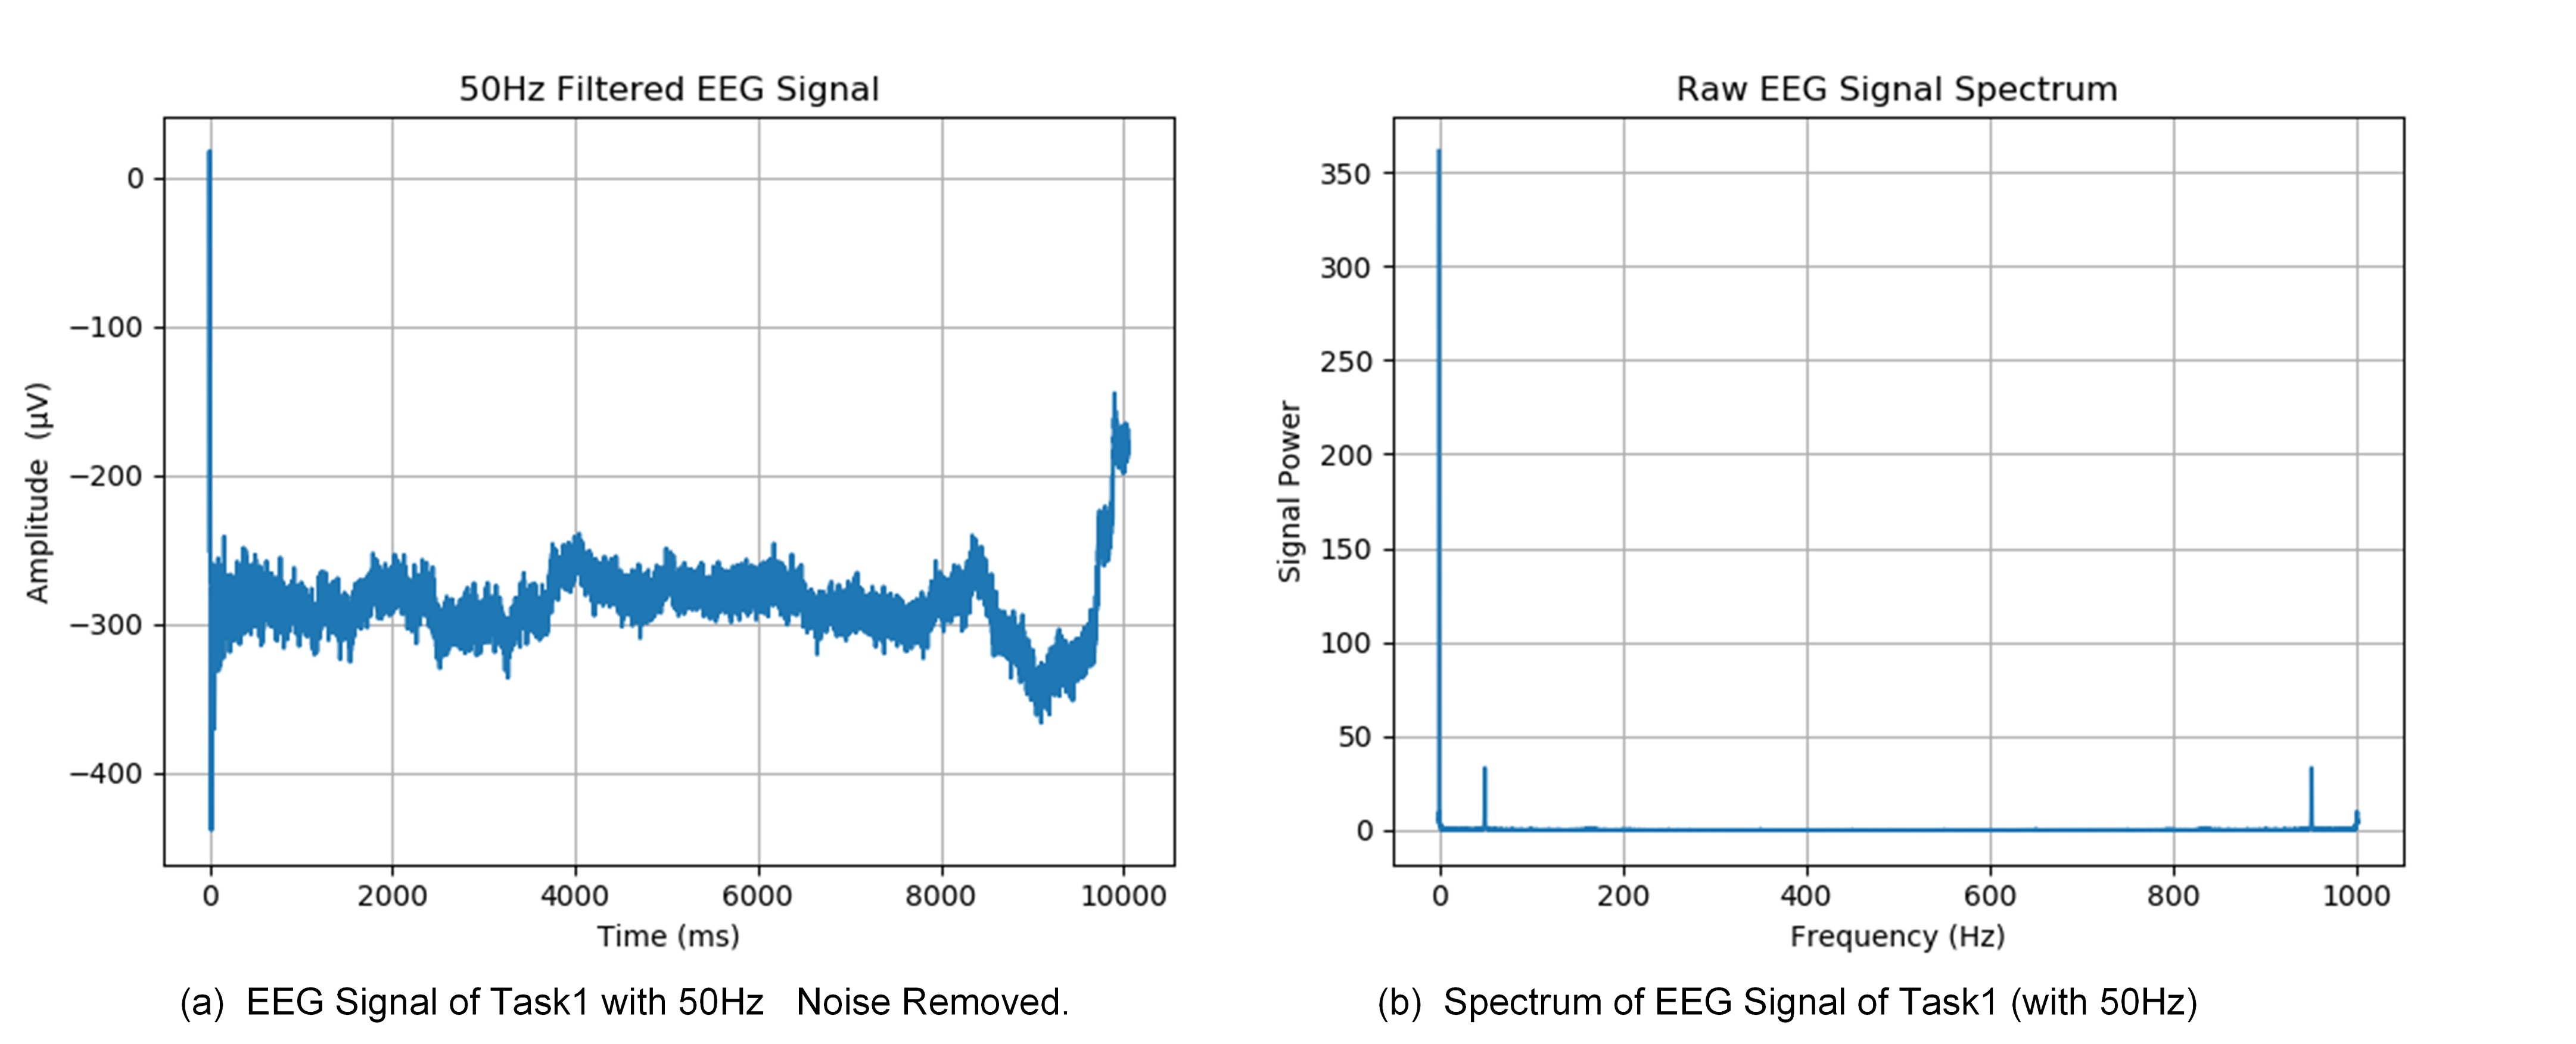
\includegraphics[width=\linewidth]{Figures/eeg_raw.jpg} 
%	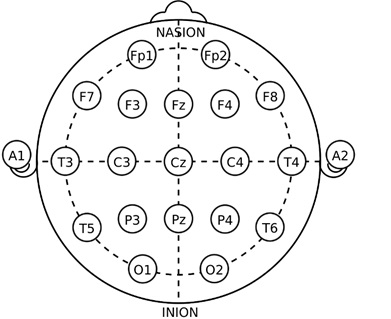
\includegraphics[width=8cm]{Figures/Brain_I20.jpg} 
	\caption{Time Domain and Spectrum of the EGG Signal for Task 1.} 
	\label{eegraw} 
\end{figure}

 
The investigation of the EEG signal was done using overlapped one second EEG signal segments. To account for the possible delays of the filters and the time required by the subject to relax, the relax sample segments were taken from the samples corresponding to 1.5 seconds after the EEG recording was initiated. The conscious signal segments were taken from four seconds up to eight seconds since the start of the recording. The analysis of the conscious signal was done on one-second overlapped segments as shown in Figure \ref{segments}.

\begin{figure}[hbt!]
	\centering
	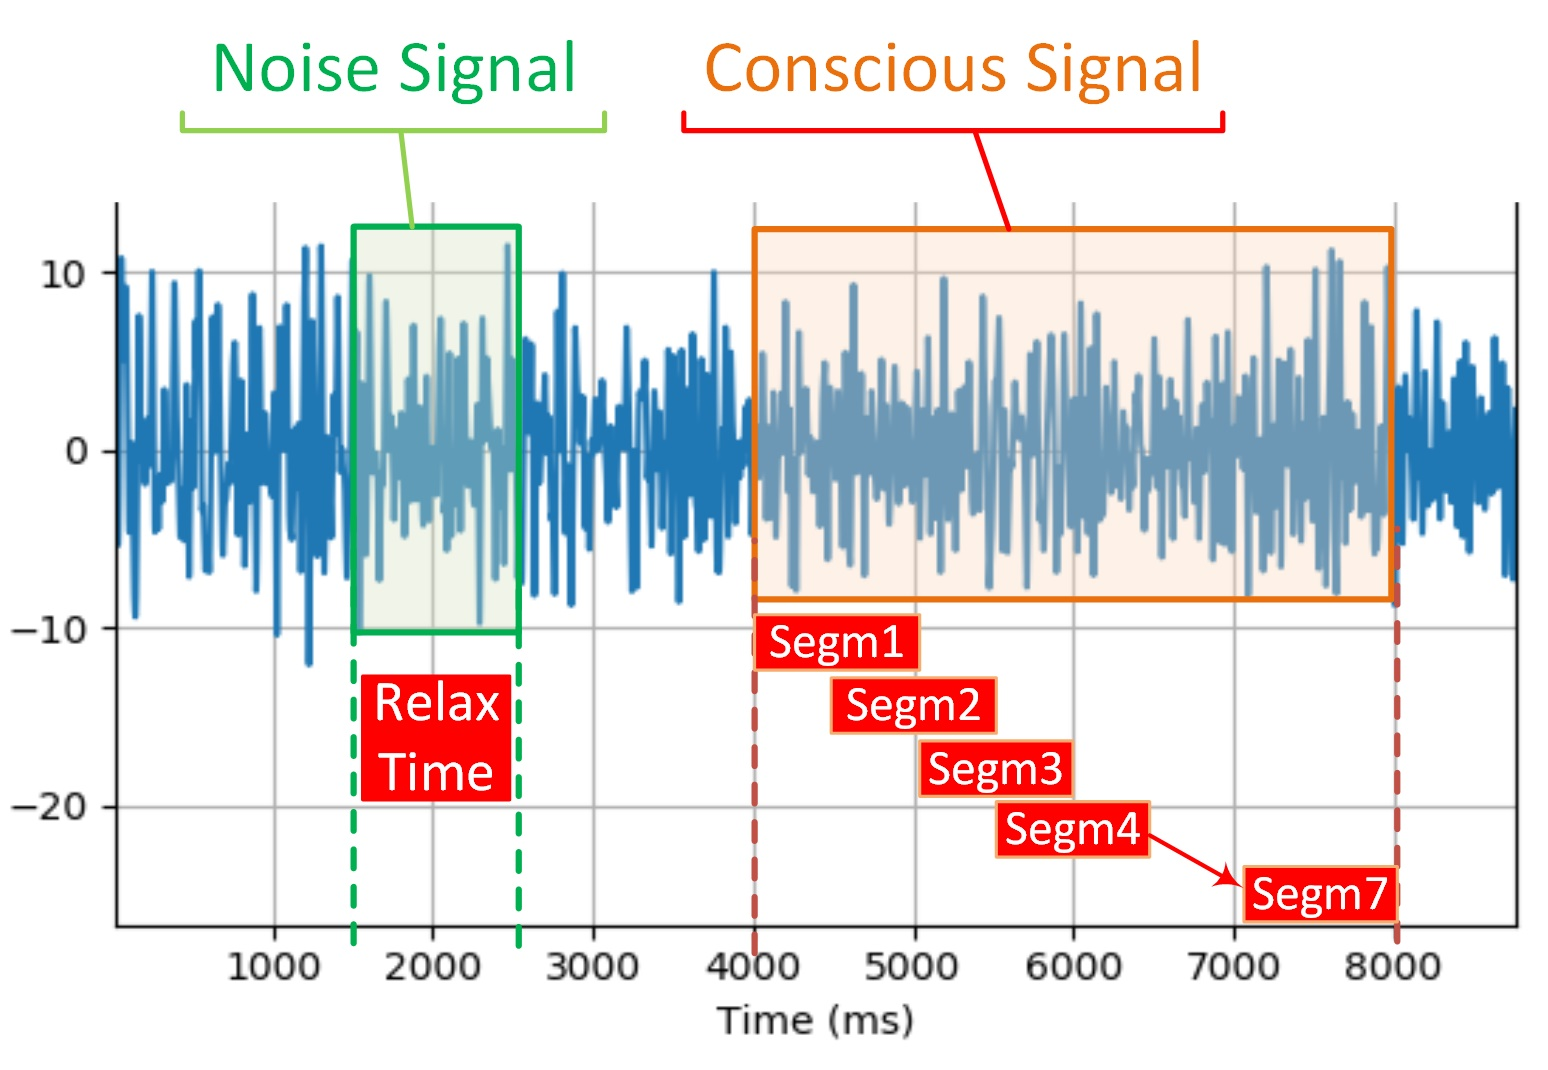
\includegraphics[width=\linewidth]{Figures/segments.jpg} 
%	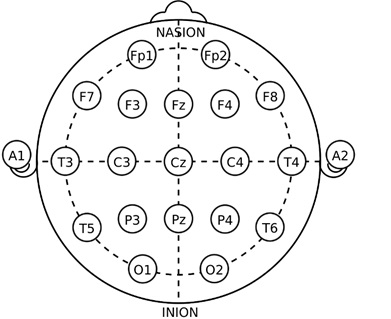
\includegraphics[width=8cm]{Figures/Brain_I20.jpg} 
	\caption{Segmentation of the EEG Signal.} 
	\label{segments} 
\end{figure}

\subsection{\bf{The 10Hz Peak Investigation:}}
The motor imagery brain activity has an effect on different frequencies in the alpha and the beta bands \citep{Pfurtscheller2000, Khulman1978}. One of the investigations of this project is related to the effect of the conscious brain activity on the 10Hz frequency. To this end the spectrum of the alpha band EEG signal obtained during the relax period is examined with respect to the spectrum of alpha band EEG signal obtained during the conscious brain activity period. Figure \ref{relaxed} shows the alpha band spectrum of the recorded signal during the relaxed period. Because imagery move activities affect other frequencies as well, the right part of Figure \ref{relaxed} also shows the frequencies up to 40Hz. 


 \begin{figure}[hbt!]
	\centering
	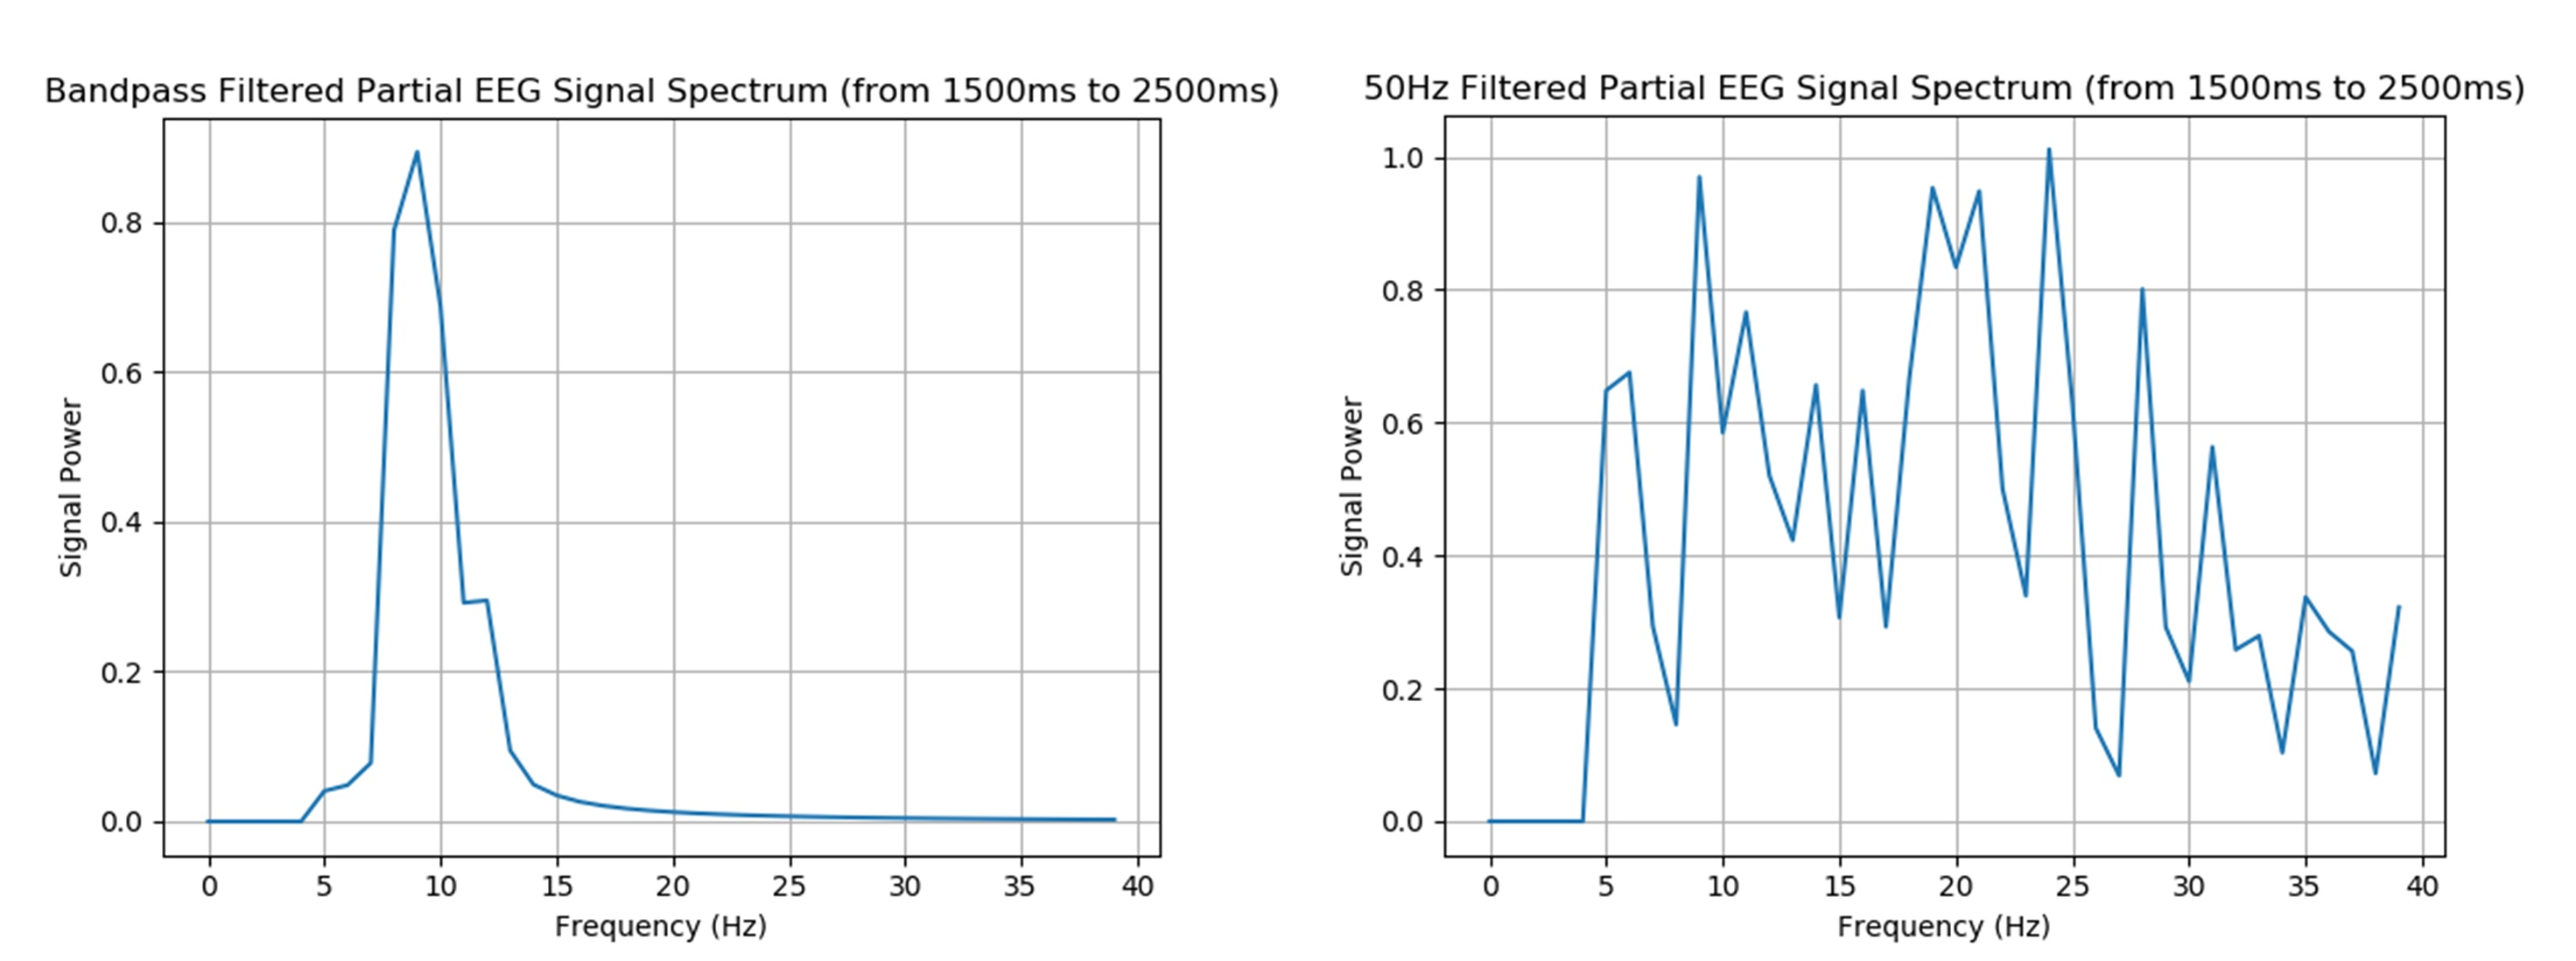
\includegraphics[width=\linewidth]{Figures/relaxed.jpg} 
%	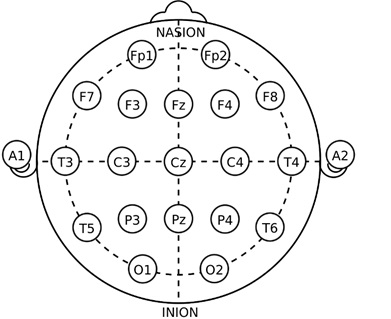
\includegraphics[width=8cm]{Figures/Brain_I20.jpg} 
	\caption{Spectrum of Subject Relax Interval (Task1).} 
	\label{relaxed} 
\end{figure}

From the filtered signal it can be seen that there is a peak at 9Hz, while from the unfiltered signal it can be seen that there are also peaks on other frequencies around 20Hz and 25 Hz. During the relaxed period, for this task, these peaks have a strength close to the strength of the 8Hz or 9Hz frequencies. The waveforms shown in Figure \ref{spectrum1} represent the spectrum during the motor imagery activity, from 4 seconds to 8 seconds. By observing the waveforms it can be seen that there are peaks at all frequencies in the alpha band. By observing the 10Hz peak in Figure  \ref{spectrum1}  are shifted to lower or higher frequencies, therefore the peaks in Figure  \ref{spectrum1}b are due to the peaks occurring at different time intervals within the four second interval. Furthermore, from the waveform of the unfiltered signal, it can be seen that the alpha band peaks are higher than those in the 18Hz to 30Hz zone.



 \begin{figure}%[hbt!]
	\centering
	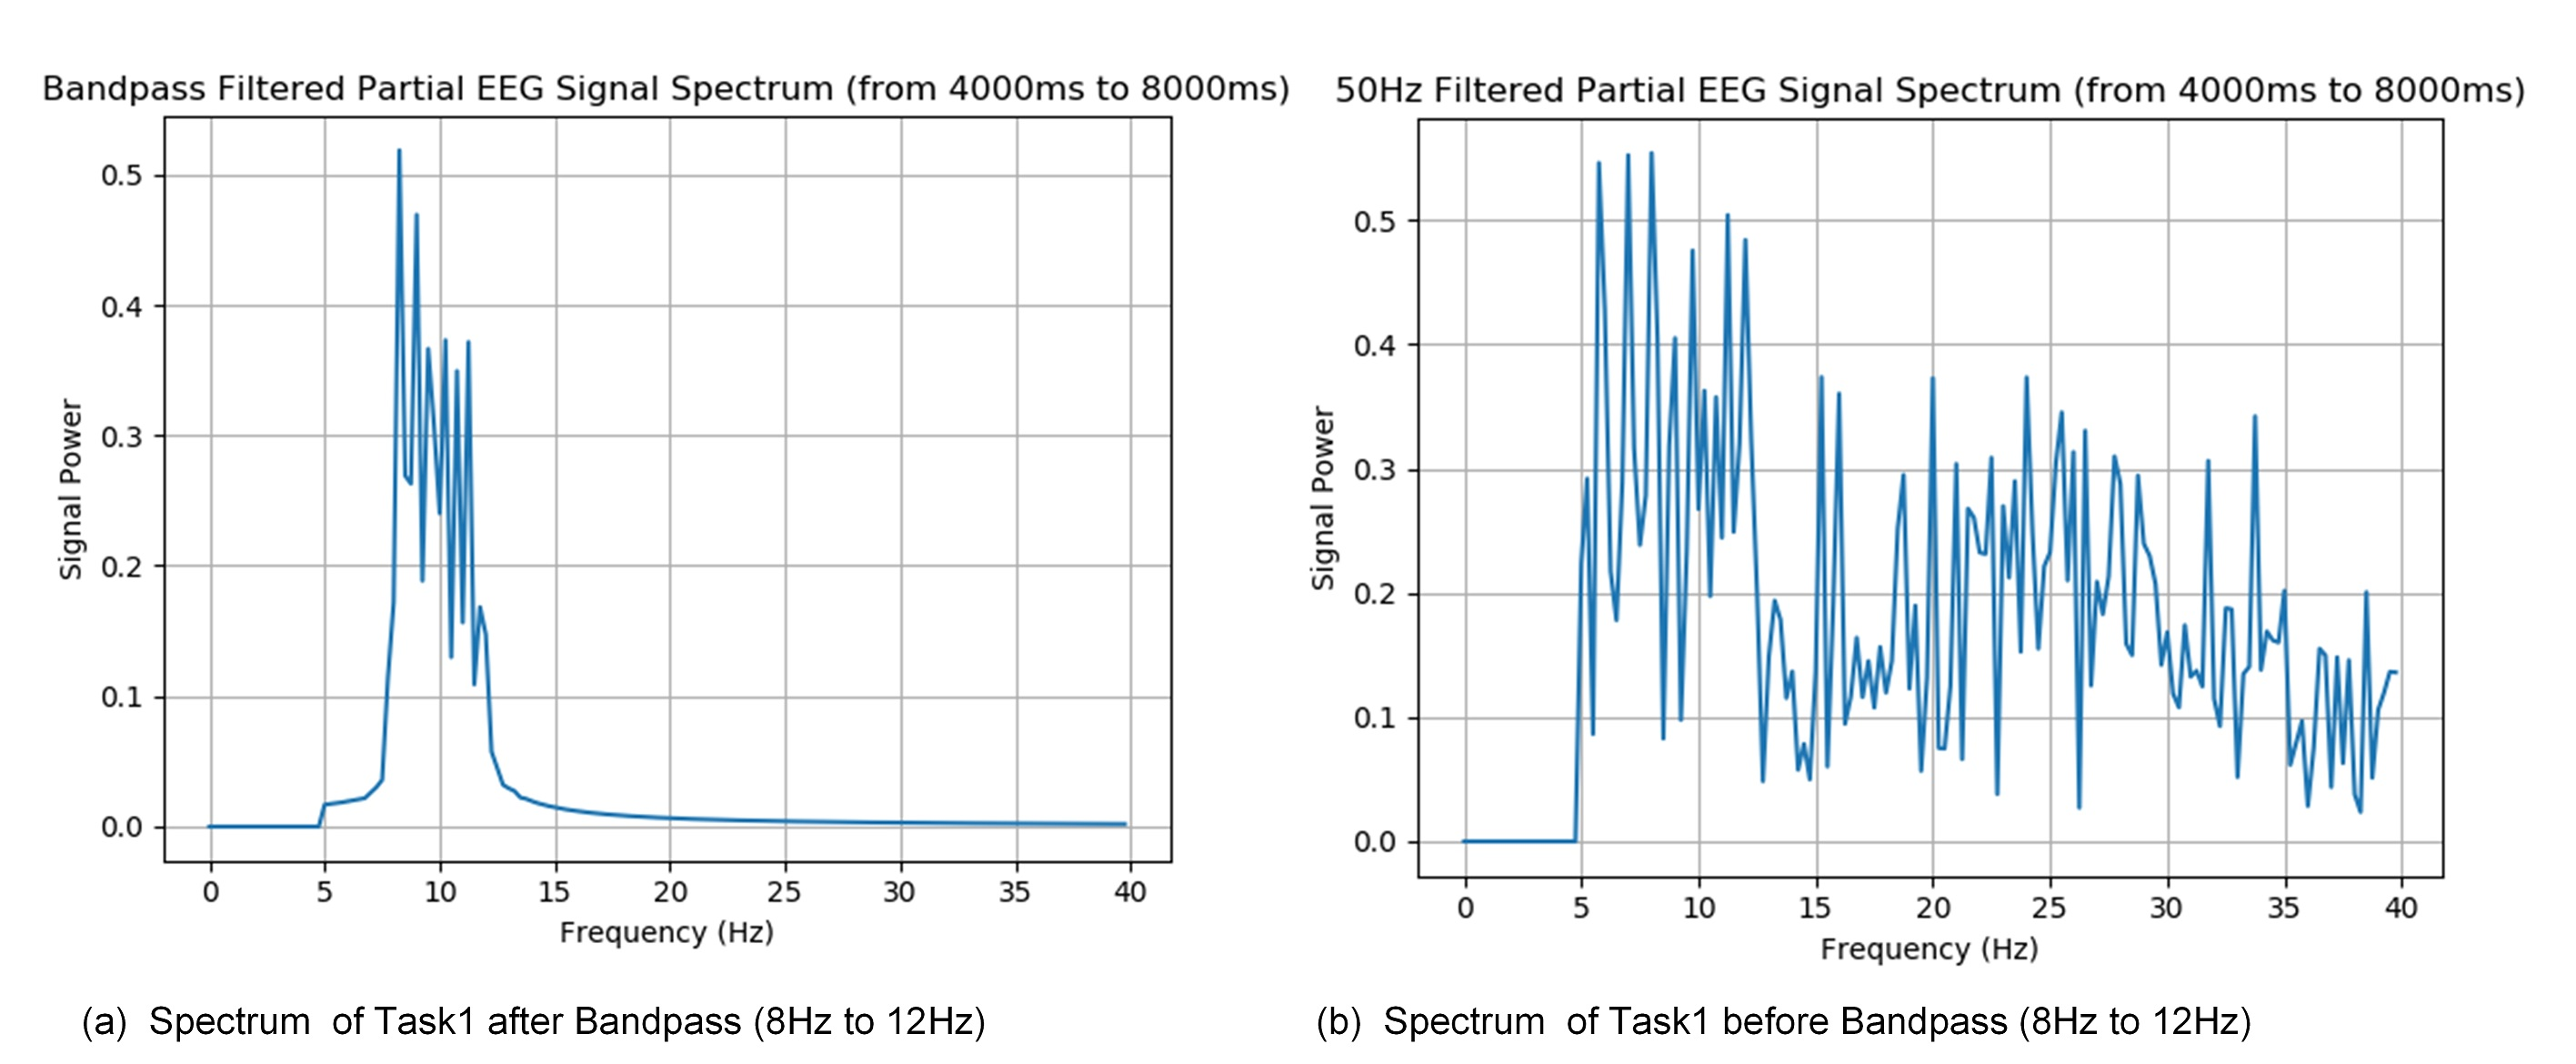
\includegraphics[width=\linewidth]{Figures/spectrum1.jpg} 
%	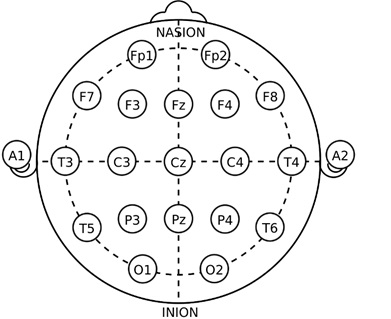
\includegraphics[width=8cm]{Figures/Brain_I20.jpg} 
	\caption{Spectrum for Task1 for the duration from 4s to 8s.} 
	\label{spectrum1} 
\end{figure}



The peaks on each one of the frequencies of the alpha zone shown in Figure \ref{spectrum1}, as well as the spectrum obtained during shorter signal segments were also examined. Figure \ref{task1_10} shows the spectrum for one-second signal segments starting at 4s, 5s, 6s, and 7s. From these spectrum diagrams it can be seen that there is also one distinguished peak around 10Hz, but this shifts either to slightly lower or higher frequencies (9Hz or 11Hz). These peak shifts are in accordance with the observations of \citep{Pfurtscheller2000, Khulman1978}.  


Similar observations can be made by examining the spectrum of the EEG signals in the alpha zone achieved with the rest of the tasks (experiments).  Figure 11 shows the spectrum for the relaxed as well the spectrum for two of the signal segments for each of the tasks 2 to 6. In all cases there always a sharp pick at around 10Hz, while in some cases a second peak is observed. Furthermore, in all experiments there is always a slight shift of the 10Hz peak either towards the 9Hz of the 11Hz frequencies. This characteristic must be taken into consideration in a BCI system looking for a signal change on the 10Hz frequency in order to make a decision on the user’s intent.

\begin{figure}%[hbt!]
	\centering
	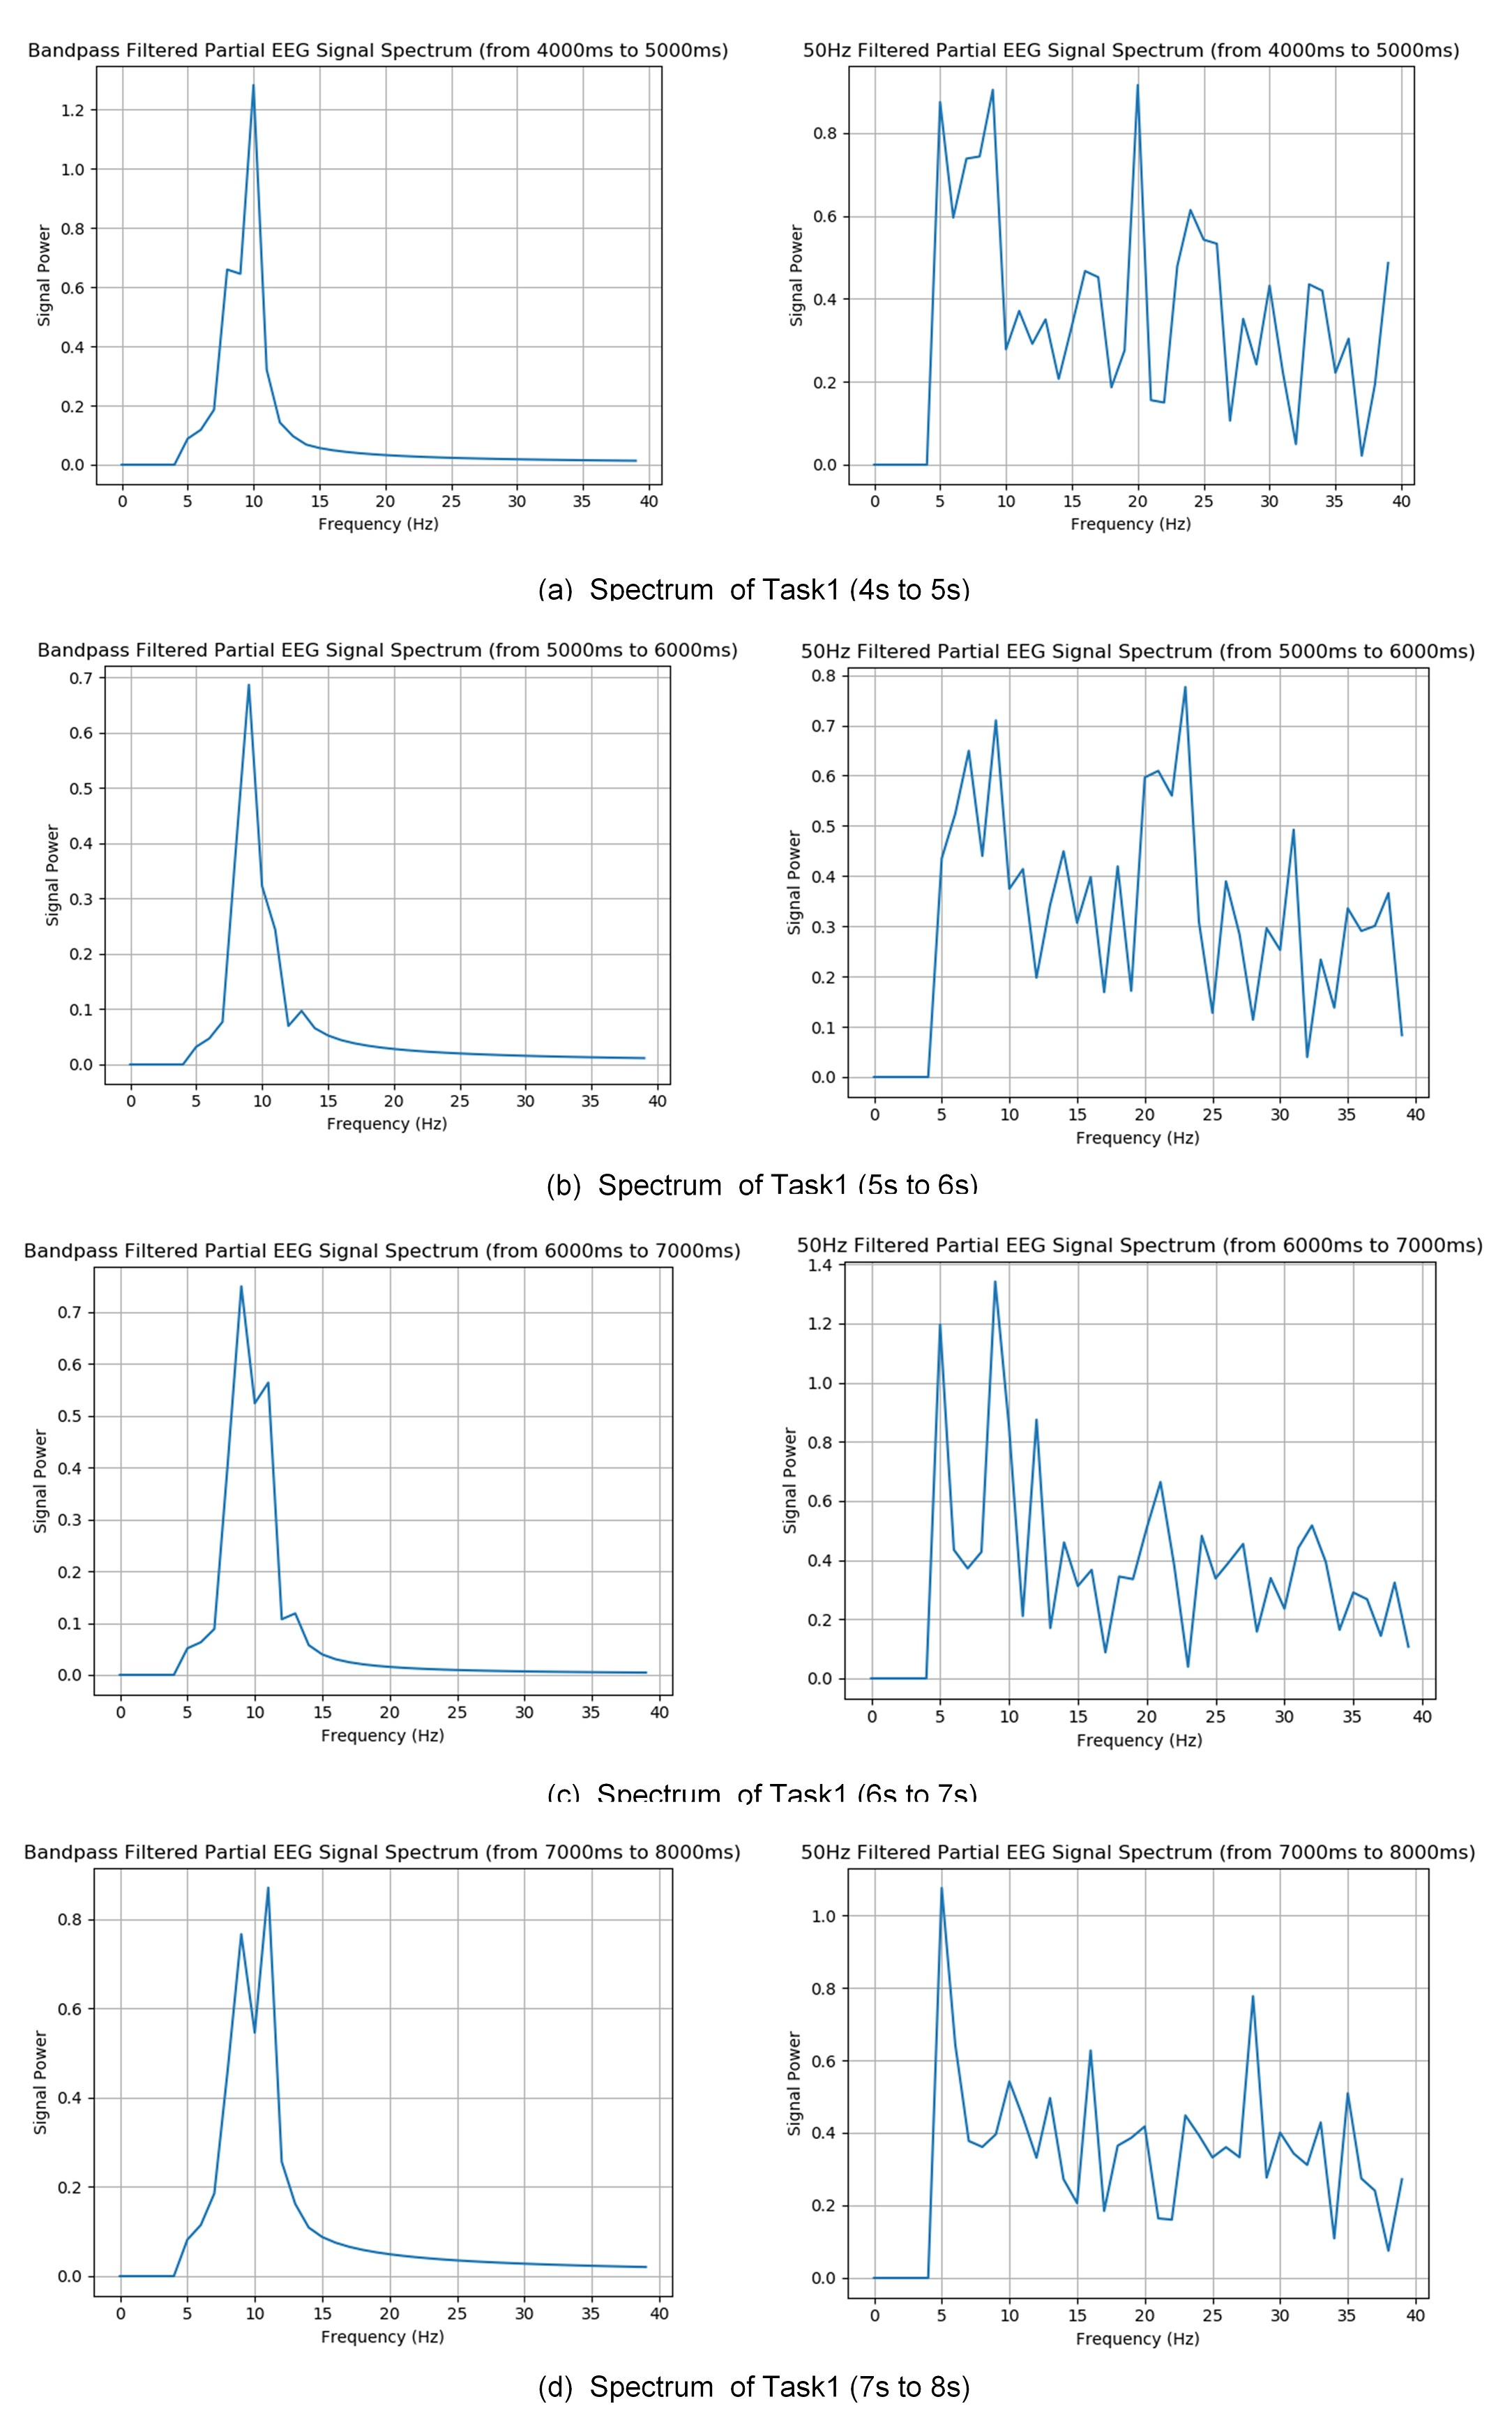
\includegraphics[width=\linewidth]{Figures/task1_10Hz.jpg} 
%	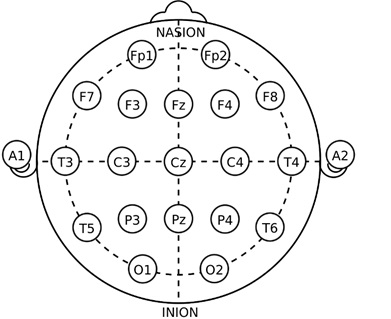
\includegraphics[width=8cm]{Figures/Brain_I20.jpg} 
	\caption{Spectrum for Task 1 (Segments of 1000ms each).} 
	\label{task1_10} 
\end{figure}


During the EEG recordings it was observed that in order to be able to use feedback, by observing the 10Hz peak, it was difficult to achieve. Even though in most cases the 10Hz band was increasing, this was not done by a significand amount. It needs practice and concentration to be able to try to perform a motor imagery operation and at the same time try to control the 10Hz frequency. It is also possible that the effect of the specific imagery move task is eventually a desynchronization event that might reduce the 10Hz instead of increasing it.  A similar case was observed when the motor imagery intent was to try and increase the 10Hz, or the 20Hz or the 30Hz frequency peaks (Figure 12). Some success was though observed when the task was to try to increase the 20Hz peak, however this is most probably the effect of the motor imagery task on the 20Hz frequency, since this is also observed in other experiments. 


\begin{figure}%[hbt!]
	\centering
	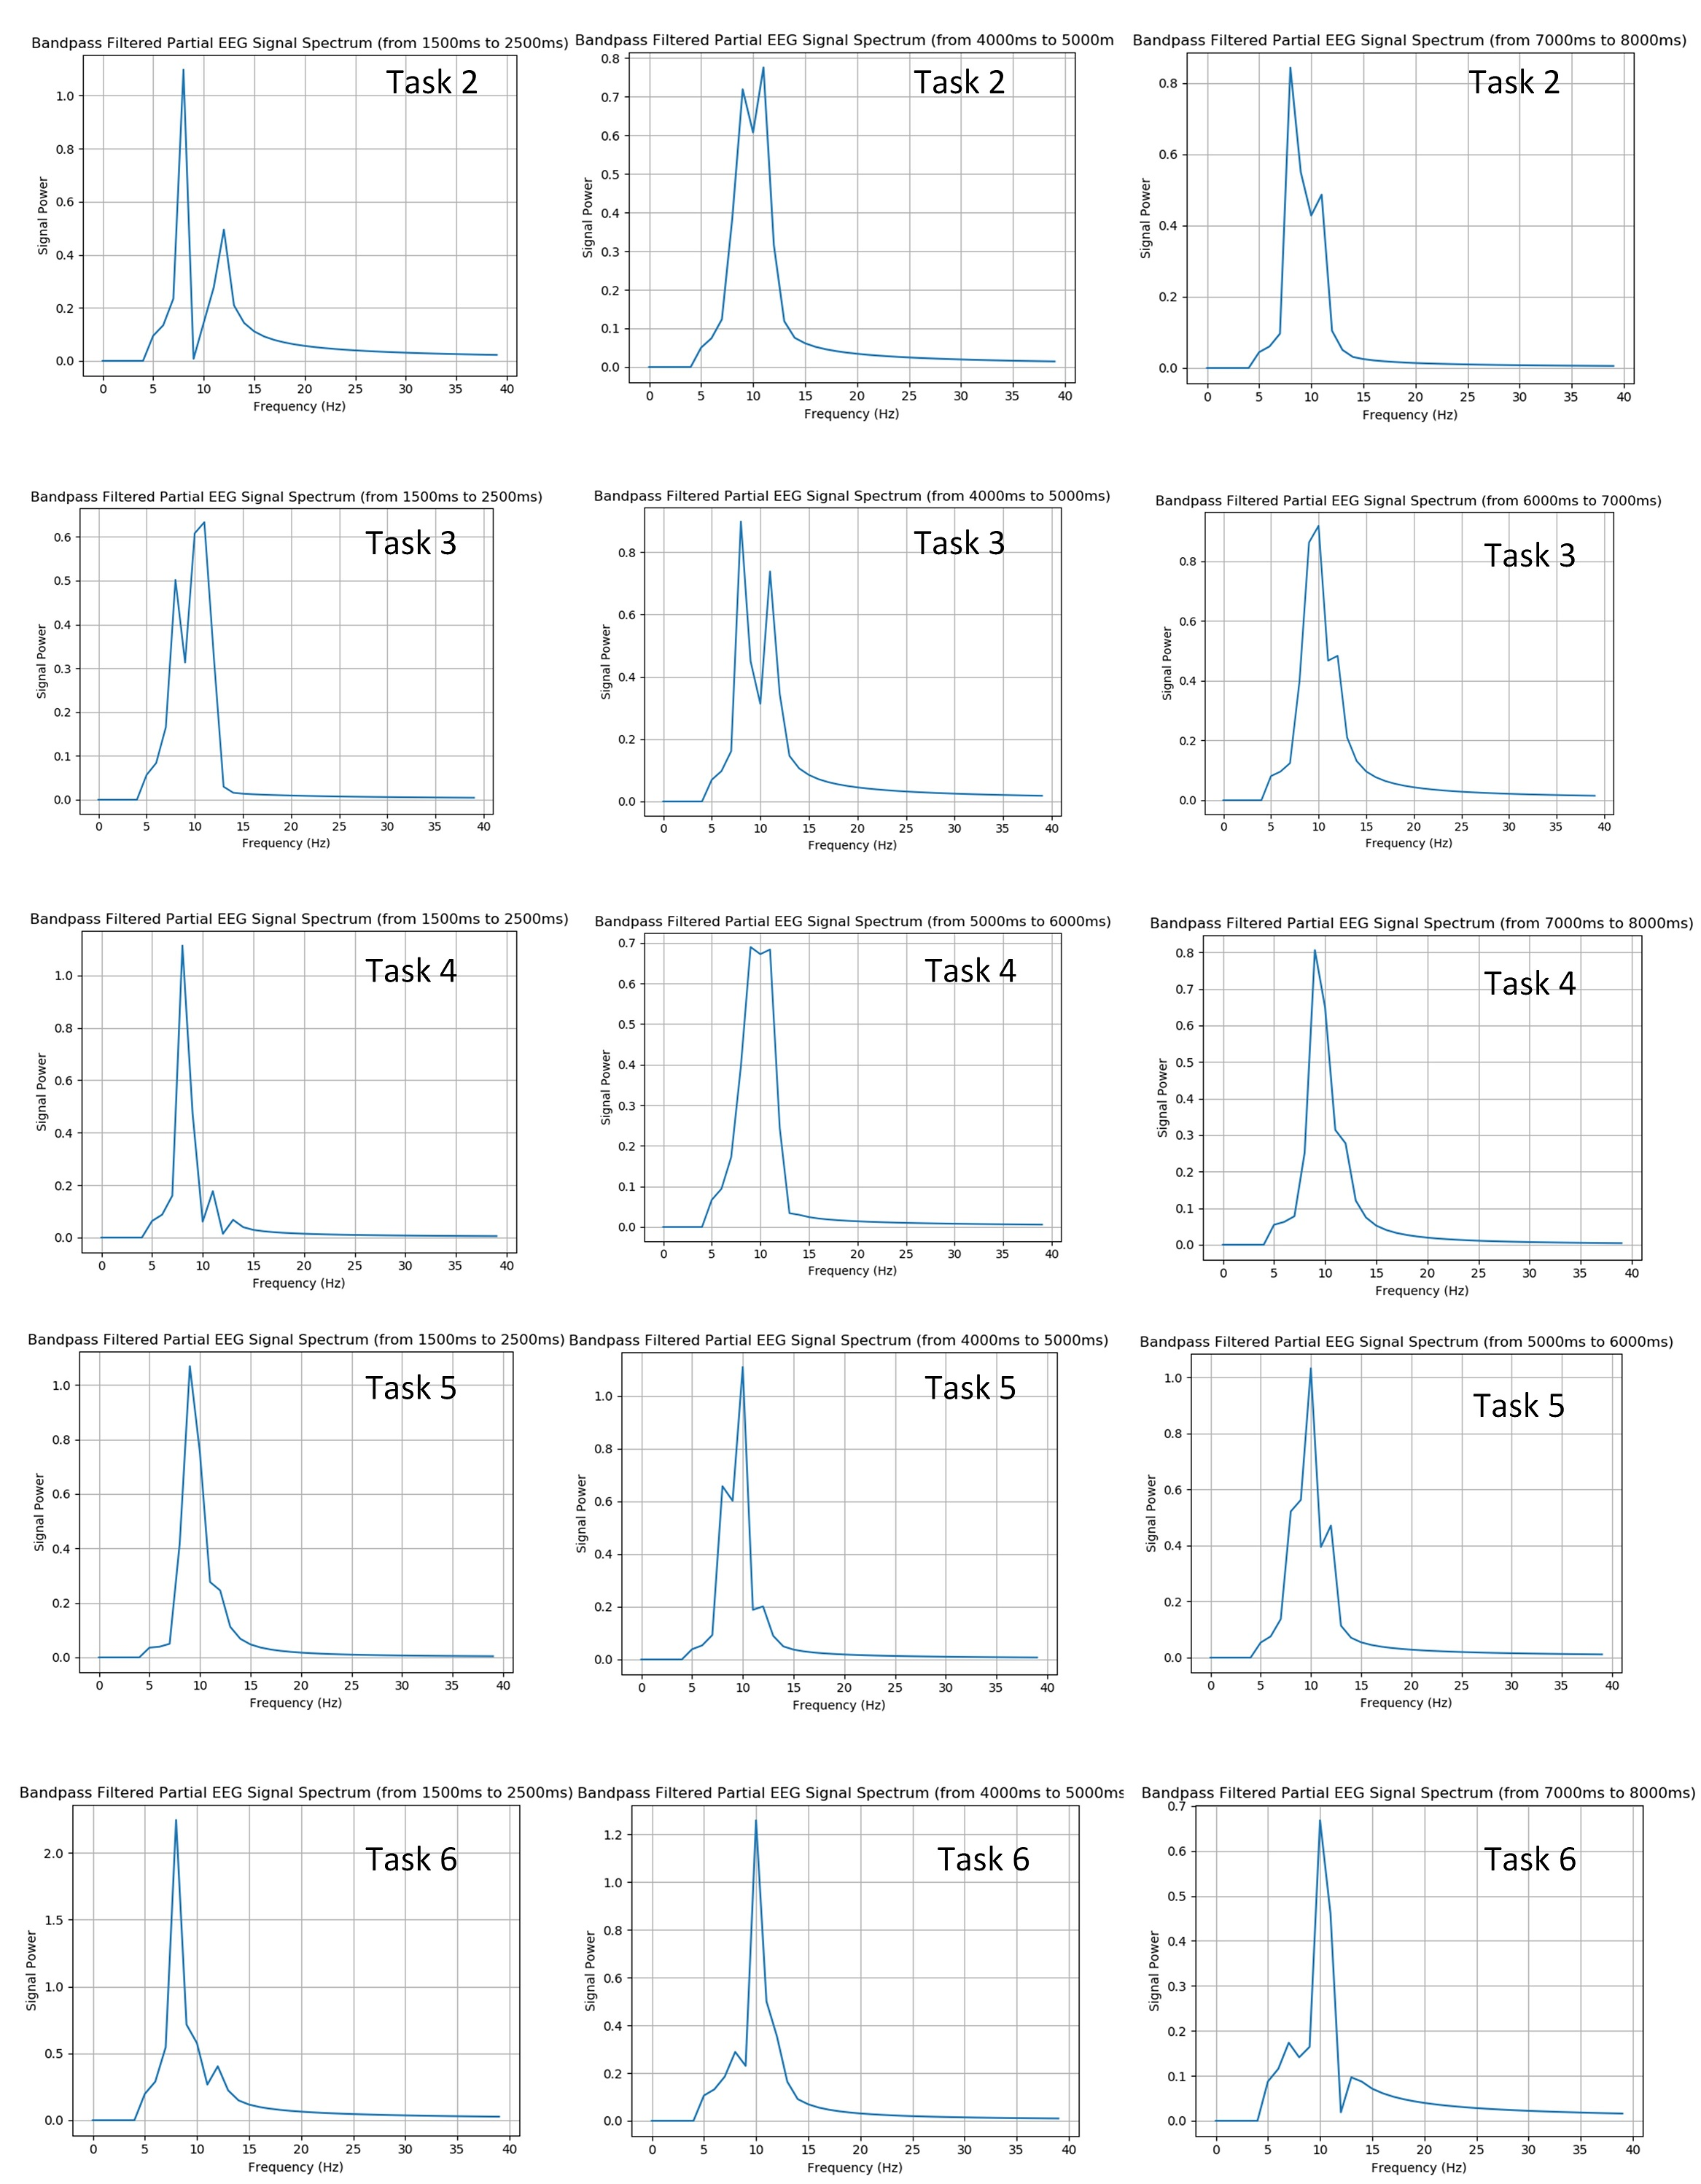
\includegraphics[width=\linewidth]{Figures/filteredAll.jpg} 
%	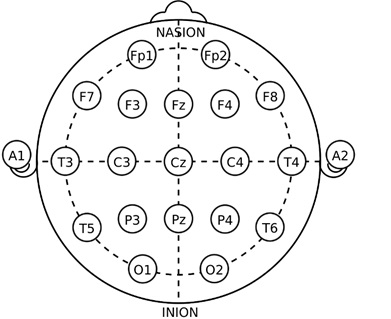
\includegraphics[width=8cm]{Figures/Brain_I20.jpg} 
	\caption{Filtered Spectrum for Task2 to Task6.} 
	\label{all_tasks_filt} 
\end{figure}

By observing the spectrum of the unfiltered signal, it can be seen that the picks in the beta frequency zone are also affected by the motor imagery process. Fluctuations are observed on the 10Hz and other 20Hz that can be used in BCI with Fp1 given that the SNR is high enough to enable the safe detection.


\begin{figure}%[hbt!]
	\centering
	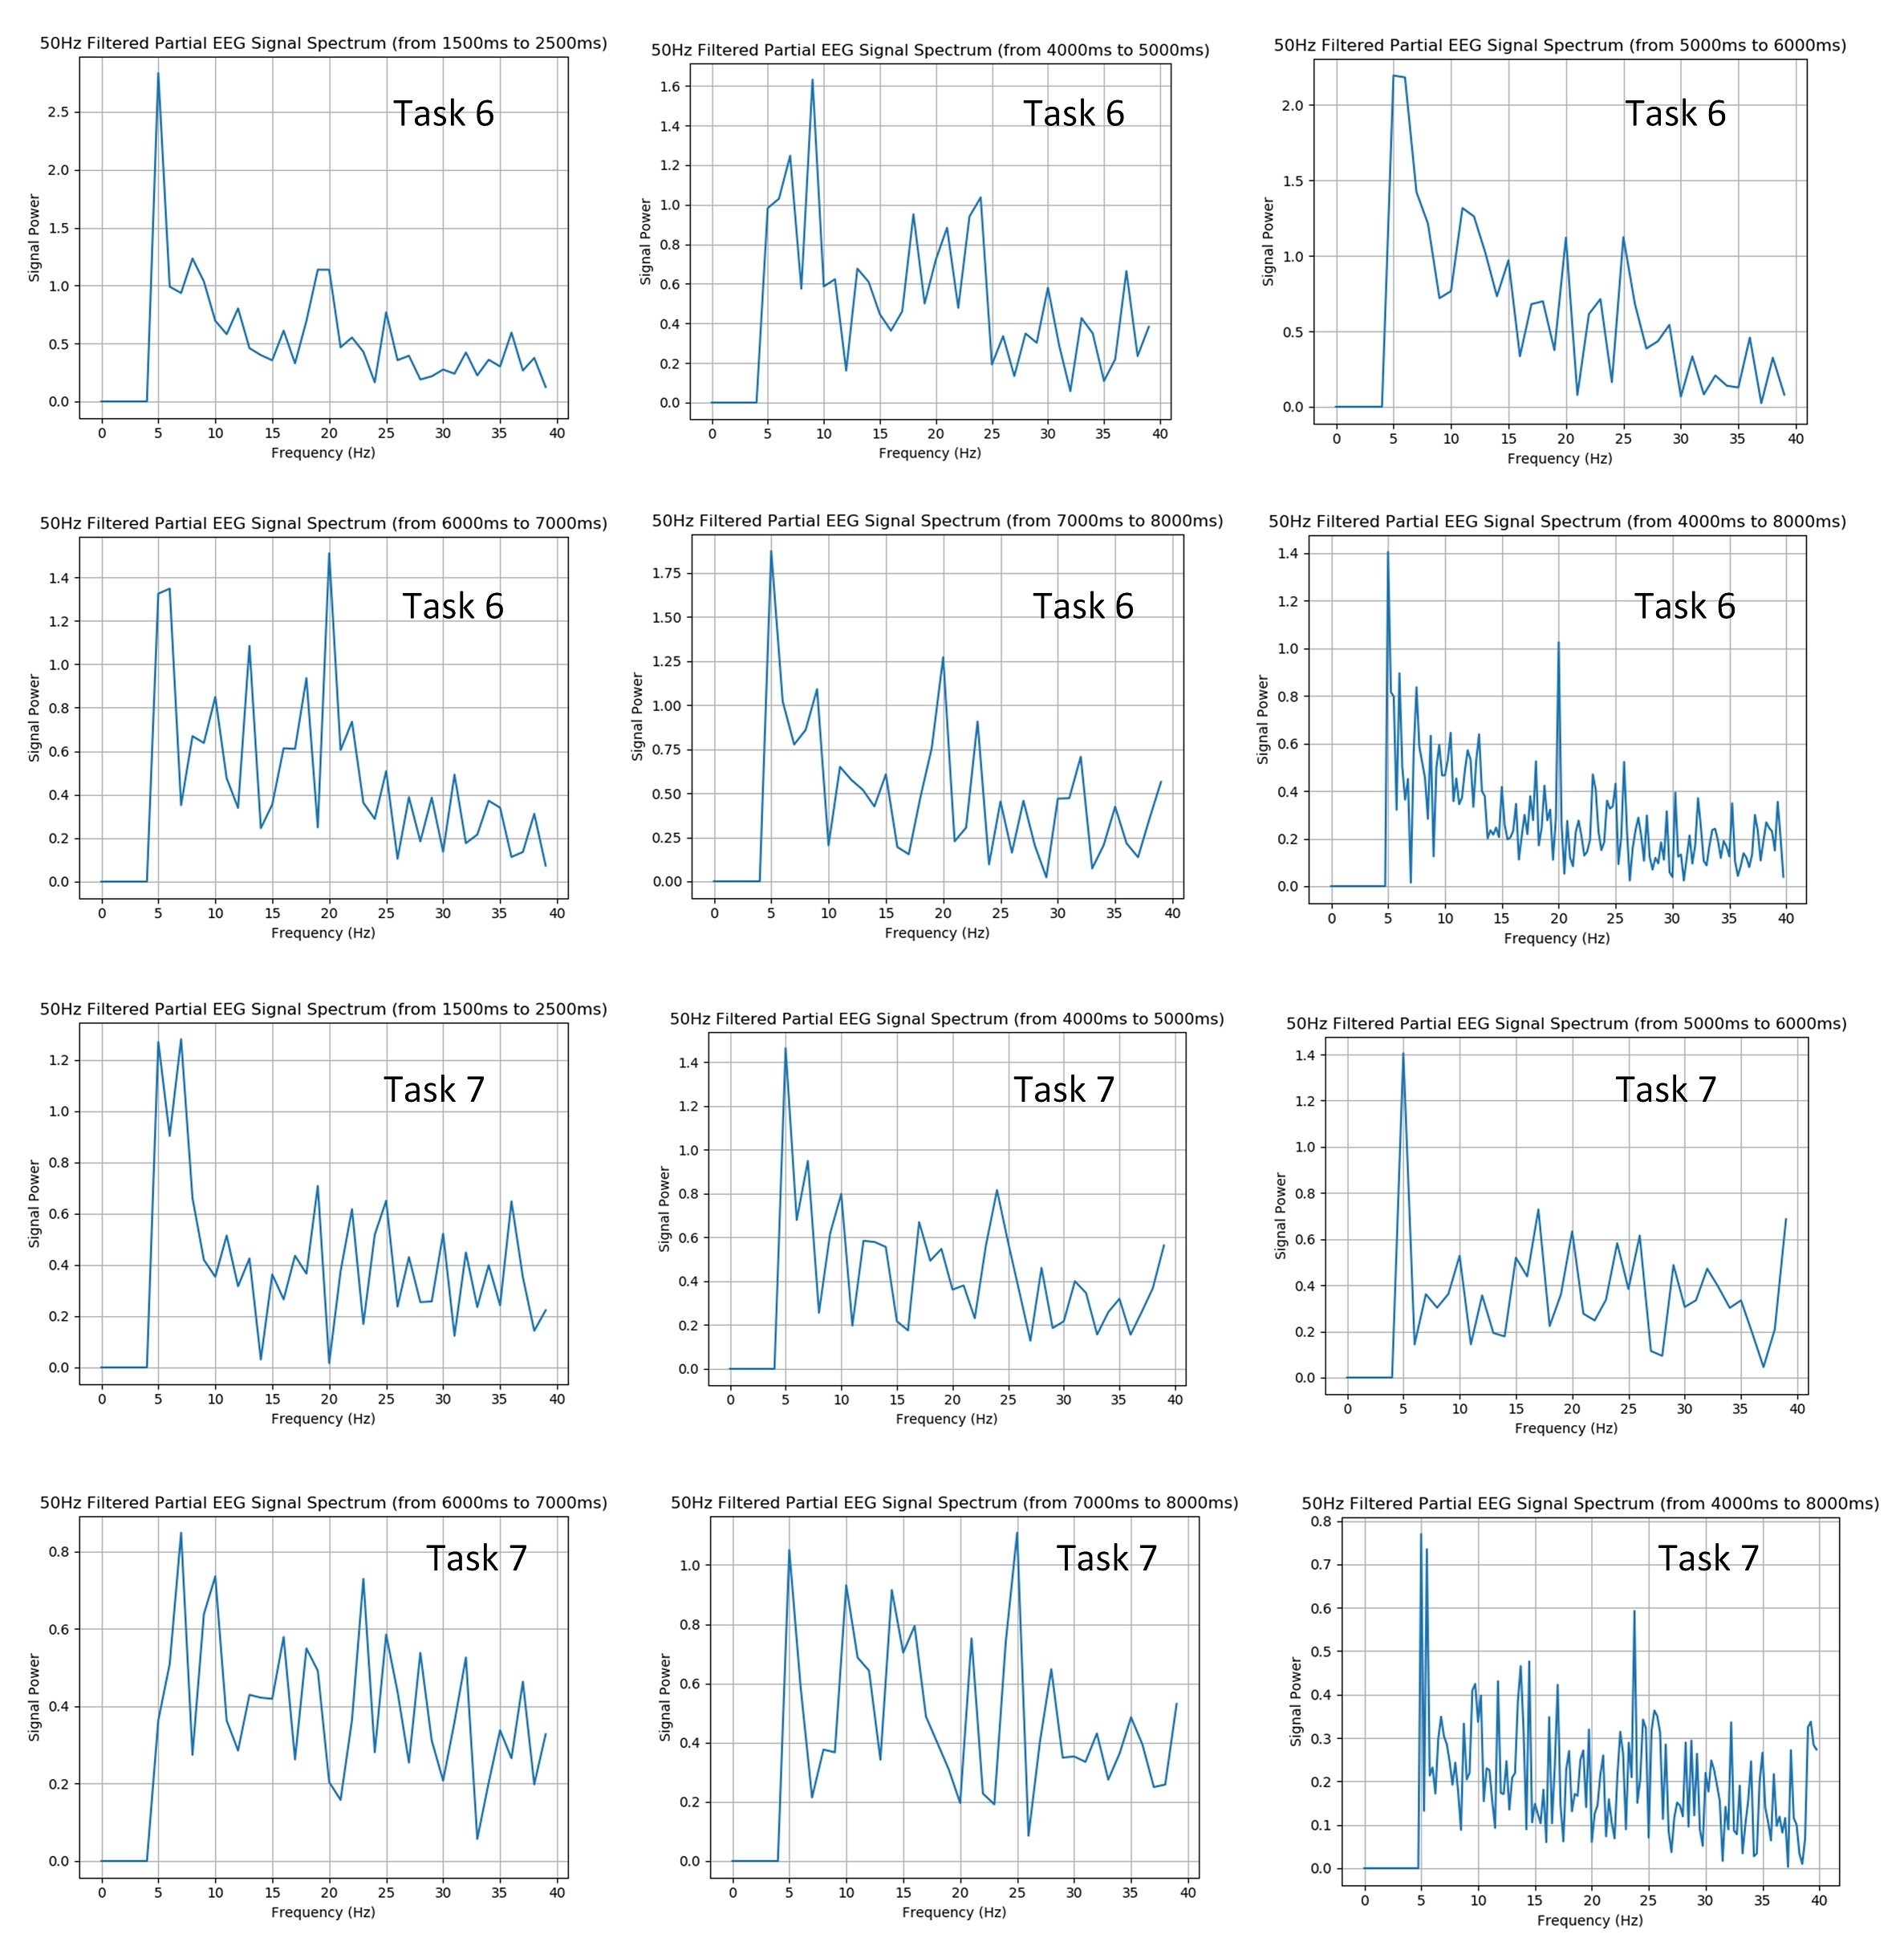
\includegraphics[width=\linewidth]{Figures/Hz102030.jpg} 
%	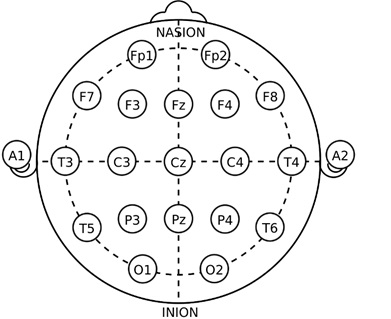
\includegraphics[width=8cm]{Figures/Brain_I20.jpg} 
	\caption{Experiments trying to increase the 20Hz and 30Hz peaks.} 
	\label{Hz2030} 
\end{figure}

\subsection{\bf{Signal-to-Noise Ratio:}}
In order to determine if EEG signals recorded from a single electrode attached on the Fp1 position can be reliable detected, it is necessary to compute the SNR of the recorded EEG signals and then compare them with the SNR Wall. If the EEG signal SNR is greater than the SNR Wall value then the BCI system with a single electrode attached on Fp1 can reliably detect an EEG signal.

The SNR for each signal segment of the recorded EEG signals was calculated using the procedure described in the “Methodology” chapter, where two approaches were described. The first one is based on the ratio of the variance of the conscious signal to the variance of the noise (equation 5). The second approach is based on the noise uncertainty (equation 8). The variances of the noise signal are shown in Table \ref{noise}.

\begin{table}[hbt!]
	\caption{Noise Variance}
	\label{noise}
	\centering
	\begin{tabular}{|c|c|c|l|}
	\hline
		Task &Noise Variancee & Noise Variance Ratio & Effect on SNR calculation\\
		 \hline\hline
		Task1 & 2.07E-08 & 2.05 &	SNR using Eq5 is about 3dB greater than  with Eq.8\\
		Task2 & 4.94E-09 & 0.49 &	SNR using Eq5 is about 3dB less than  with Eq.8\\
		Task3 & 9.56E-09 & 0.95 &	SNR using Eq5 is about the same as that with Eq.8\\
		Task4 & 5.09E-09 & 0.50 &	SNR using Eq5 is about 3dB less than  with Eq.8\\
		Task5 & 9.49E-09 & 0.94 &	SNR using Eq5 is about the same as that with Eq.8\\
		Task6 & 1.52E-08 & 1.50 &	SNR using Eq5 is about 1.75dB greater than  with Eq.8\\
		Task7 & 9.49E-09 & 0.94 &	SNR using Eq5 is about the same as that with Eq.8\\
		 \hline
	\end{tabular}
\end{table}


The maximum noise variance is the noise variance for Task1, while the minimum is the variance of Task2. The noise uncertainty (\textrho) is equal to 2.05 as computed with equation 6, while the overall noise variance is 1.01E-08 (computed with equation 7). Therefore, to compute the SNR using equation 5, the noise variance to be used is the one shown in table 2. To compute the SNR using equation 8, the noise variance to be used is for all tasks 1.01E-08. This will result in a change in the SNR given in table \ref{noise}. This can be verified by the plots of the SNR for all signal segments for the case of Task1 and Task3. From in Figure \ref{SNRdiff}, it can be seen that for the case of Task 1 there is a difference of about 3dB between the SNR computed with eq. 5. (series2) and the SNR computed with eq. 8. In the case of Task 3 the SNR is almost the same between the two methods. 


\begin{figure}%[hbt!]
	\centering
%	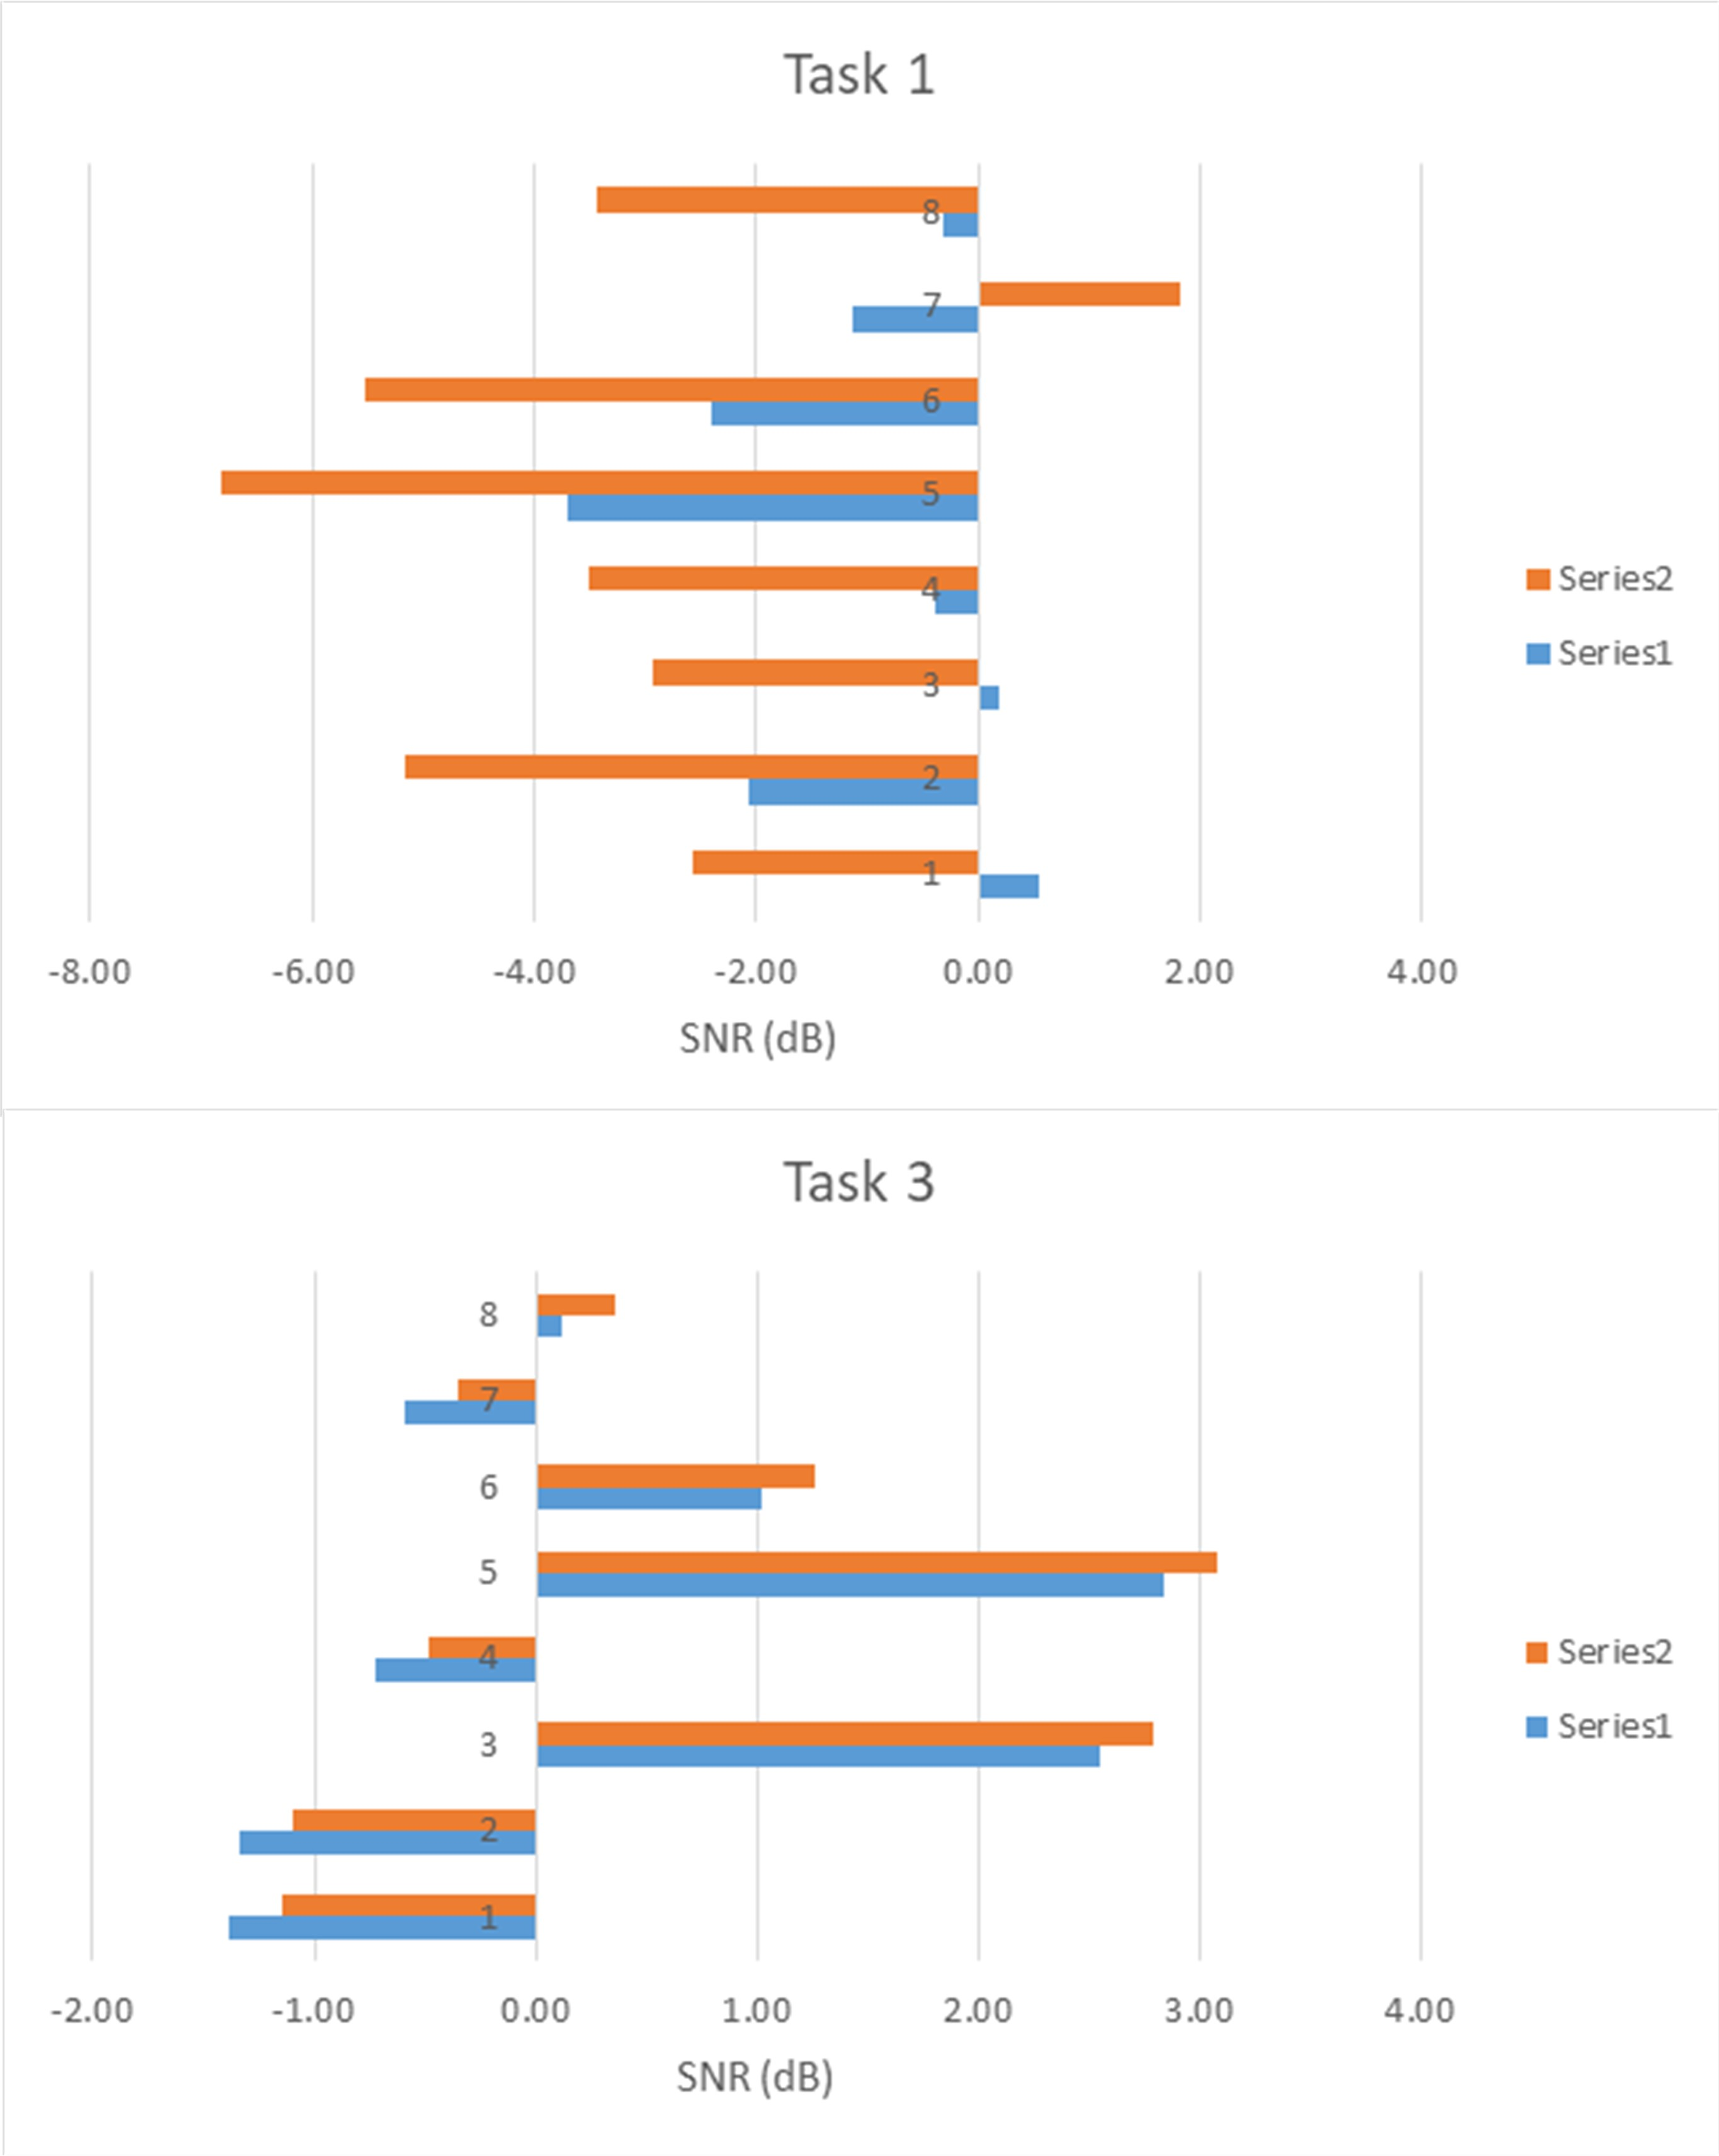
\includegraphics[width=\linewidth]{Figures/SNRchange.jpg} 
	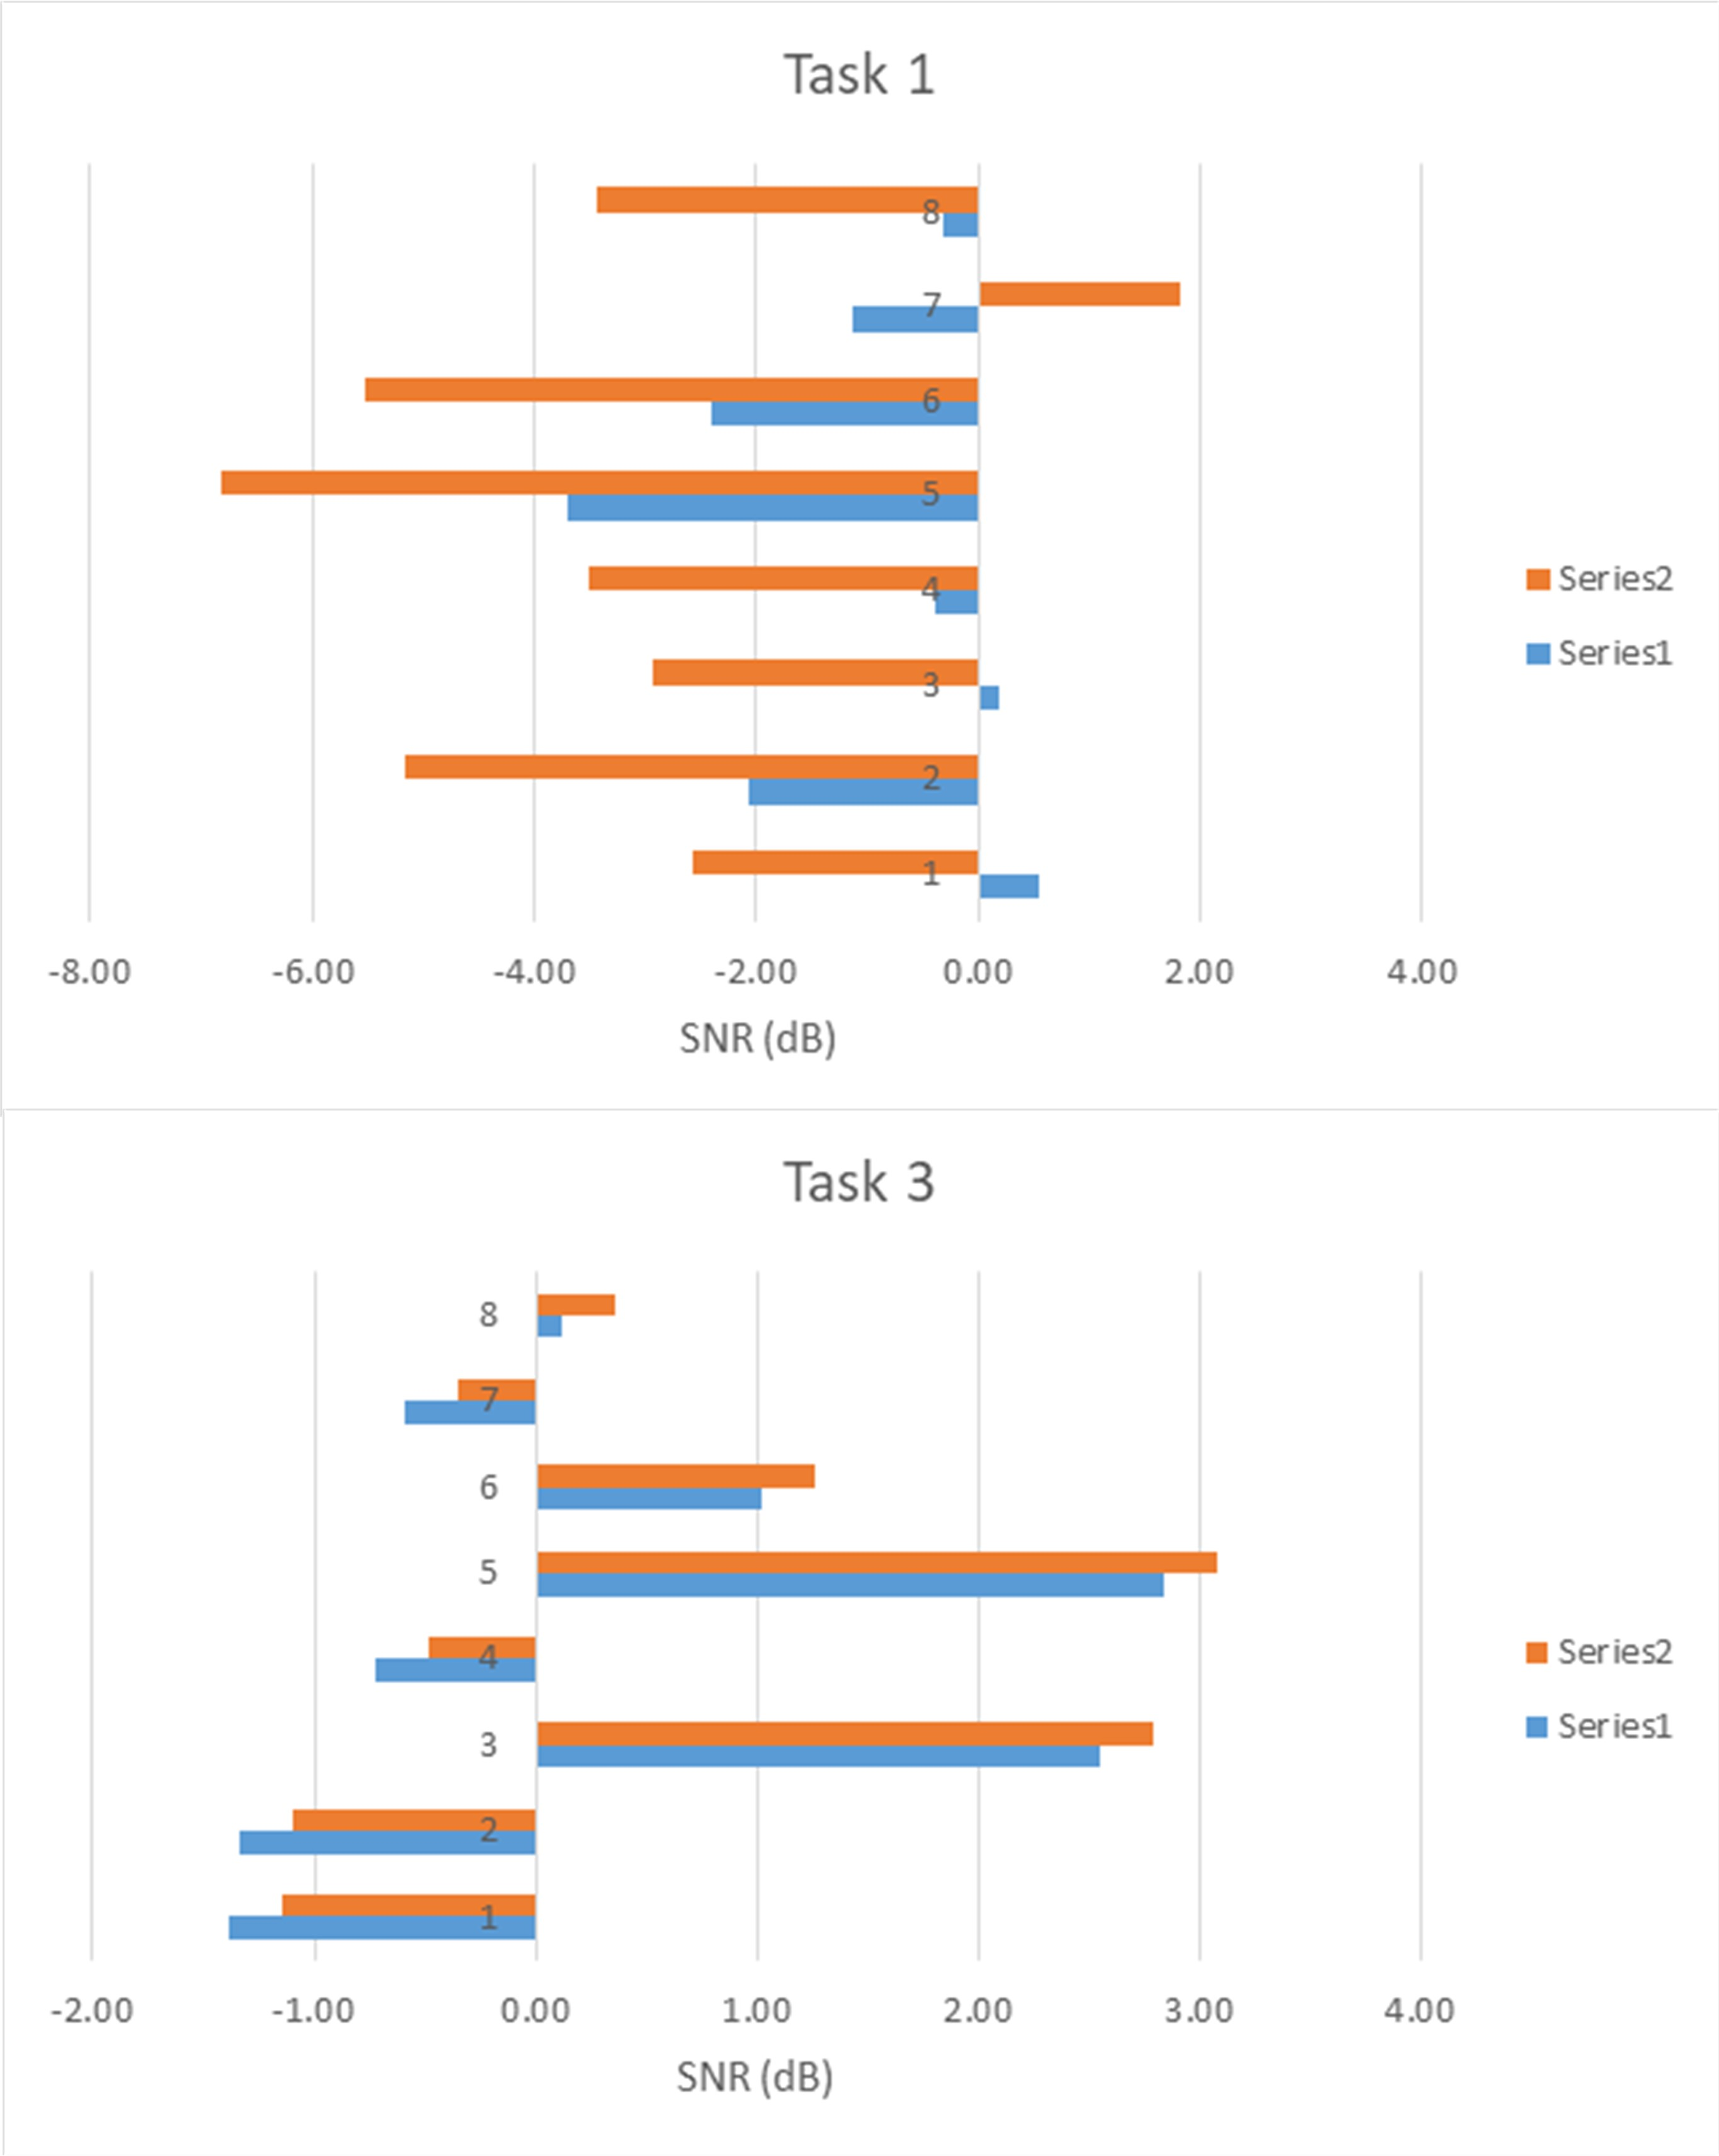
\includegraphics[width=9cm]{Figures/SNRchange.jpg} 
	\caption{SNR Difference when using Eq. 5 and Eq. 8.} 
	\label{SNRdiff} 
\end{figure}

The SNR was calculated for each signal segment. The calculated SNR values are given in Table \ref{SNRall}. Signal segments 1 to 7 correspond to the signal segments recorded during the time intervals 4s to 5s, 4.5s to 5.5s, 5s to 6s, 5.5s to 6.5s etc. The last column (column 8) corresponds to the segment for 4s to 8s.


\begin{table}[hbt!]
	\caption{ SNR for all Experiments}
	\label{SNRall}
	\centering
	\begin{tabular}{|c|c|c|c|c|c|c|c|c|}
	\hline
		%Signal Segment
		%hline
		Task & Segm. 1 & Segm. 2 & Segm. 3 & Segm. 4 & Segm. 5 & Segm. 6 & Segm. 7 & Segm. 8\\
		 \hline\hline
		%\vspace {3pt}
		Task1 &0.55 & -2.06	 &0.19 & -0.39  & 3.71 & -2.41 & -1.14 & -0.32\\
		%\vspace{3pt}
		\hline
		Task2 &1.02 & -0.61	 & -1.00 &	-1.15 & -5.01 & 	-0.64 & -1.97 & 	-0.34\\
		\hline
		Task3 & -1.38 &	 -1.34 & 2.55 & -0.72 & 2.84 & 1.02 & -0.59 & 0.11\\
		\hline
		Task4 & -3.01 &	 1.27	 & -1.08 & 0.28 & -3.05 & -3.44 & -1.82 & -0.35\\
		\hline
		Task5 & -0.71 &	 -1.00 & -2.21 & 0.10 & -0.35 & -1.73 & 0.69 & -0.88\\
		\hline
		Task6 & 3.38 &	-1.03	 & -0.97 & 0.86 & -0.35 & -0.51 & 0.69 & 0.96\\
		\hline
		Task7 &-0.71 &	-1.00 & -2.21 &	0.10 & -0.35 & -1.73 & 0.69 & -0.88\\
		 \hline
	\end{tabular}
\end{table}


The SNR for each experiment plots are shown separately in Figures \ref{SNR1} to \ref{SNR7} . These are computed using Eq. 8. On each one of these plots the values for the SNR walls are taken from (Porr B. , 2018), for three of the scenarios used (relaxed, eye blinking and solving Sudoku). The values used are the ones determined with the filter parameters EEG 8Hz to 18Hz, band pass 4Hz to 35Hz and noise reduction 1. The reason for choosing these SNR wall cases is because when using a BCI system the user will operate in a fashion similar to the Sudoku solving process. When using a BCI system, a common source of artefacts is due to eye blinking, because in most cases this is done unintentionally. The relaxed SNR wall is included as a reference because the SNR is computed using the relaxed EEG signals as the noise reference. 

\begin{figure}[hbt!]
	\centering
%	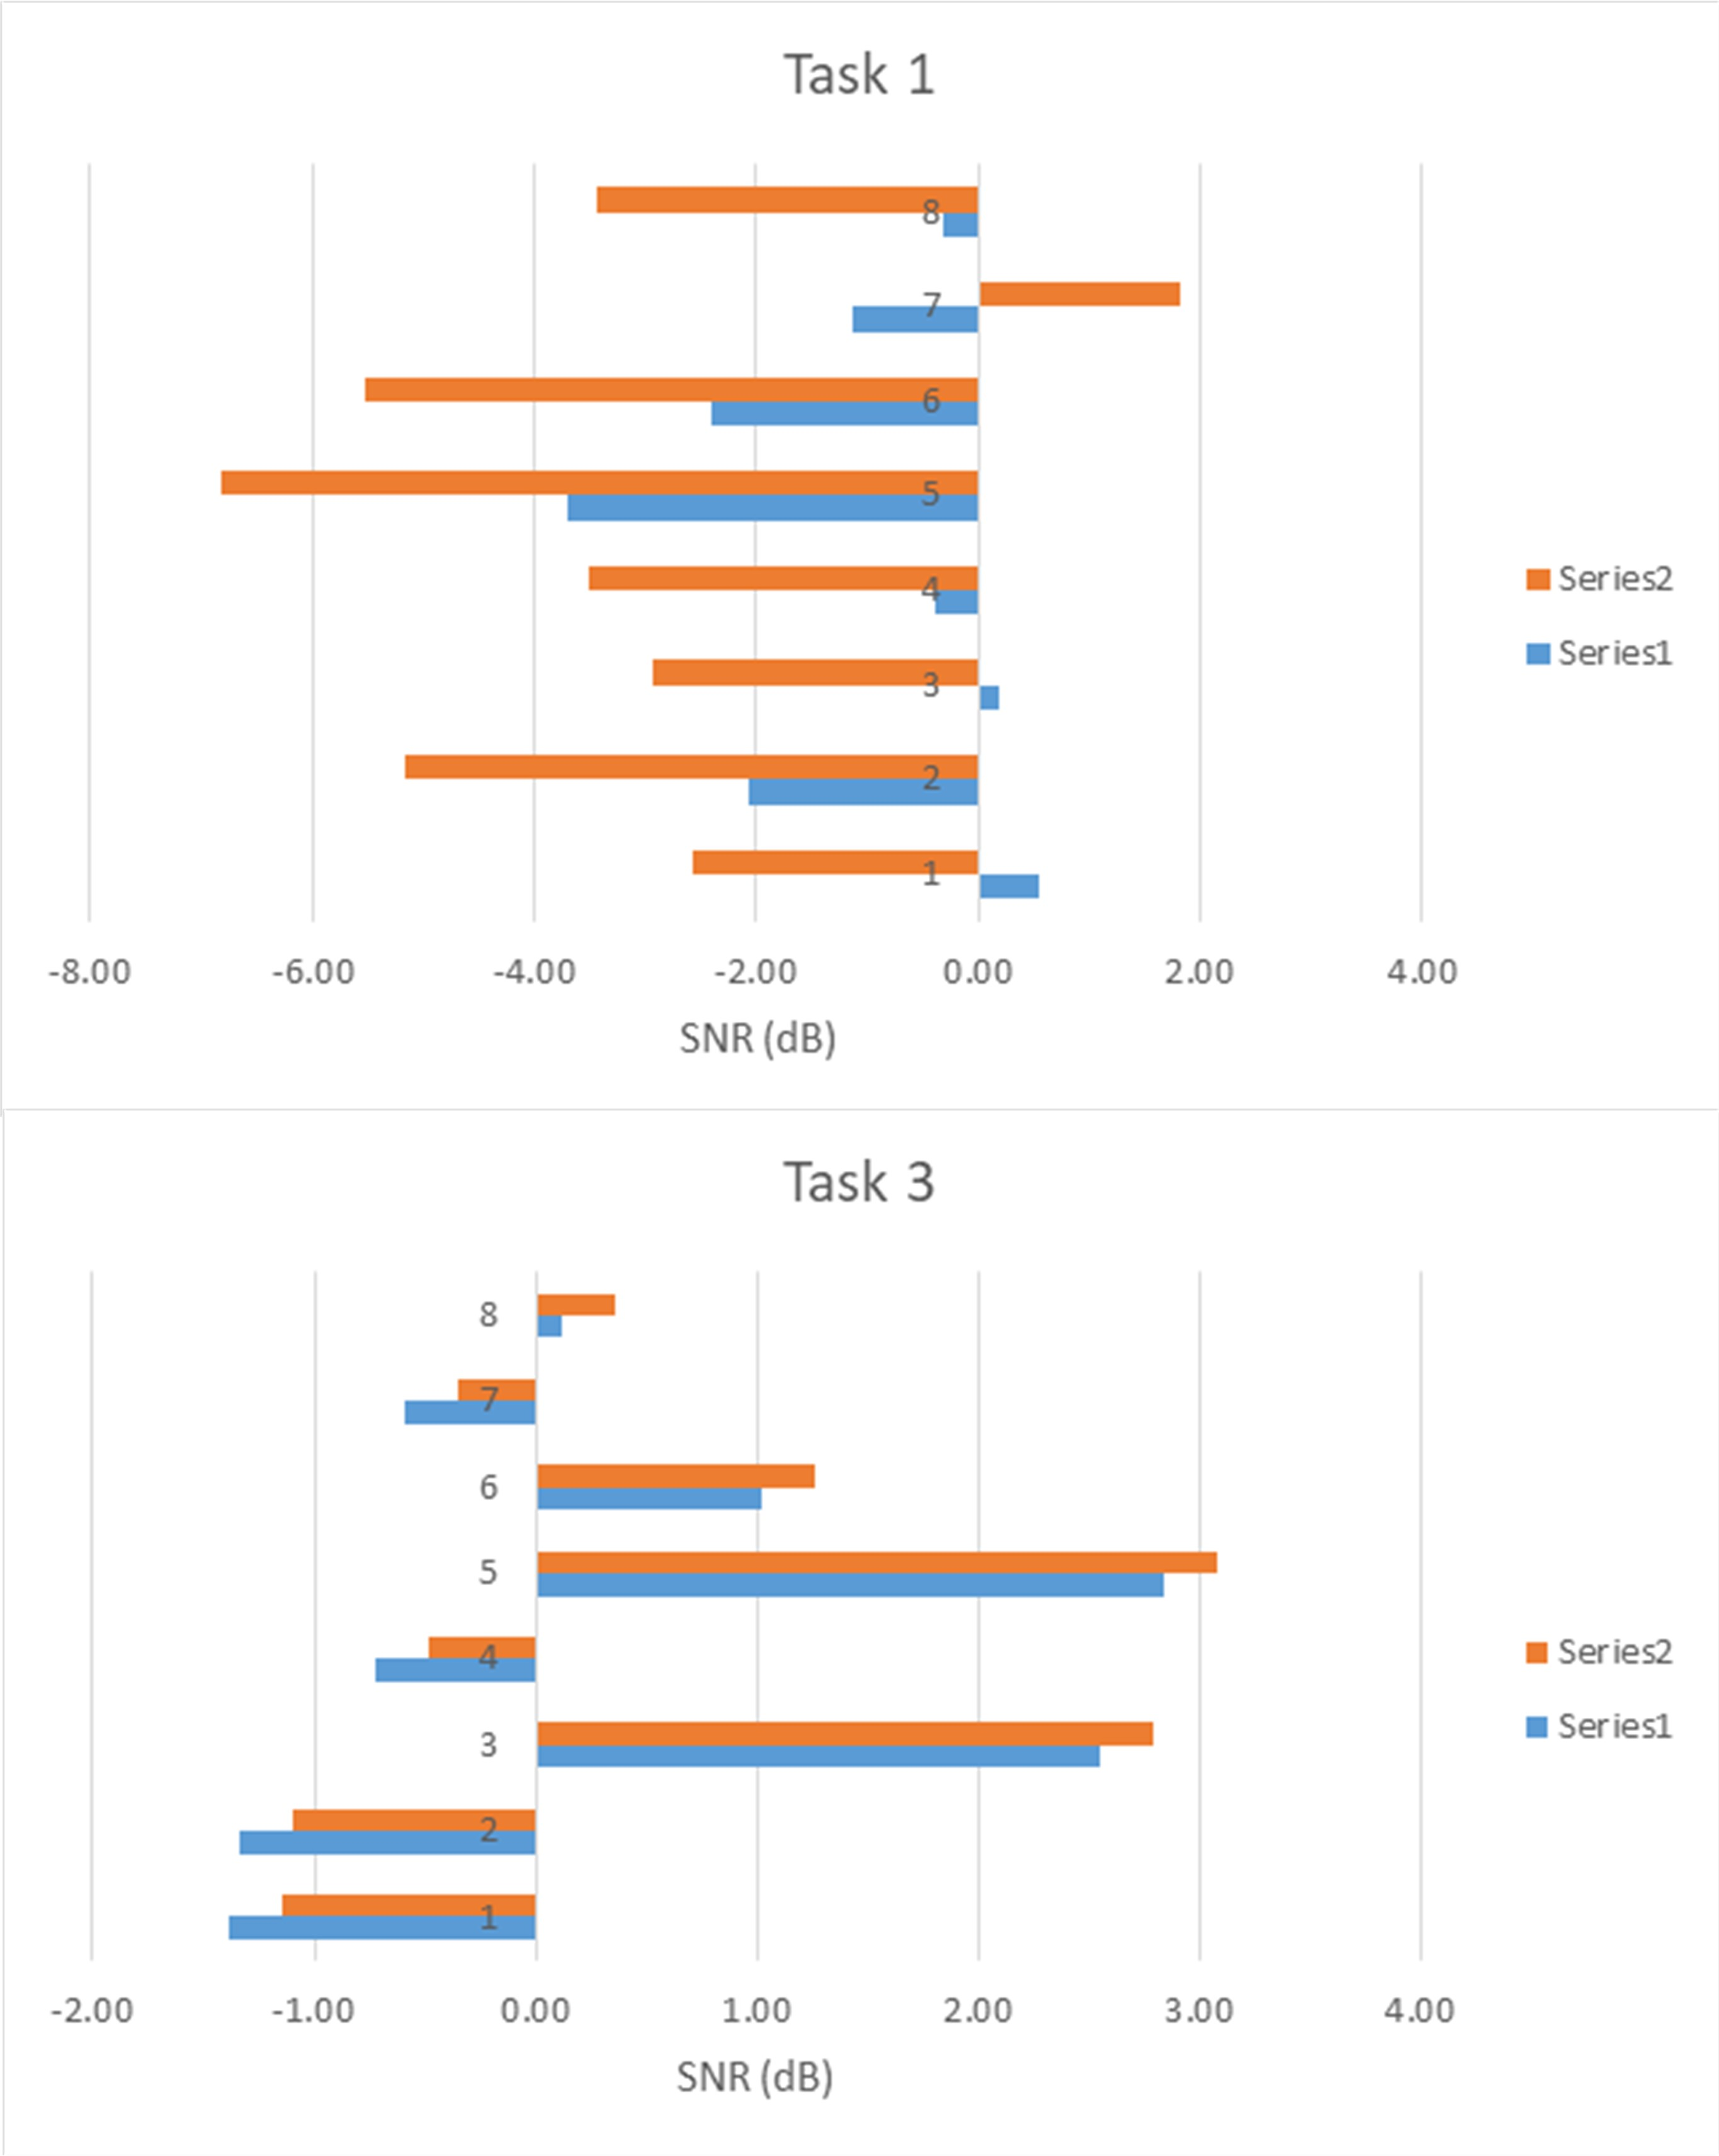
\includegraphics[width=\linewidth]{Figures/SNRchange.jpg} 
	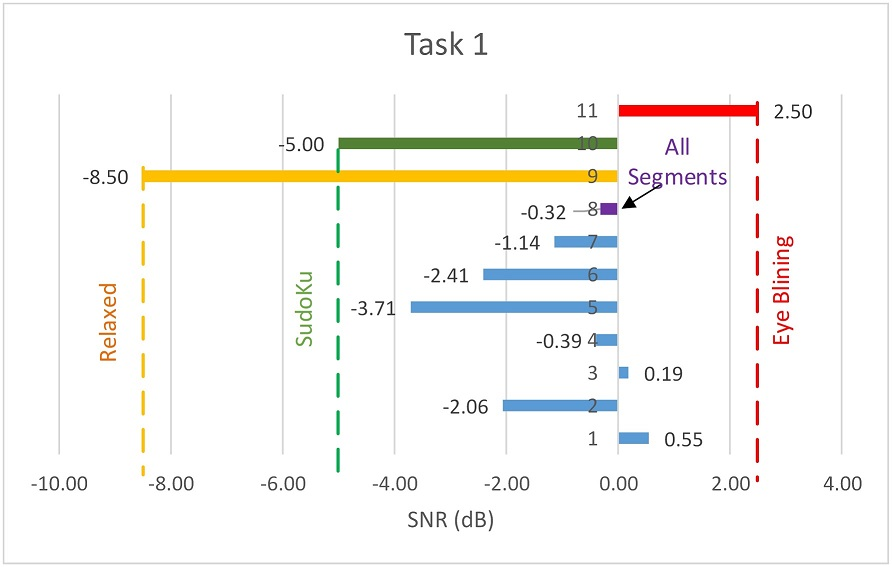
\includegraphics[width=10cm]{Figures/SNRtask1.jpg} 
	\caption{SNR for Task1.} 
	\label{SNR1} 
\end{figure}

\begin{figure}[hbt!]
	\centering
%	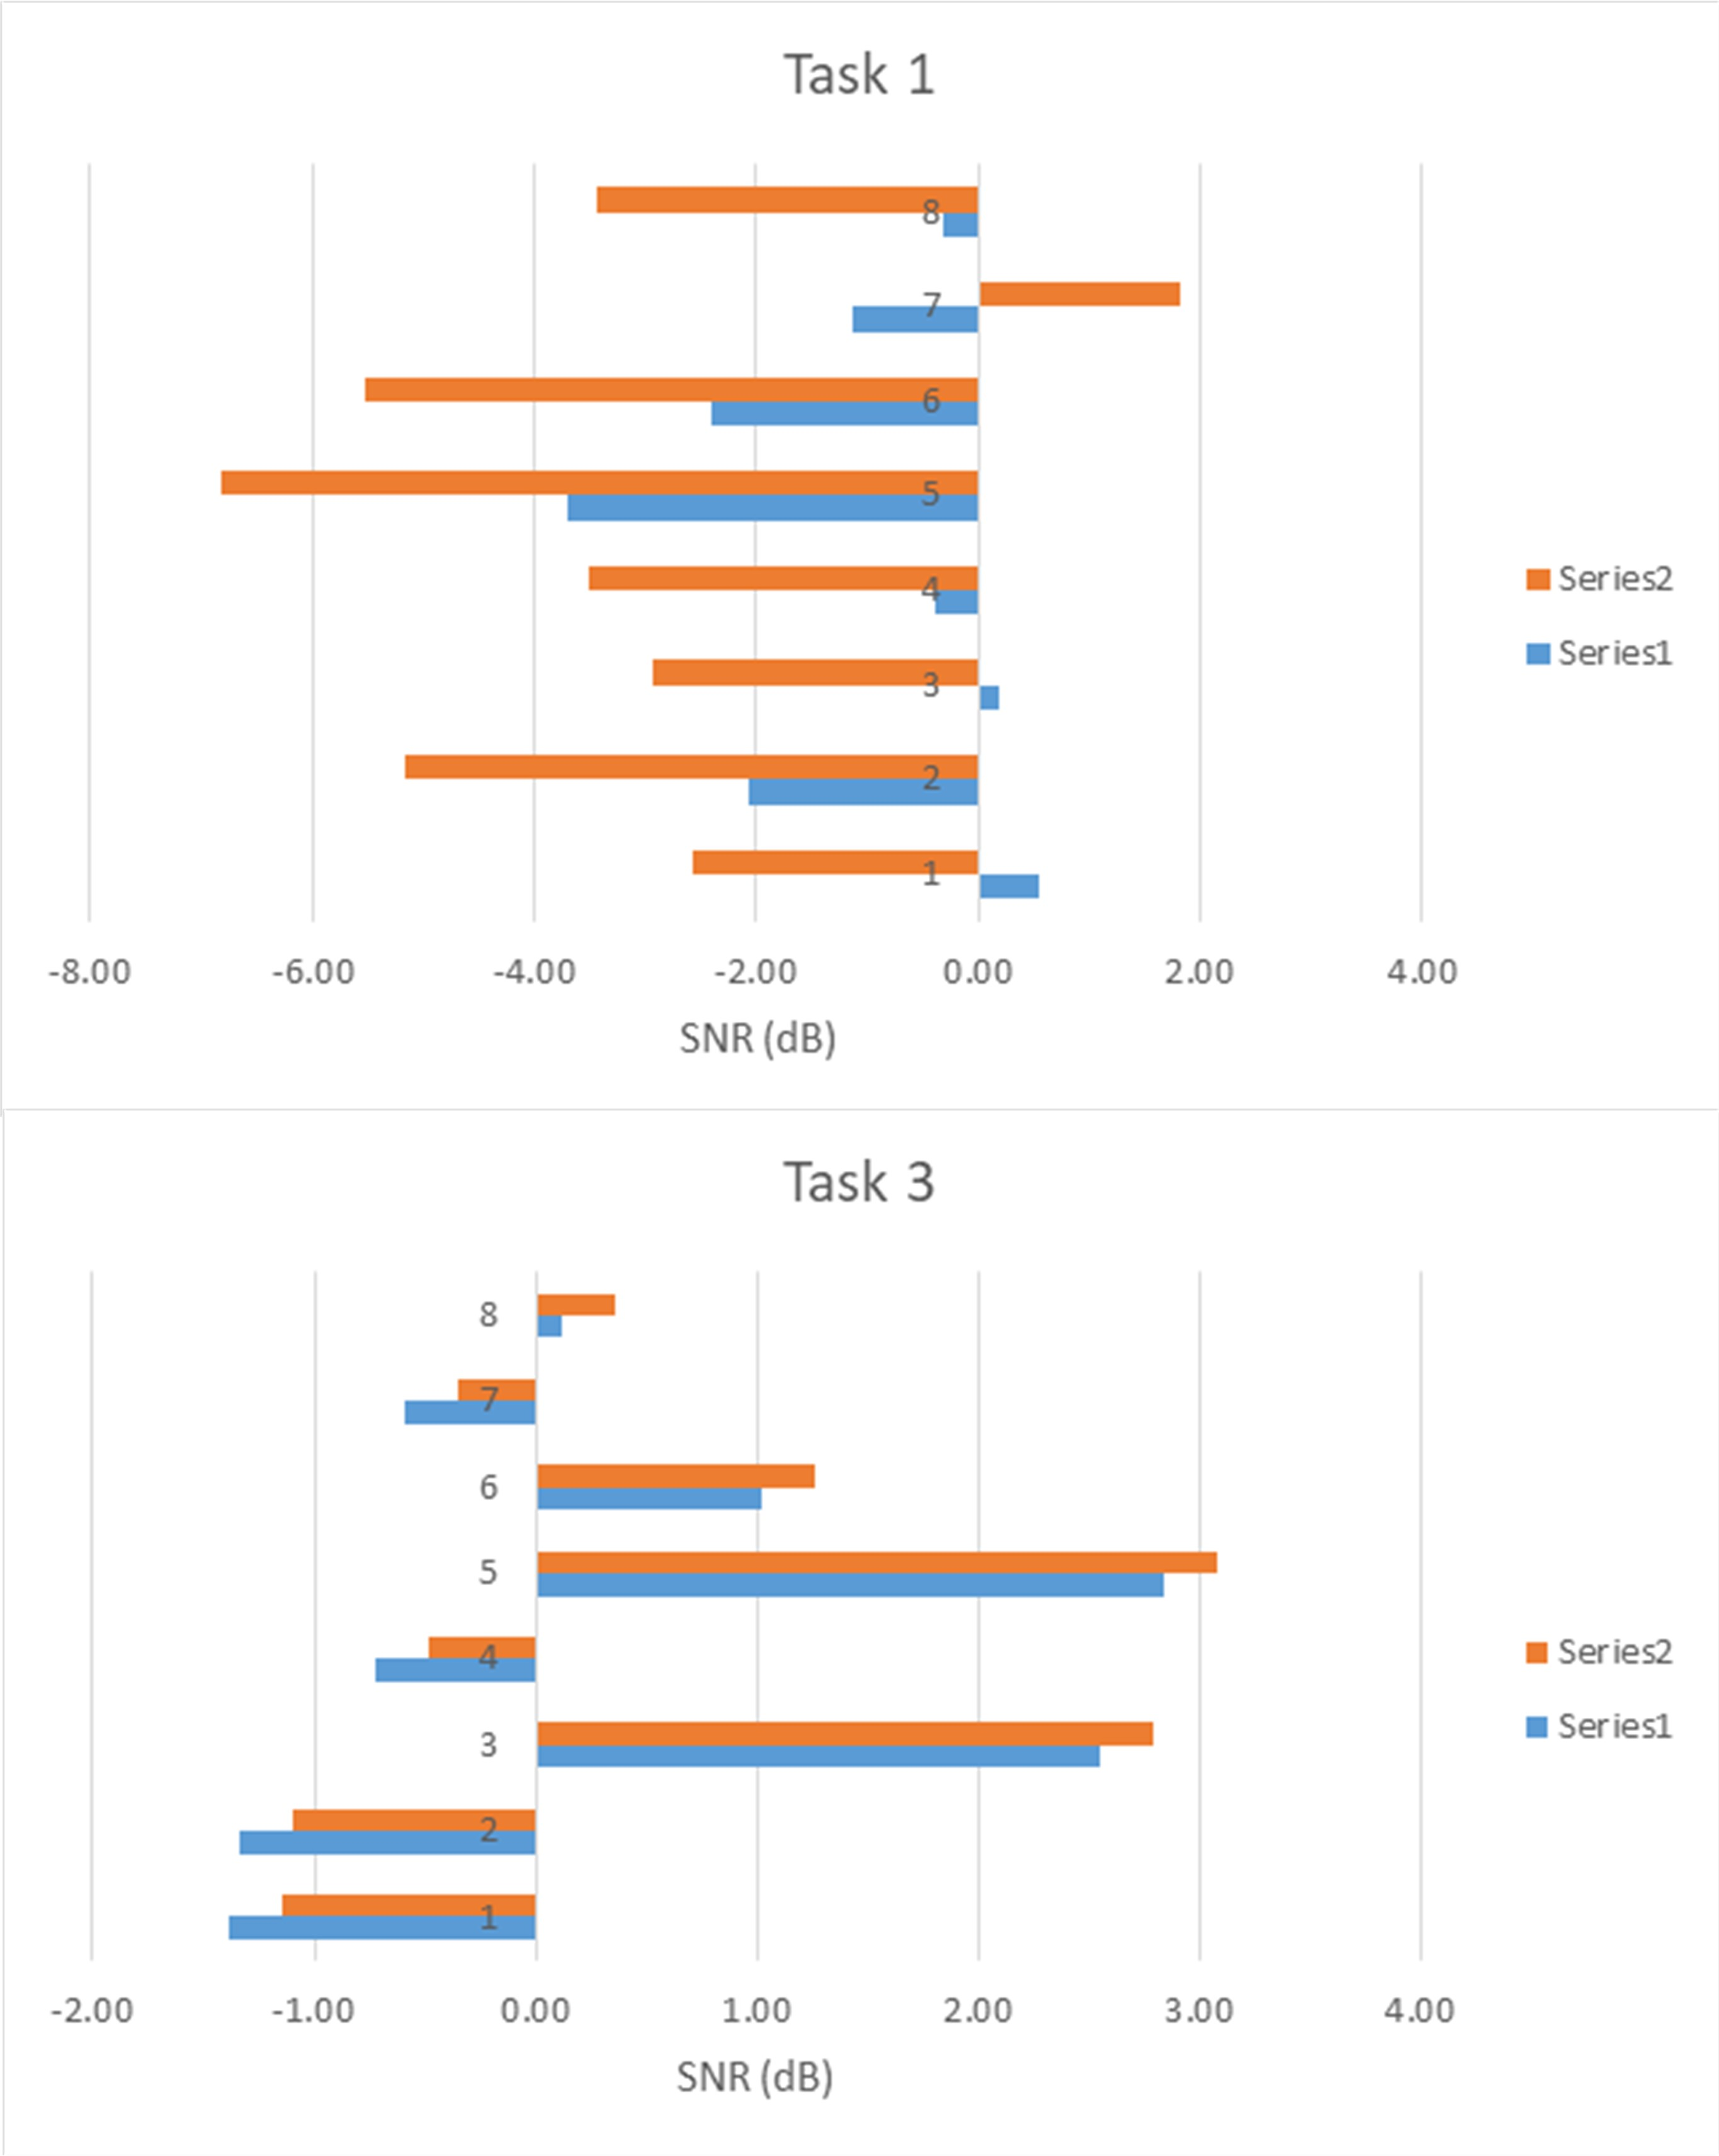
\includegraphics[width=\linewidth]{Figures/SNRchange.jpg} 
	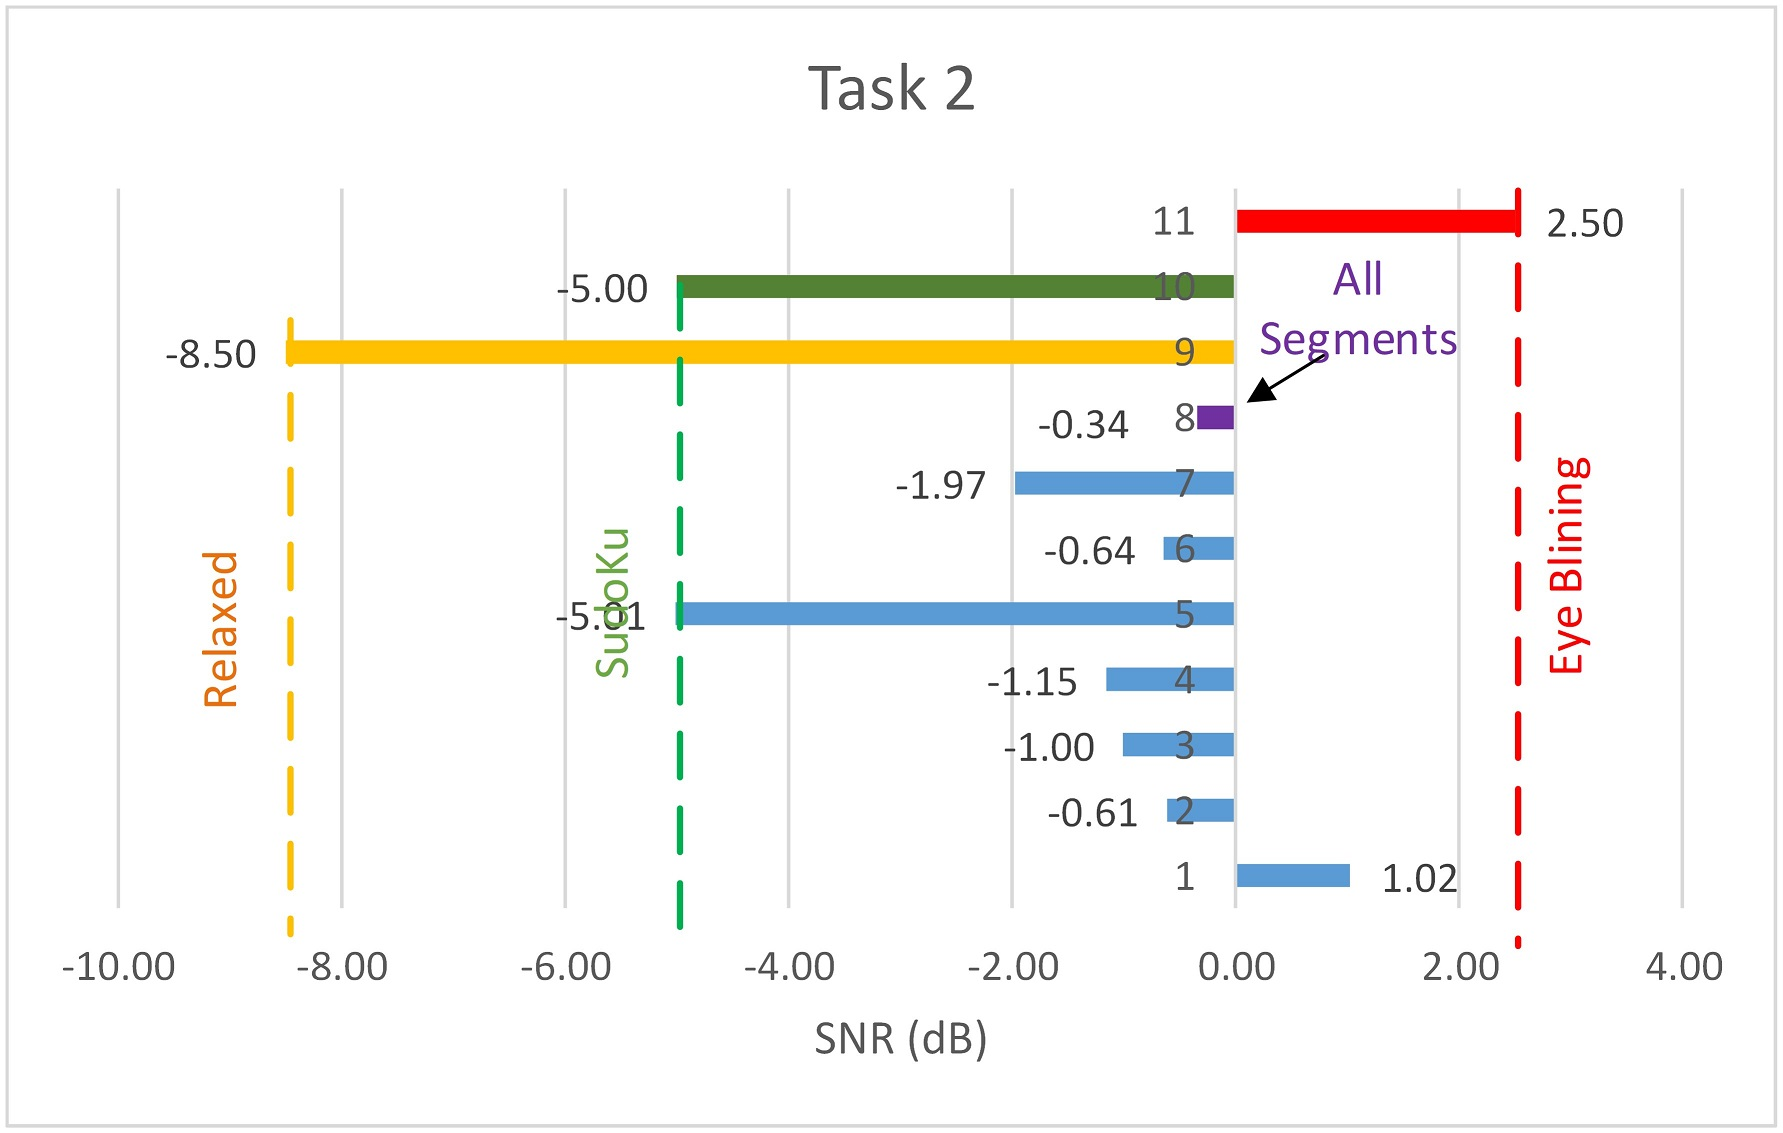
\includegraphics[width=10cm]{Figures/SNRtask2.jpg} 
	\caption{SNR for Task2.} 
	\label{SNR2} 
\end{figure}

\begin{figure}[hbt!]
	\centering
%	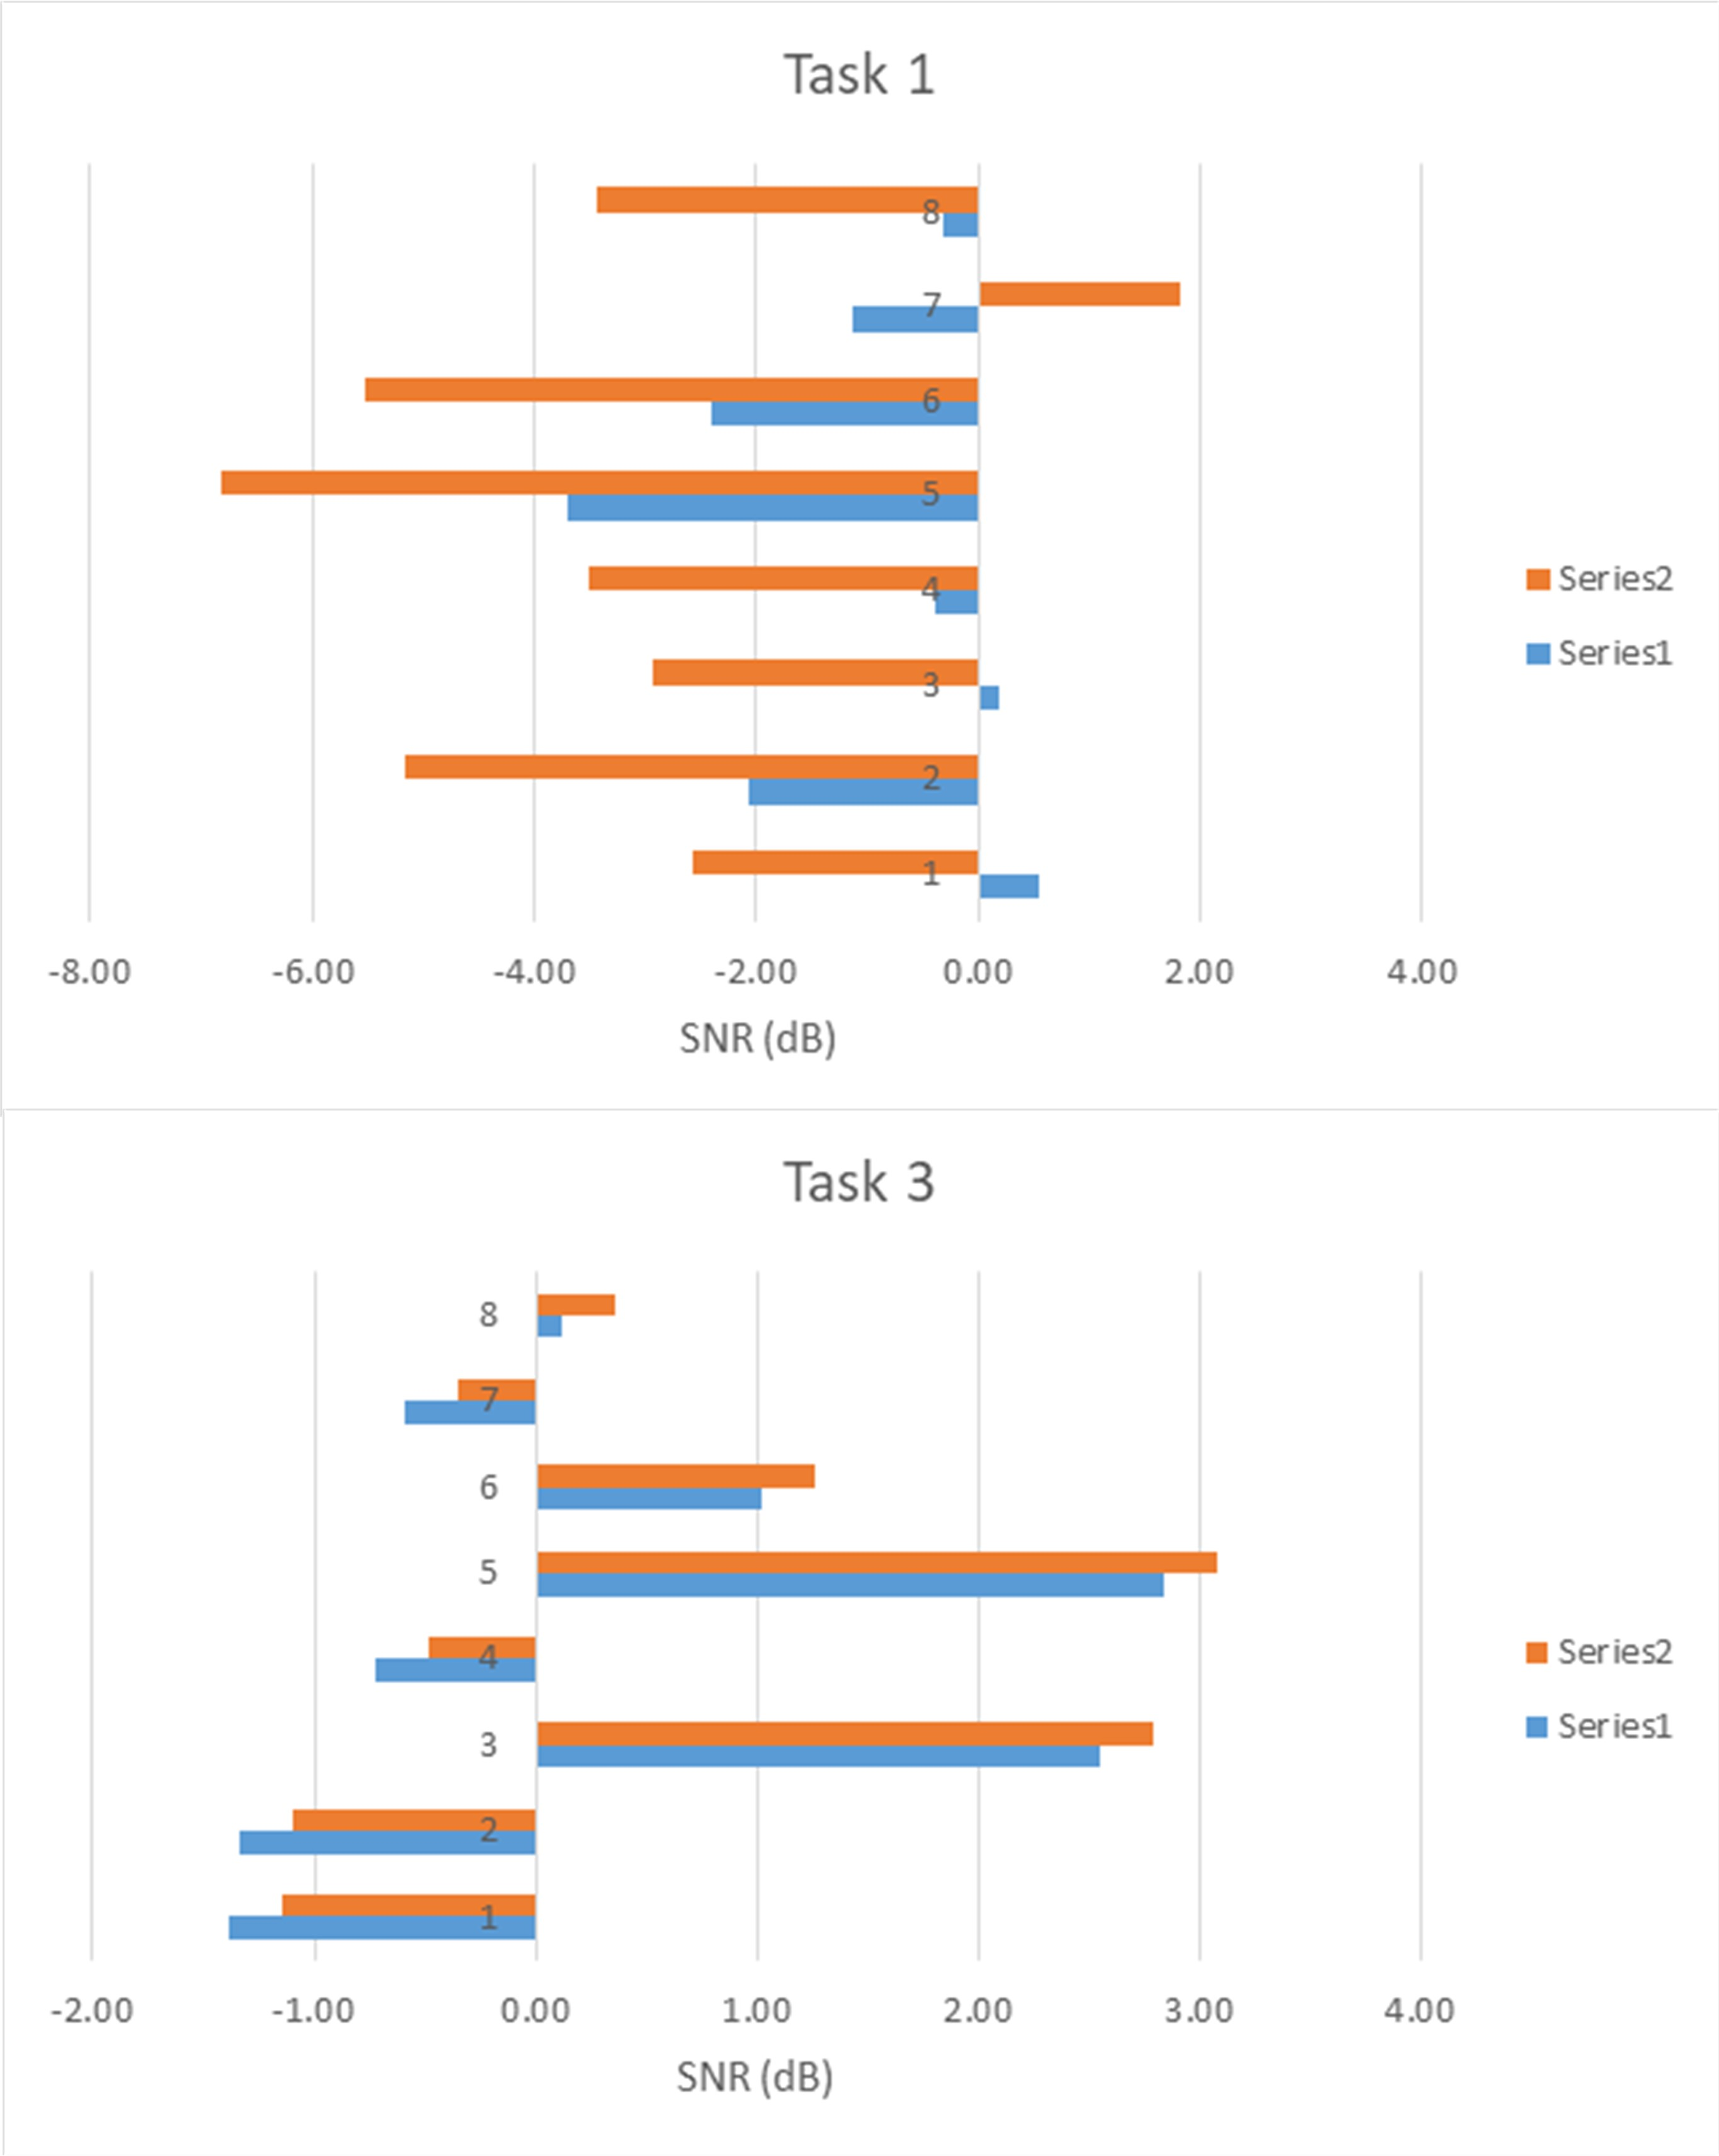
\includegraphics[width=\linewidth]{Figures/SNRchange.jpg} 
	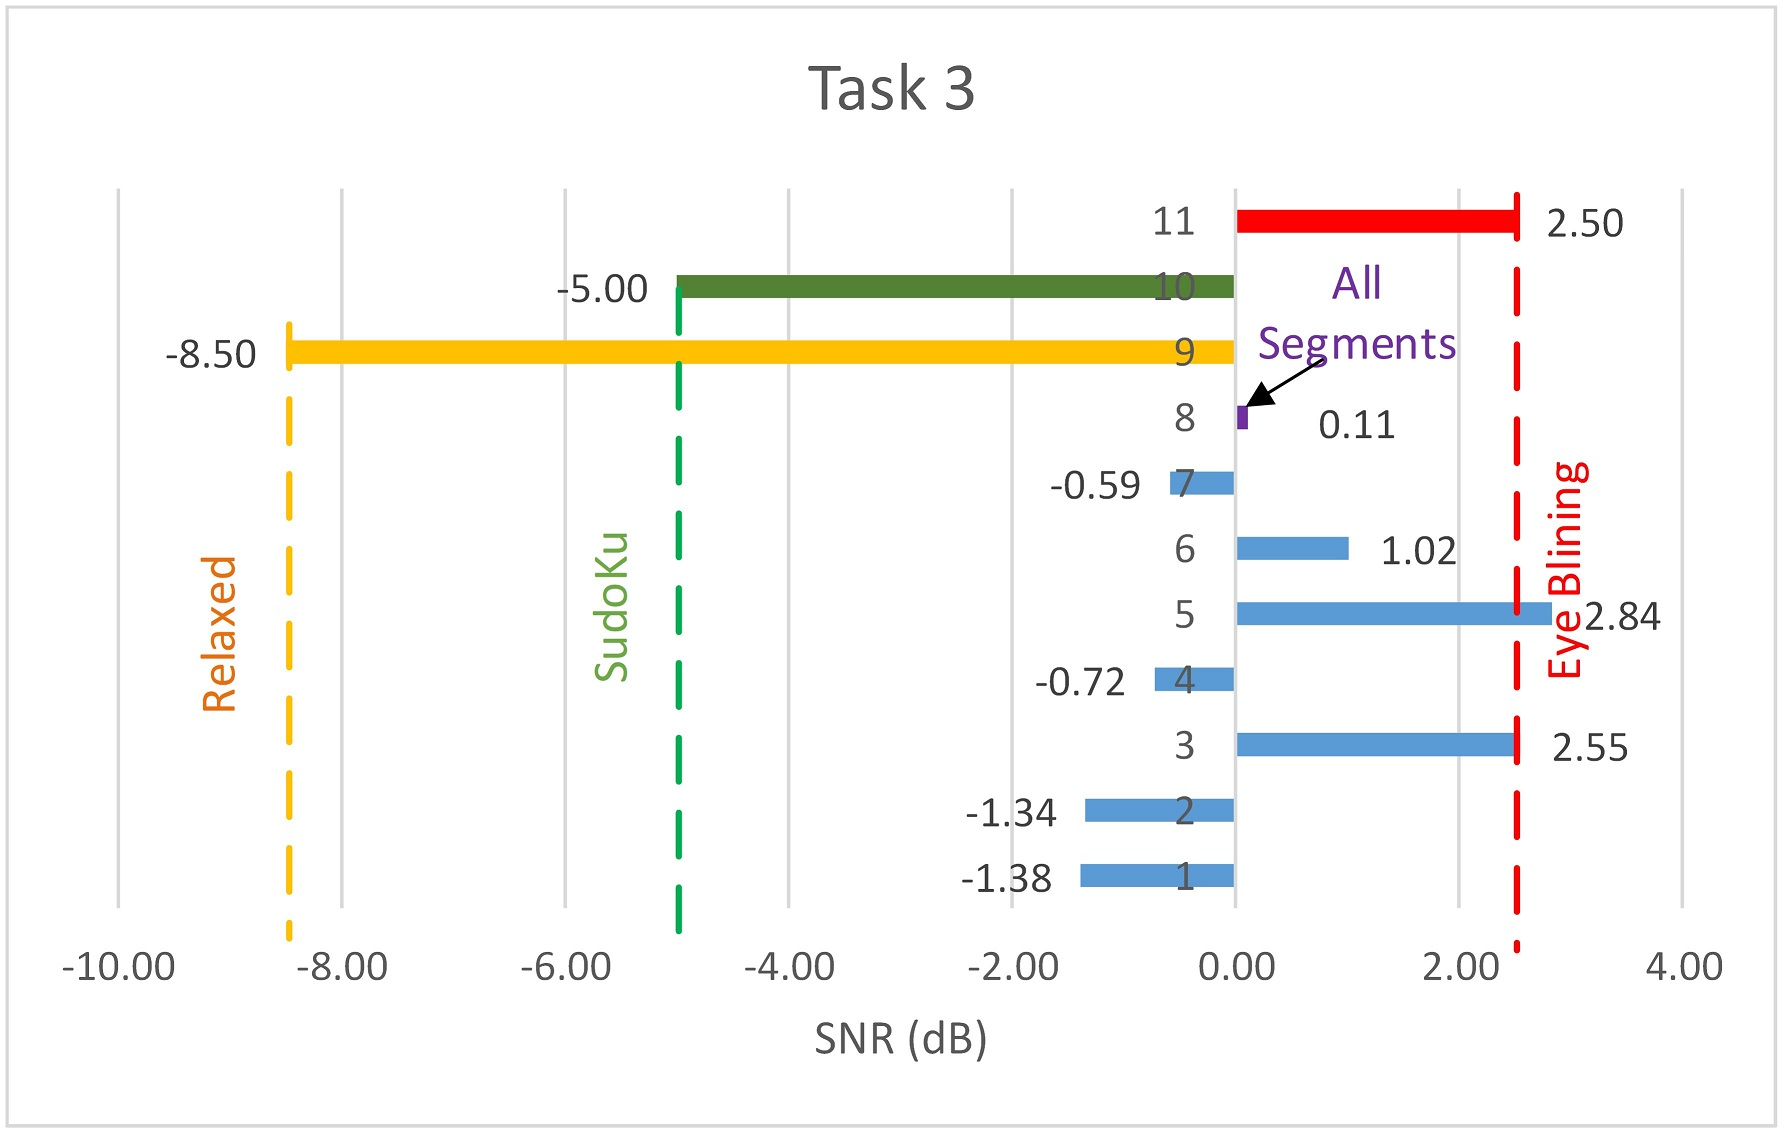
\includegraphics[width=10cm]{Figures/SNRtask3.jpg} 
	\caption{SNR for Task3.} 
	\label{SNR3} 
\end{figure}


\begin{figure}[hbt!]
	\centering
%	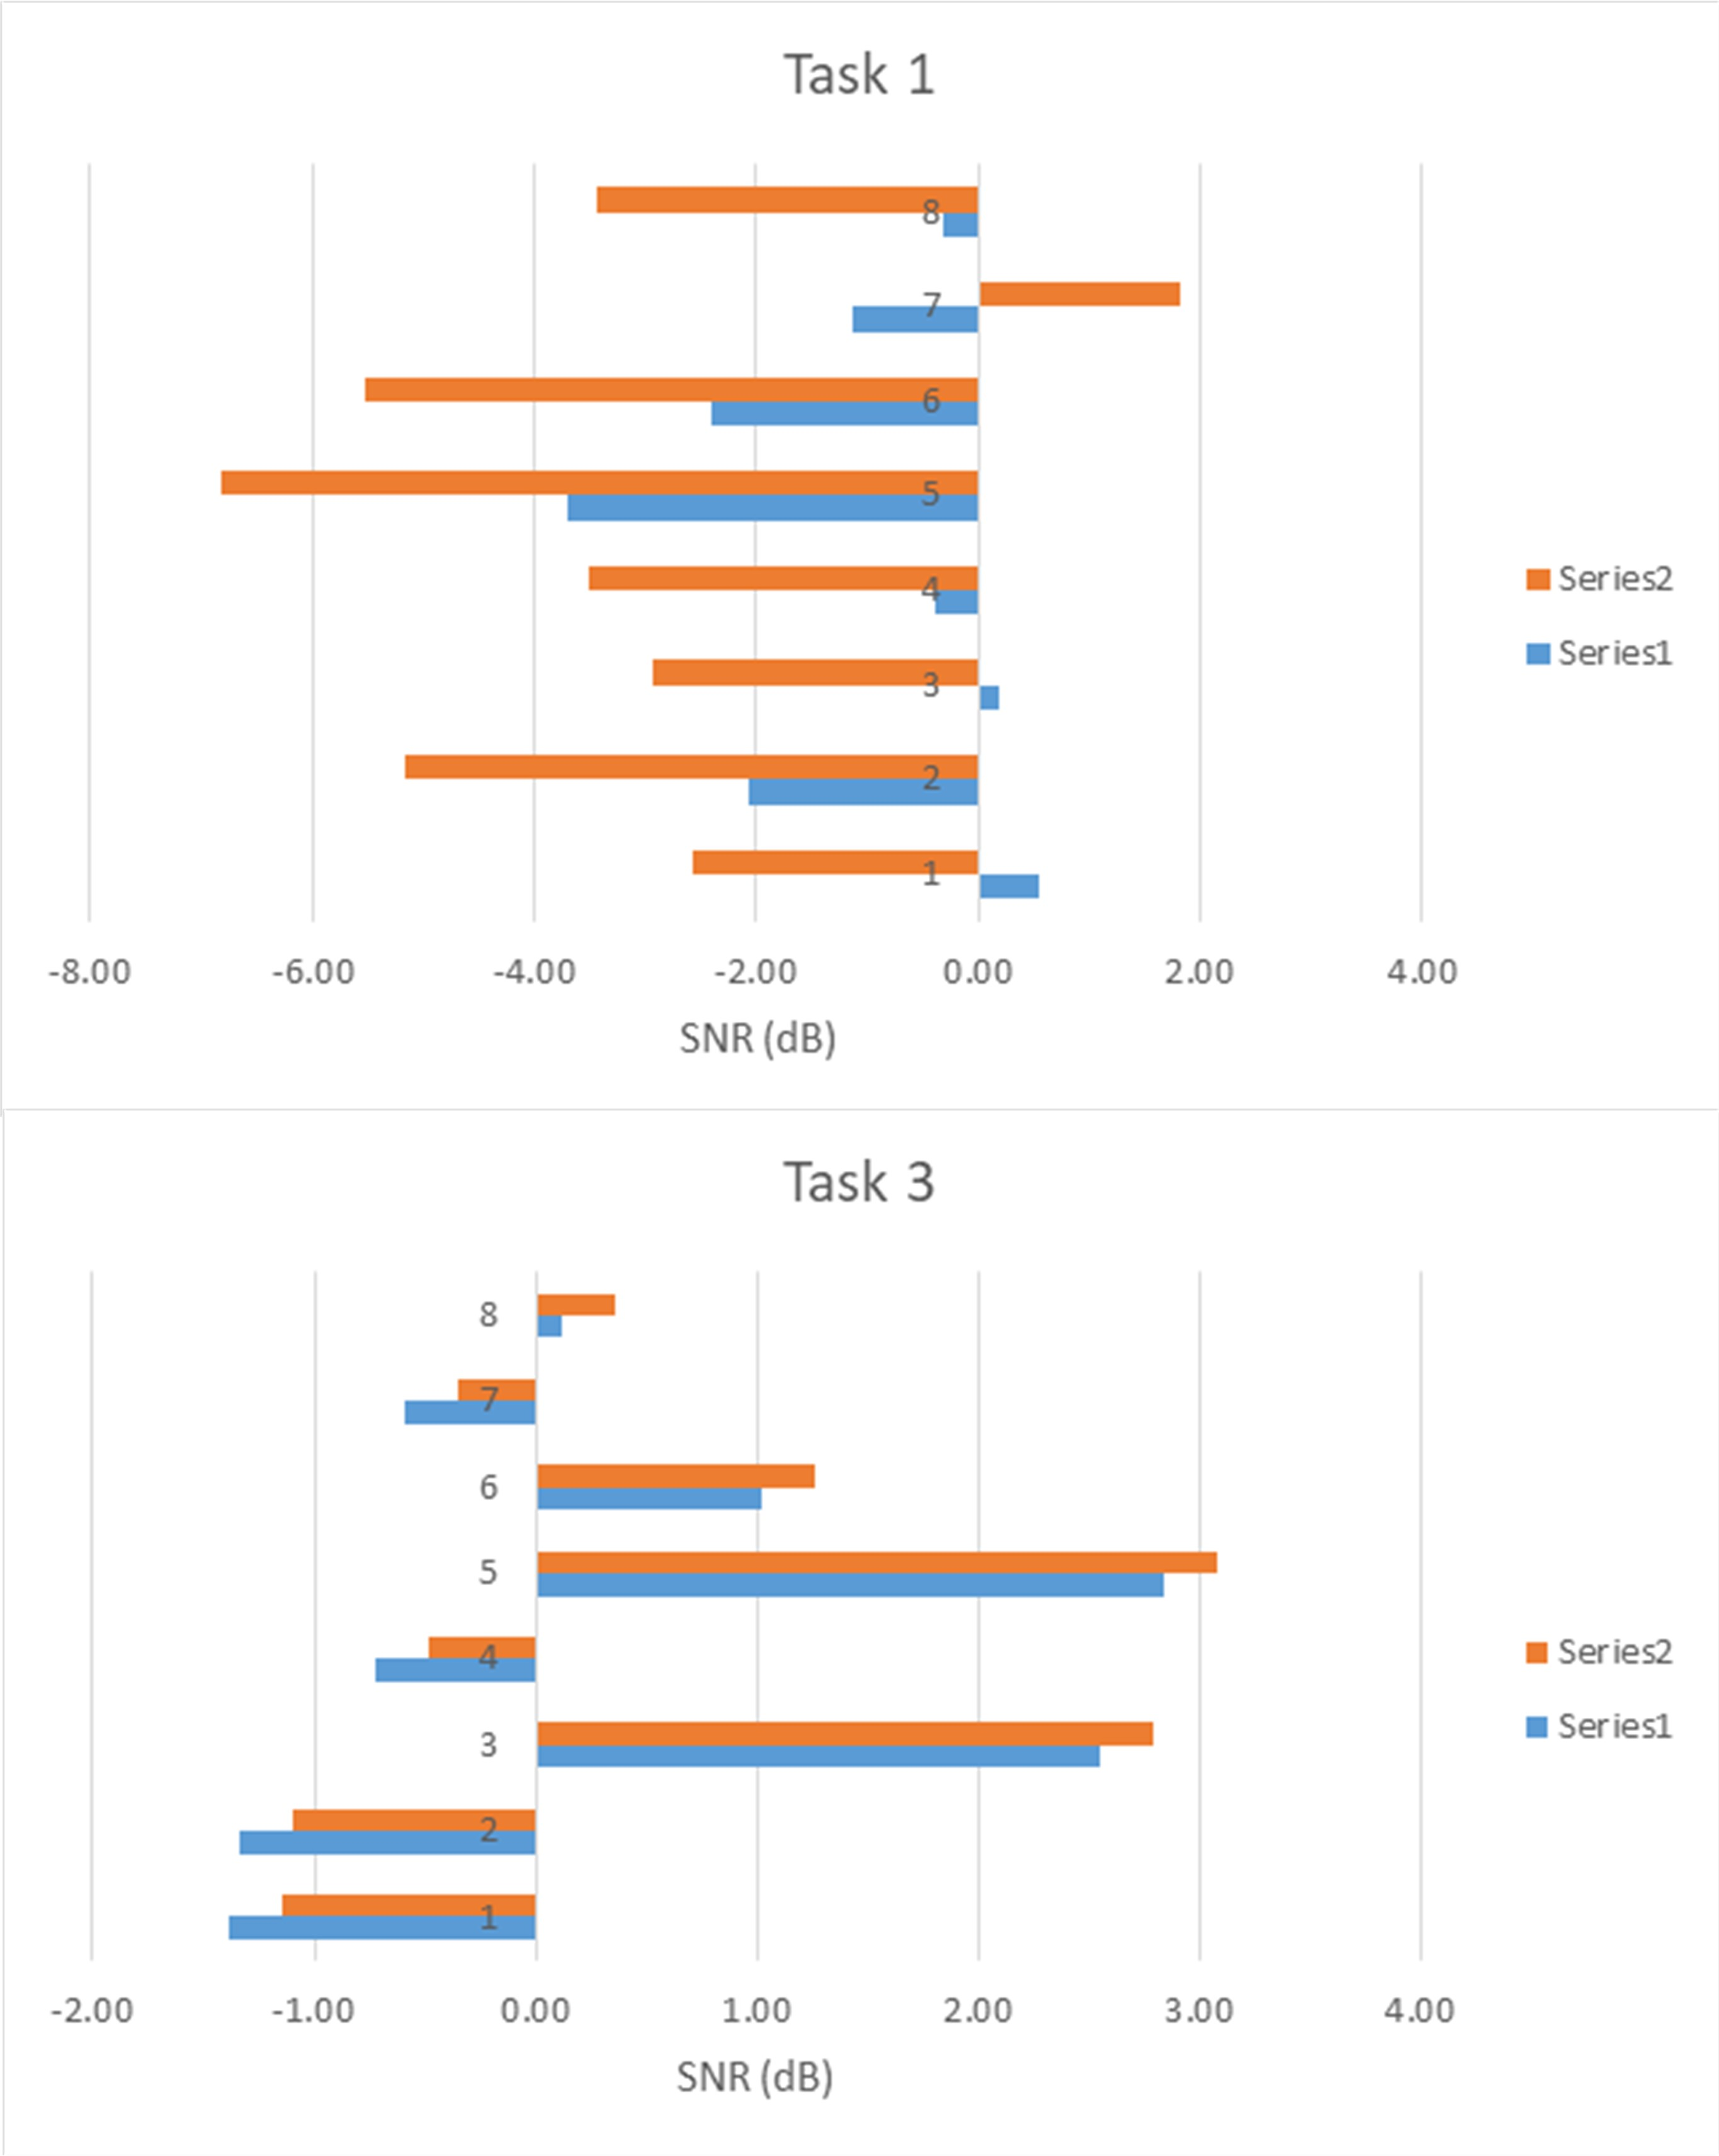
\includegraphics[width=\linewidth]{Figures/SNRchange.jpg} 
	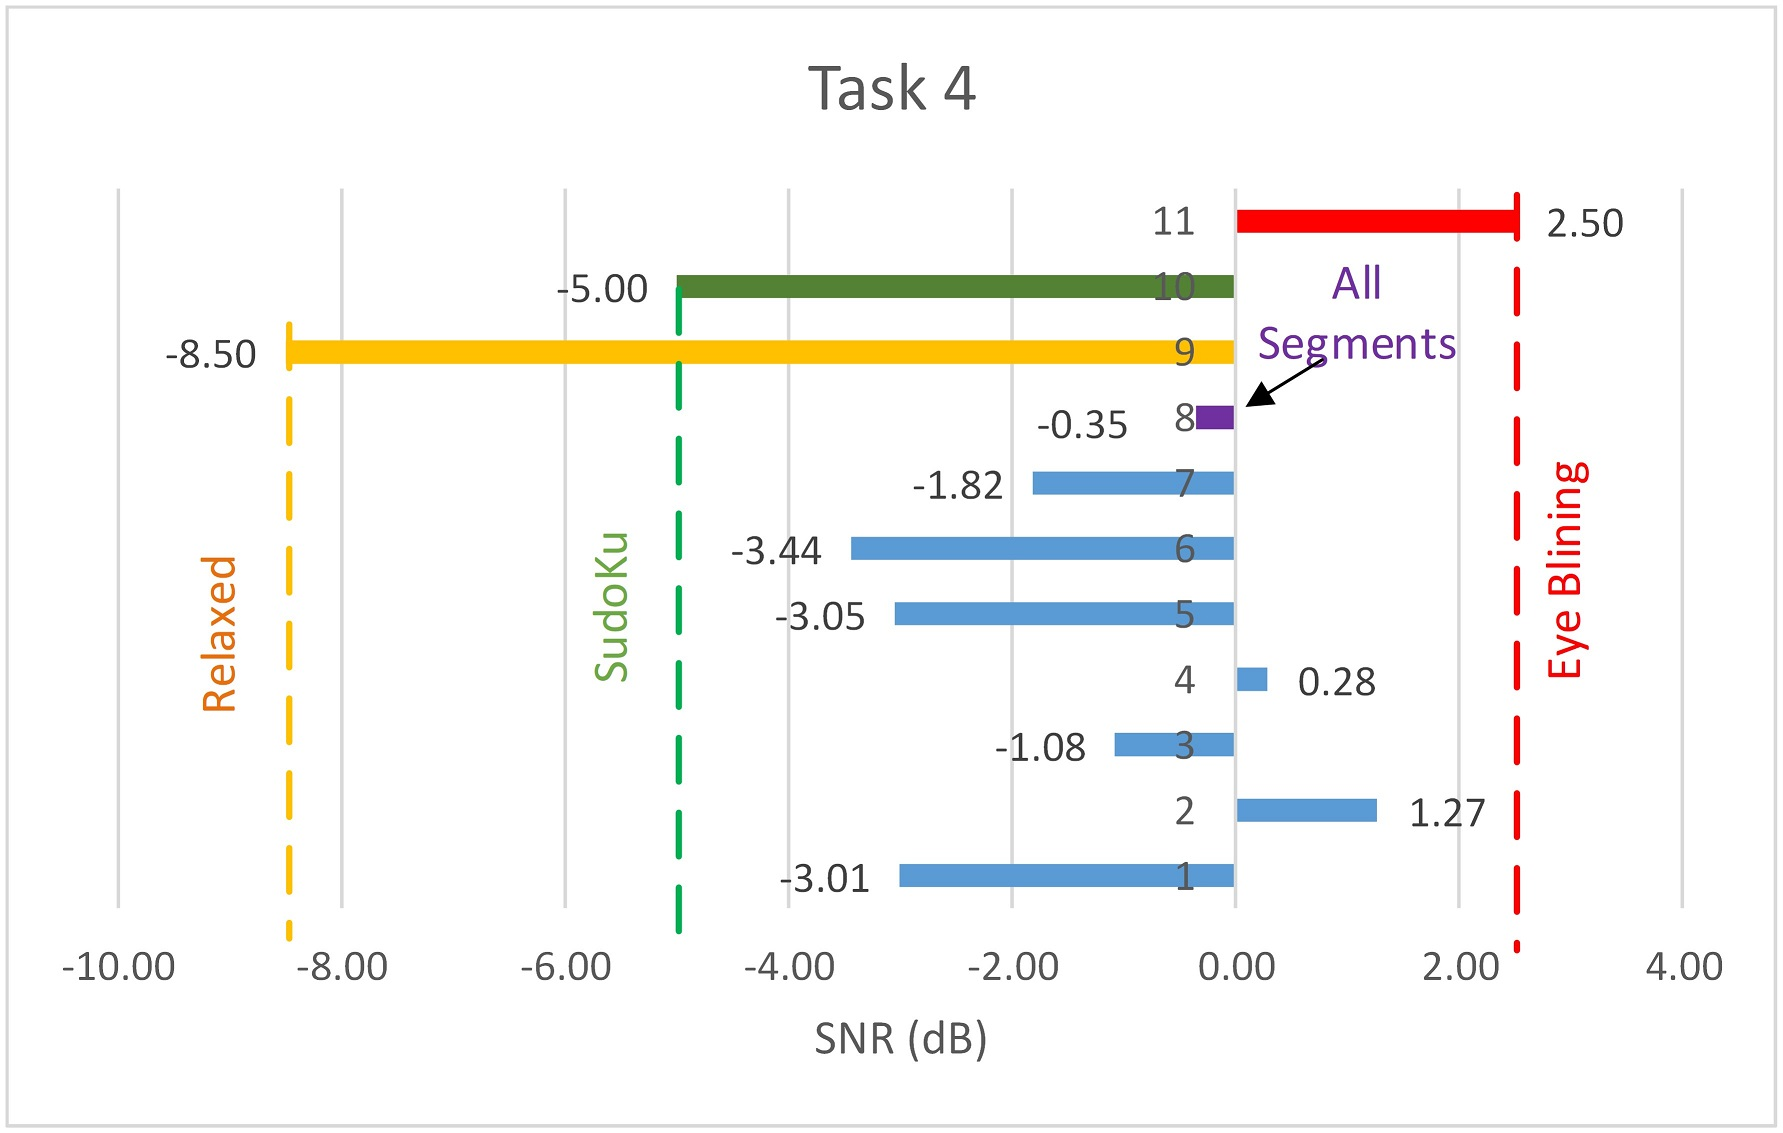
\includegraphics[width=10cm]{Figures/SNRtask4.jpg} 
	\caption{SNR for Task4.} 
	\label{SNR4} 
\end{figure}


\begin{figure}[hbt!]
	\centering
%	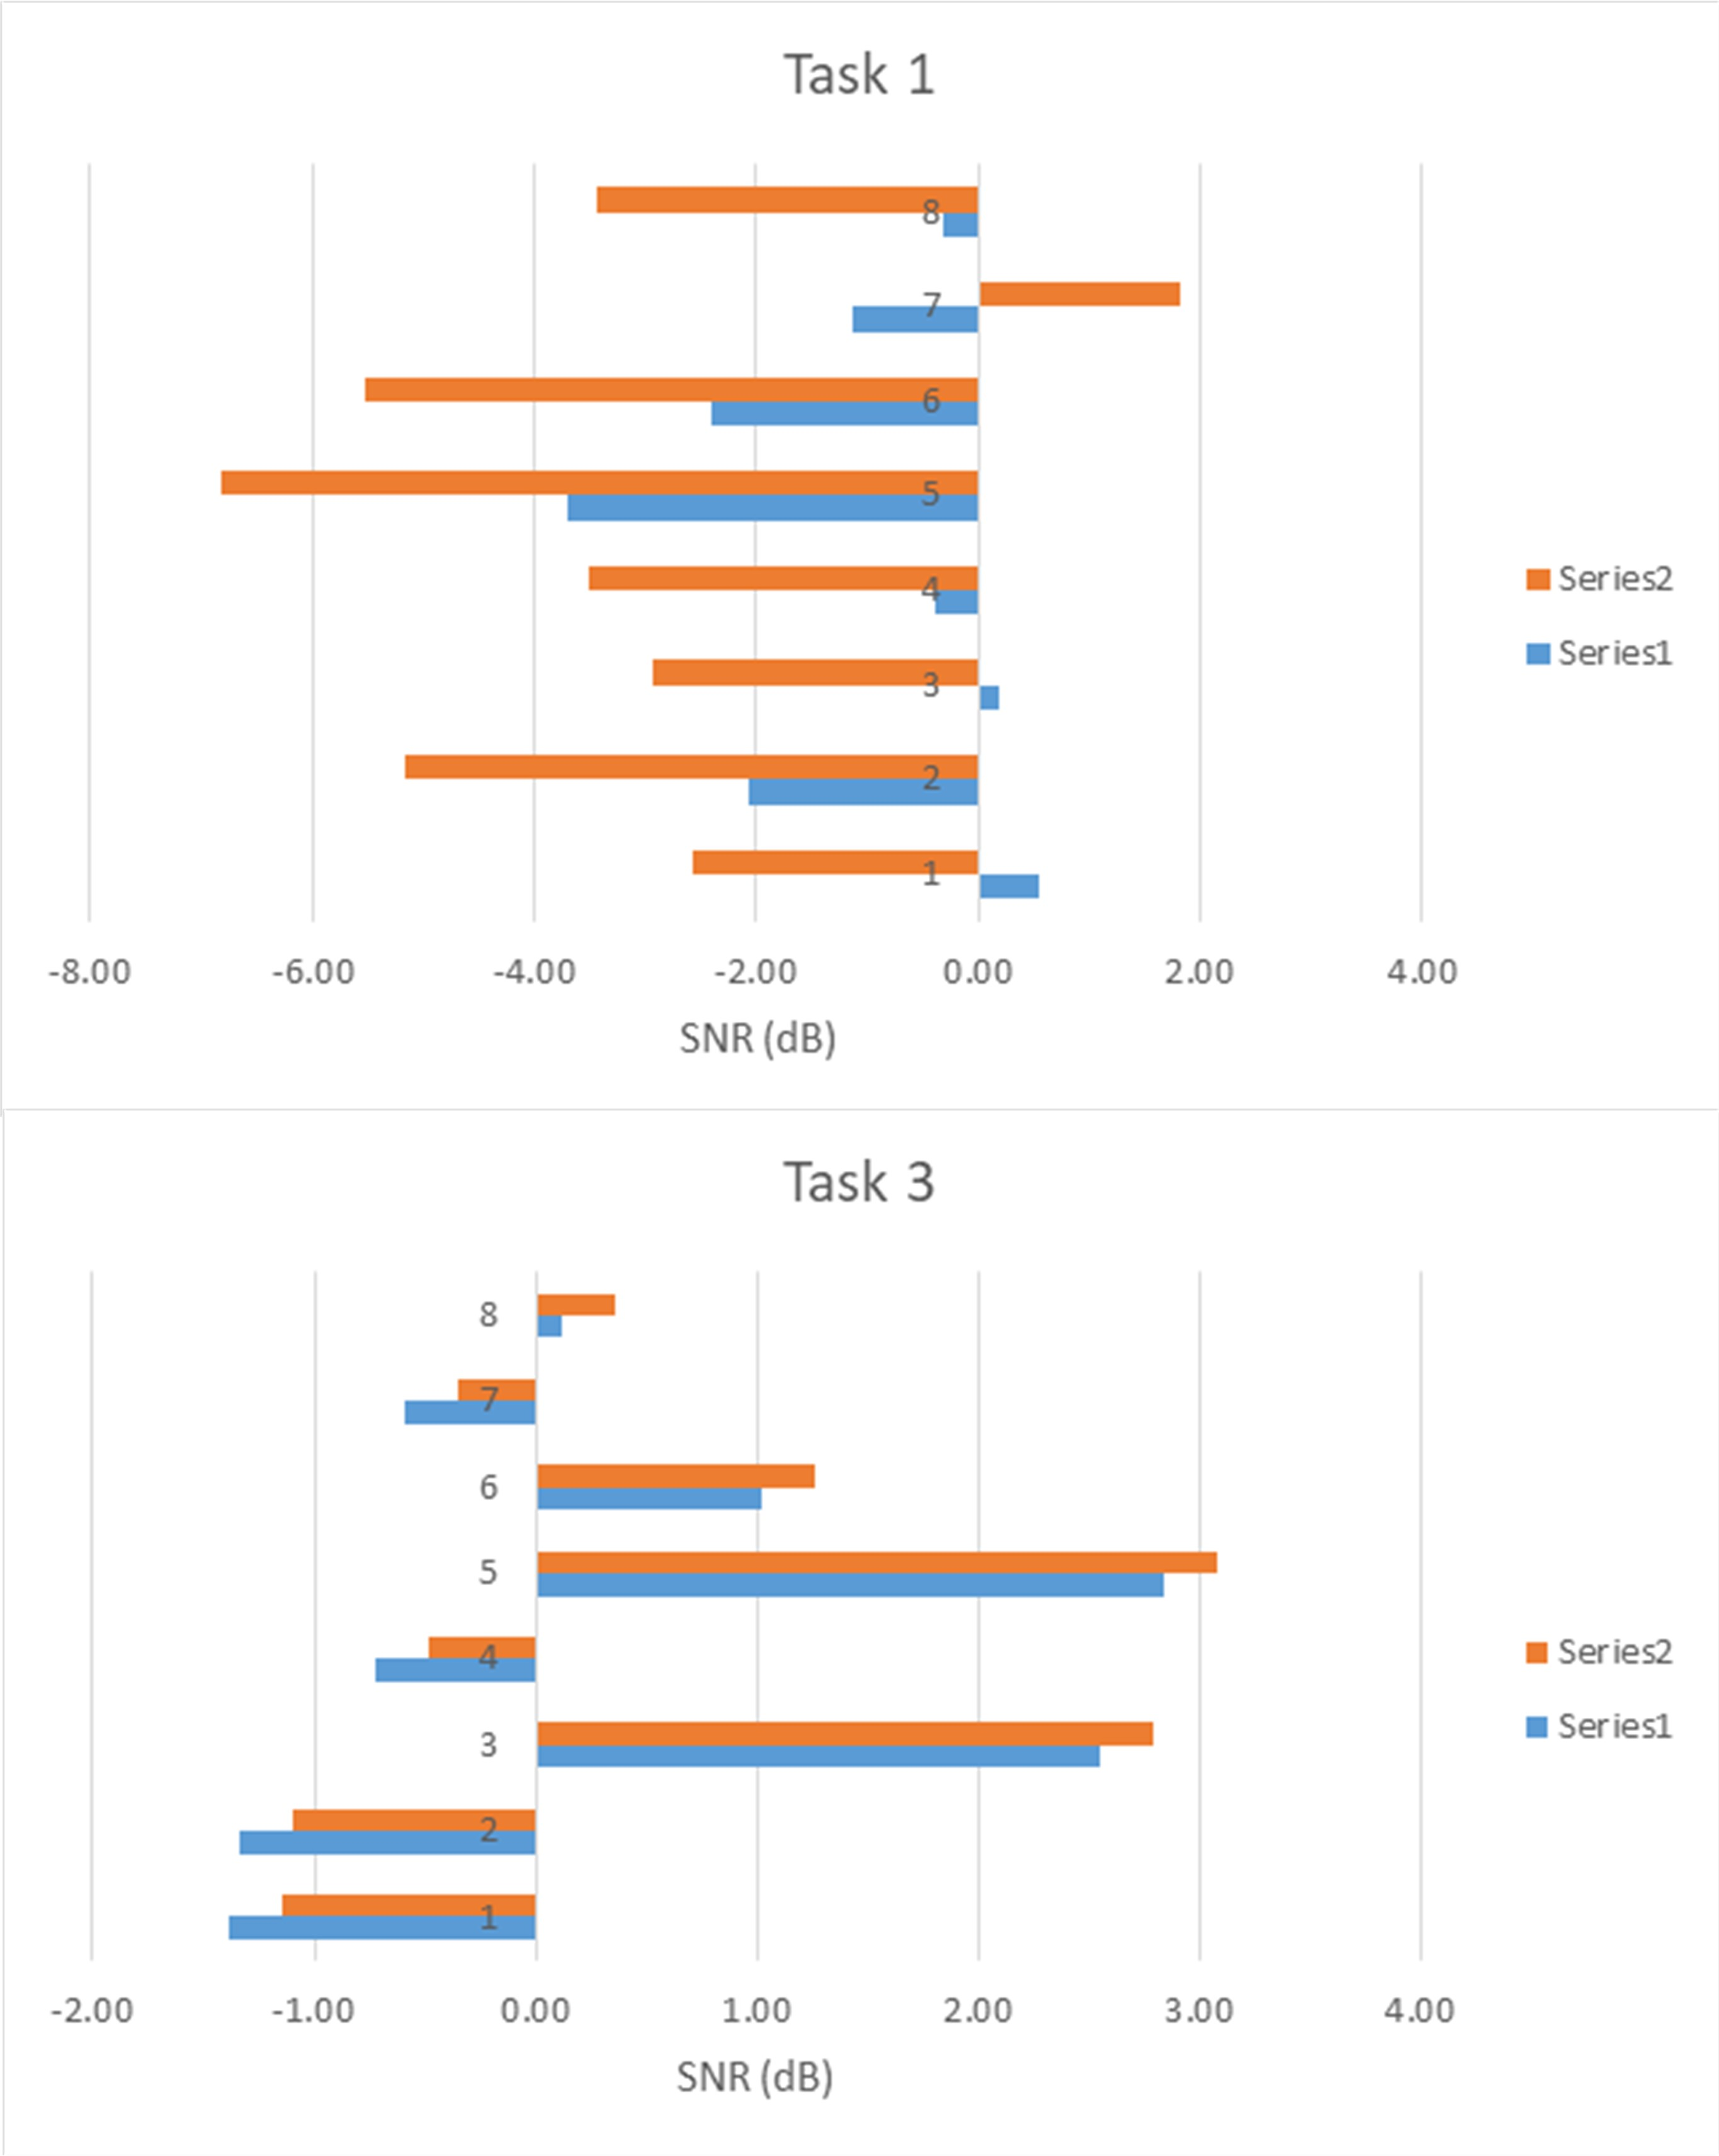
\includegraphics[width=\linewidth]{Figures/SNRchange.jpg} 
	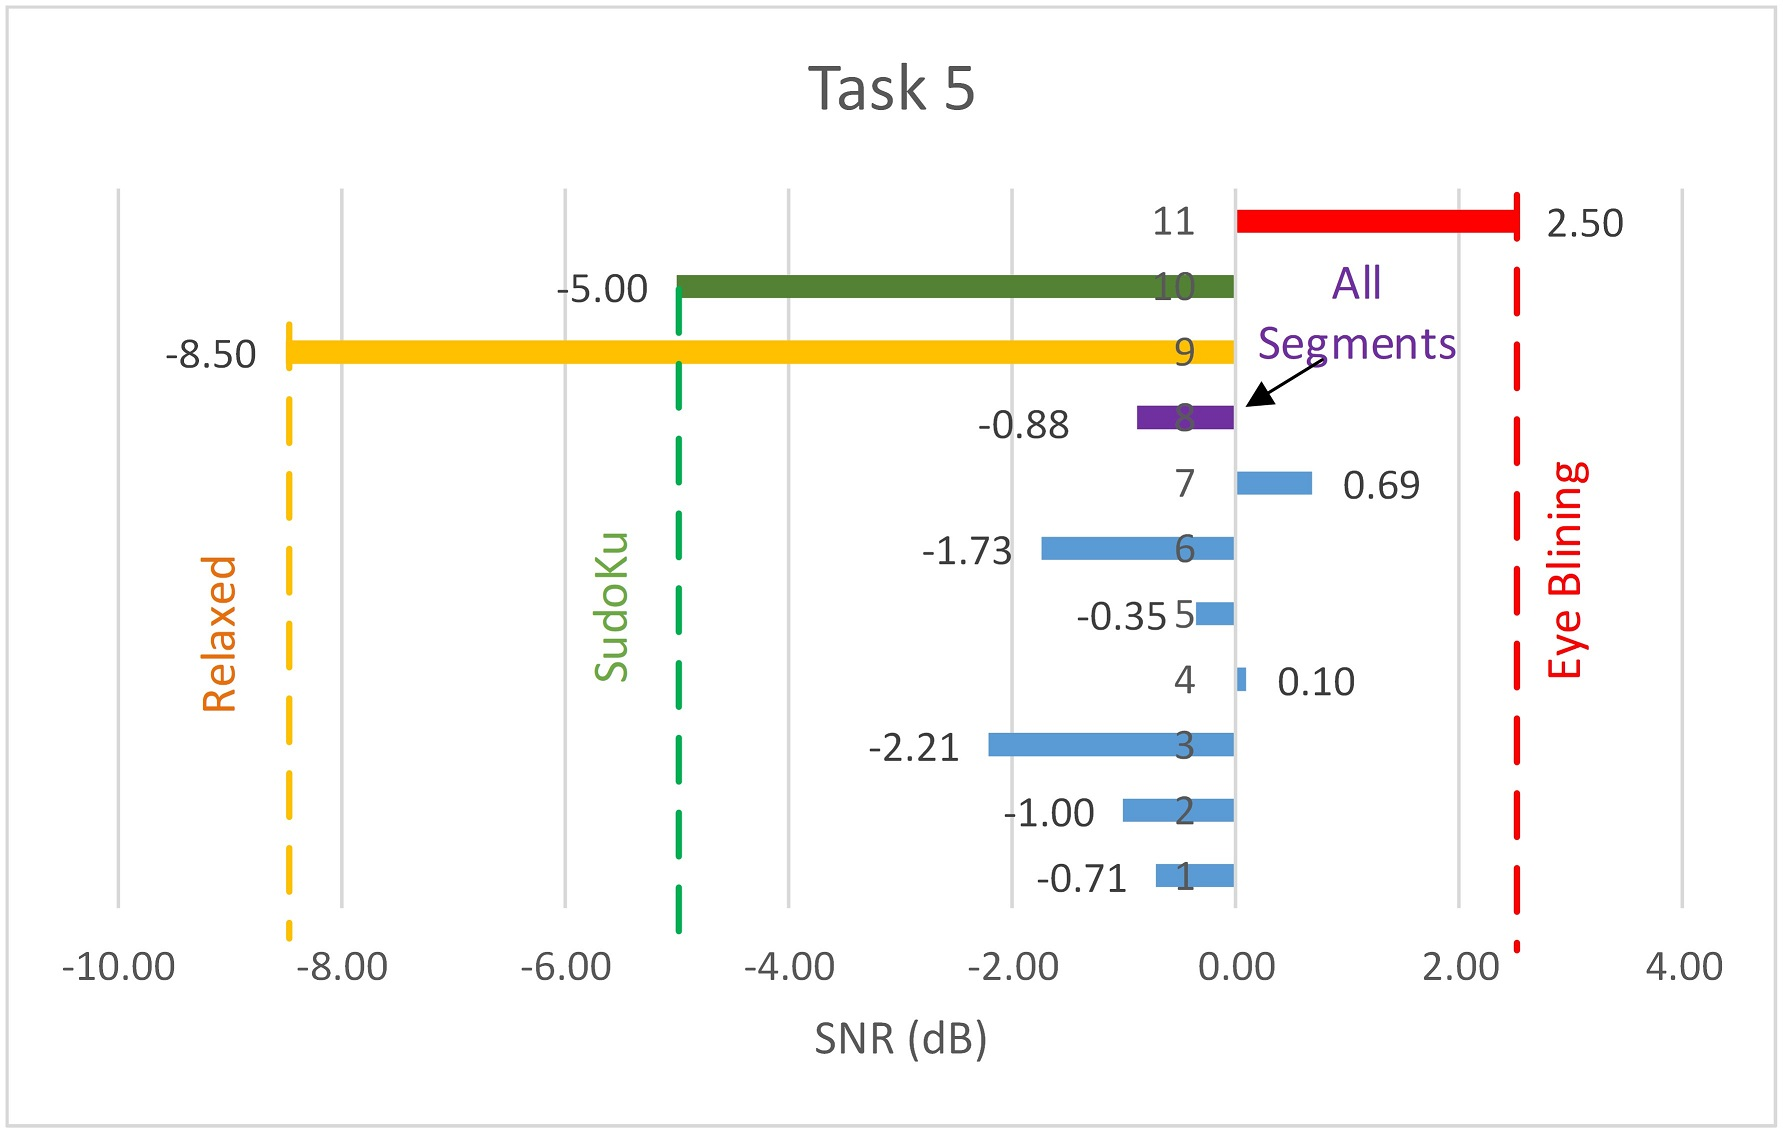
\includegraphics[width=10cm]{Figures/SNRtask5.jpg} 
	\caption{SNR for Task5.} 
	\label{SNR5} 
\end{figure}


\begin{figure}[hbt!]
	\centering
%	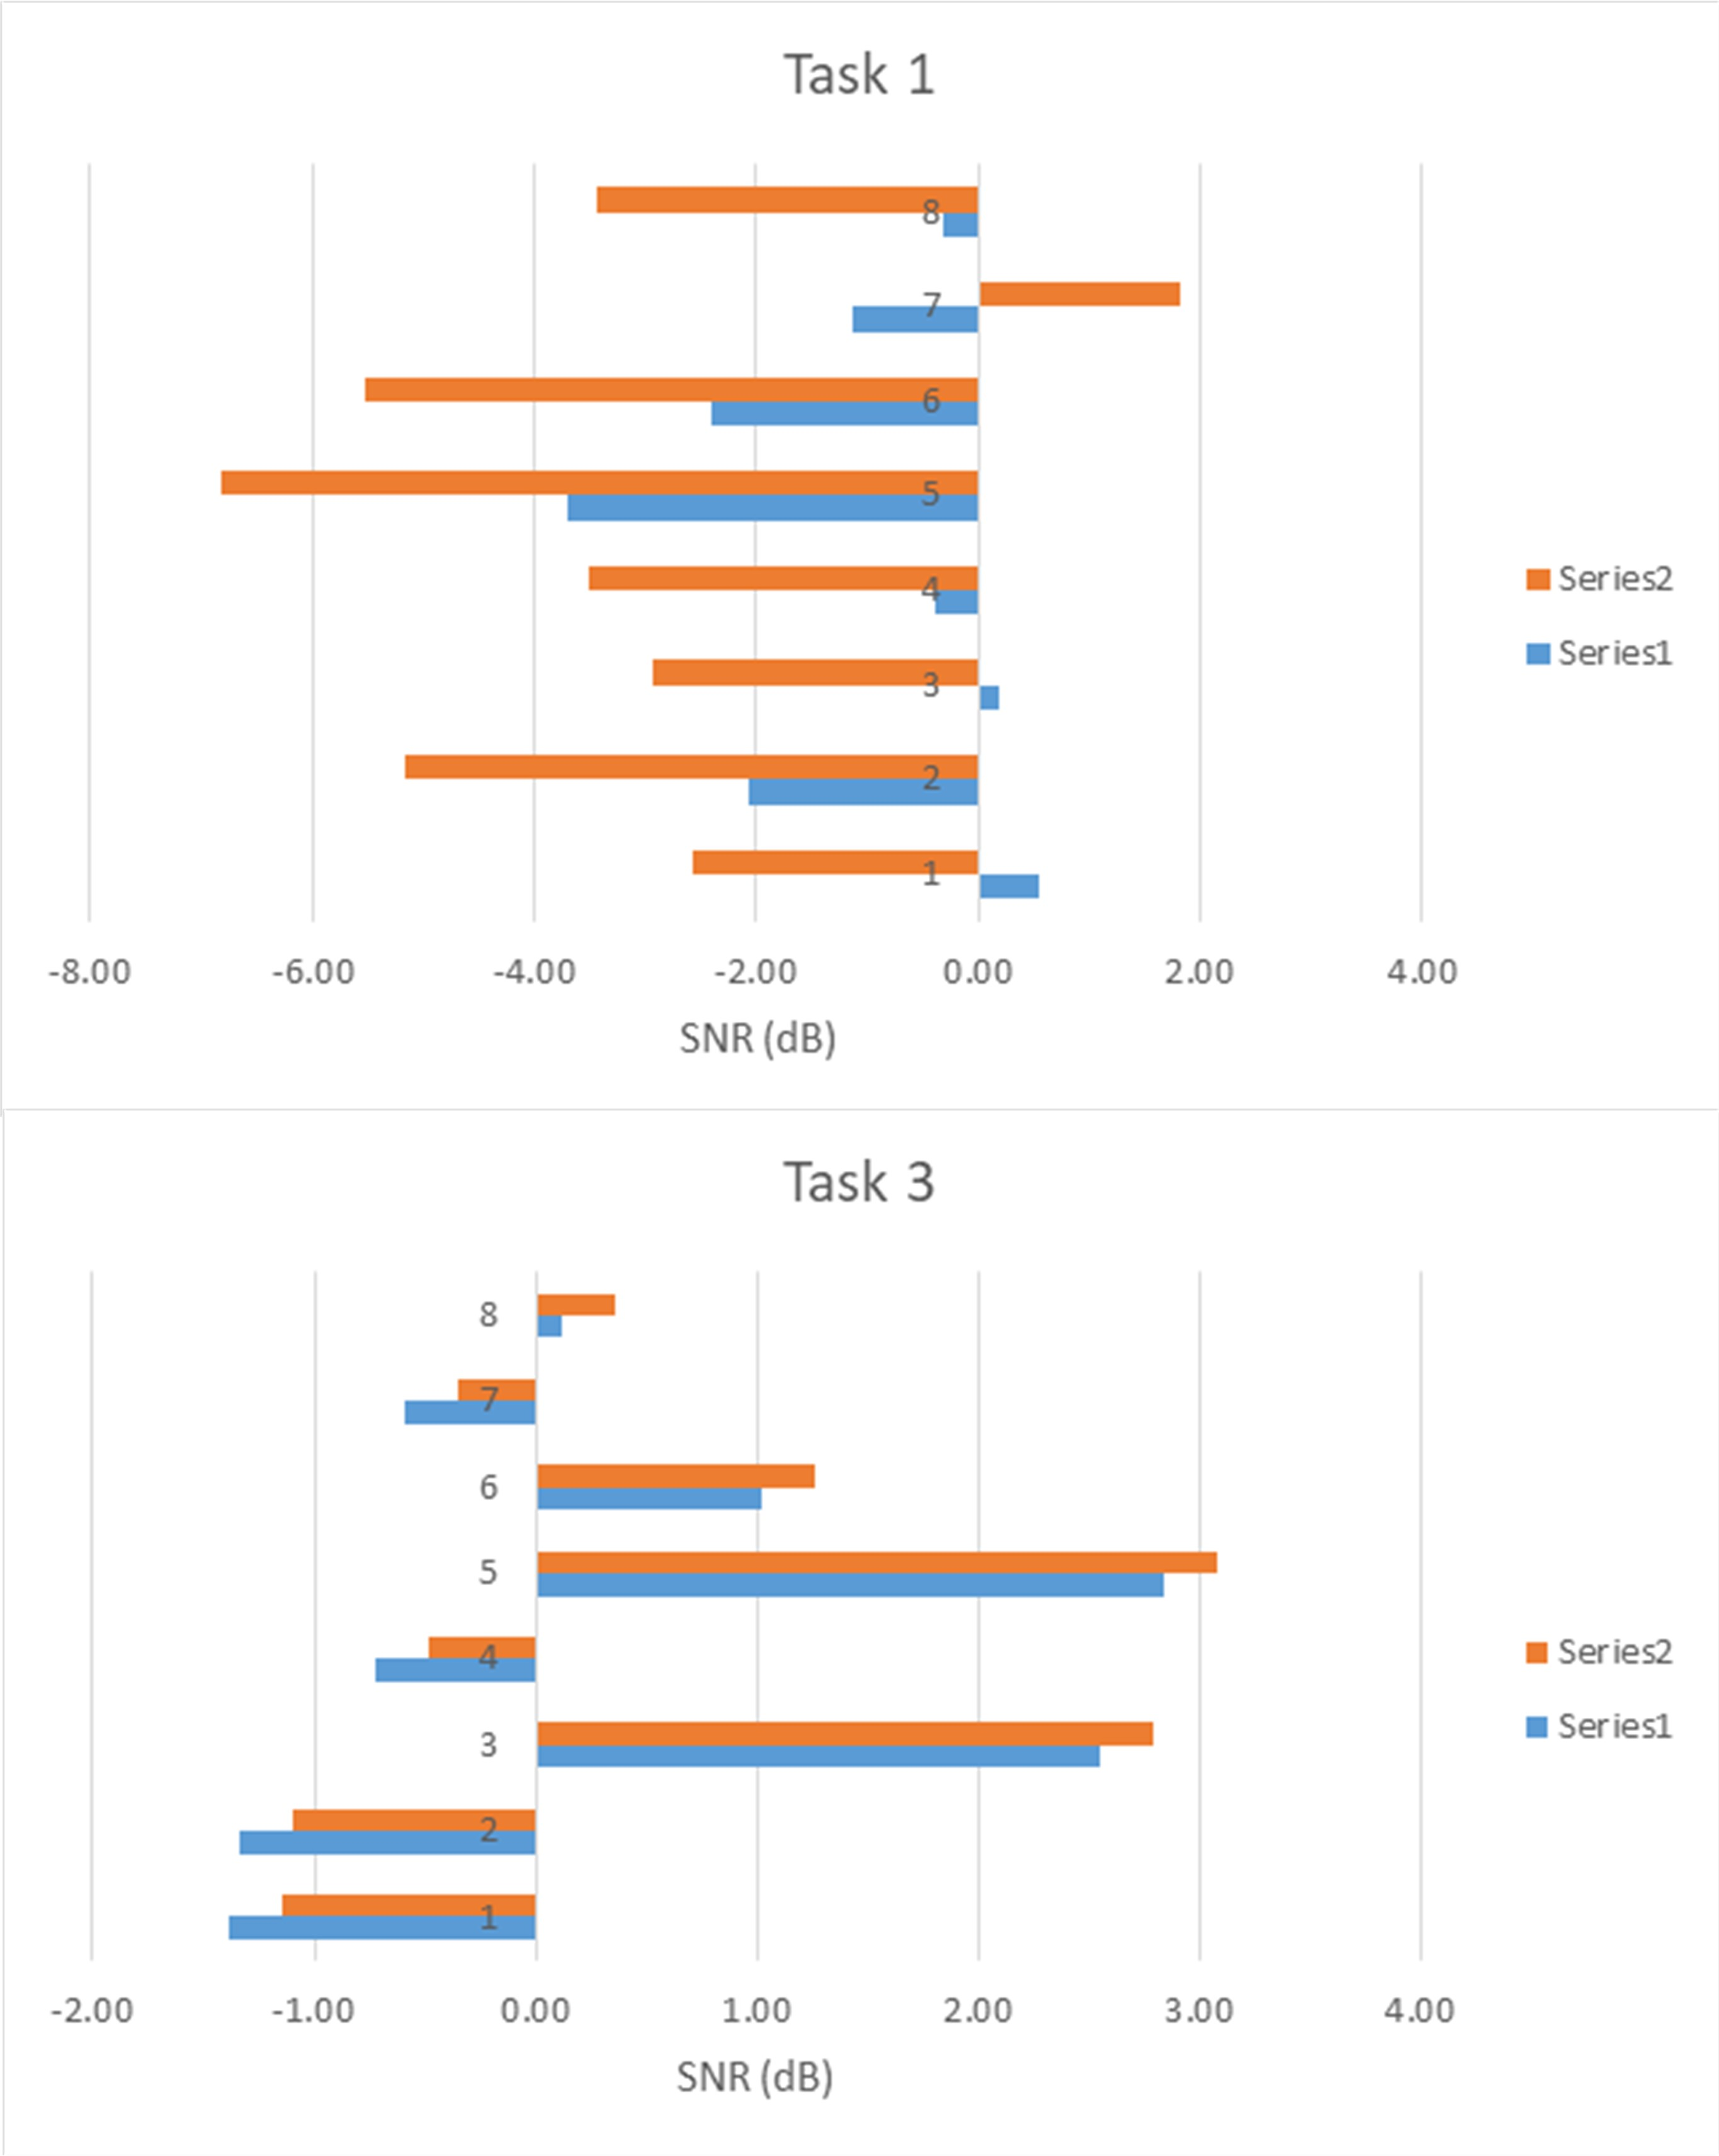
\includegraphics[width=\linewidth]{Figures/SNRchange.jpg} 
	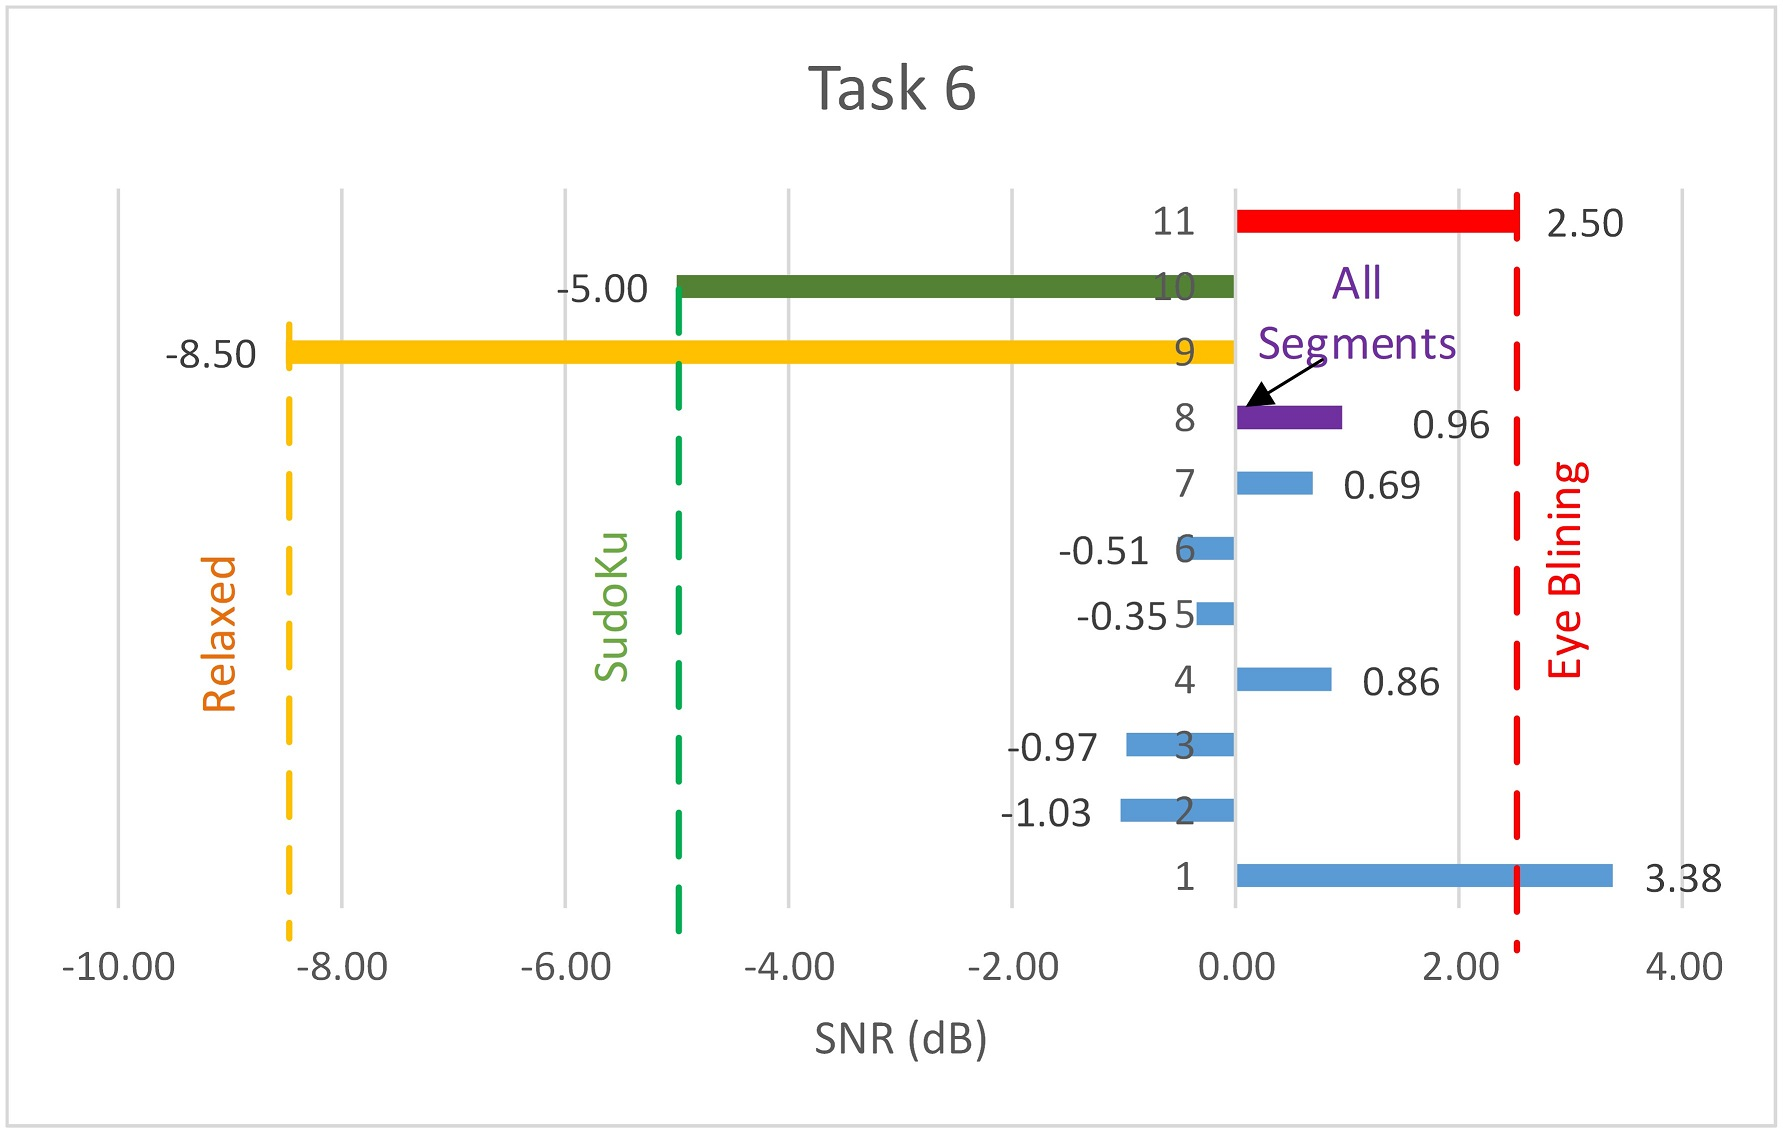
\includegraphics[width=10cm]{Figures/SNRtask6.jpg} 
	\caption{SNR for Task6.} 
	\label{SNR6} 
\end{figure}


\begin{figure}[hbt!]
	\centering
%	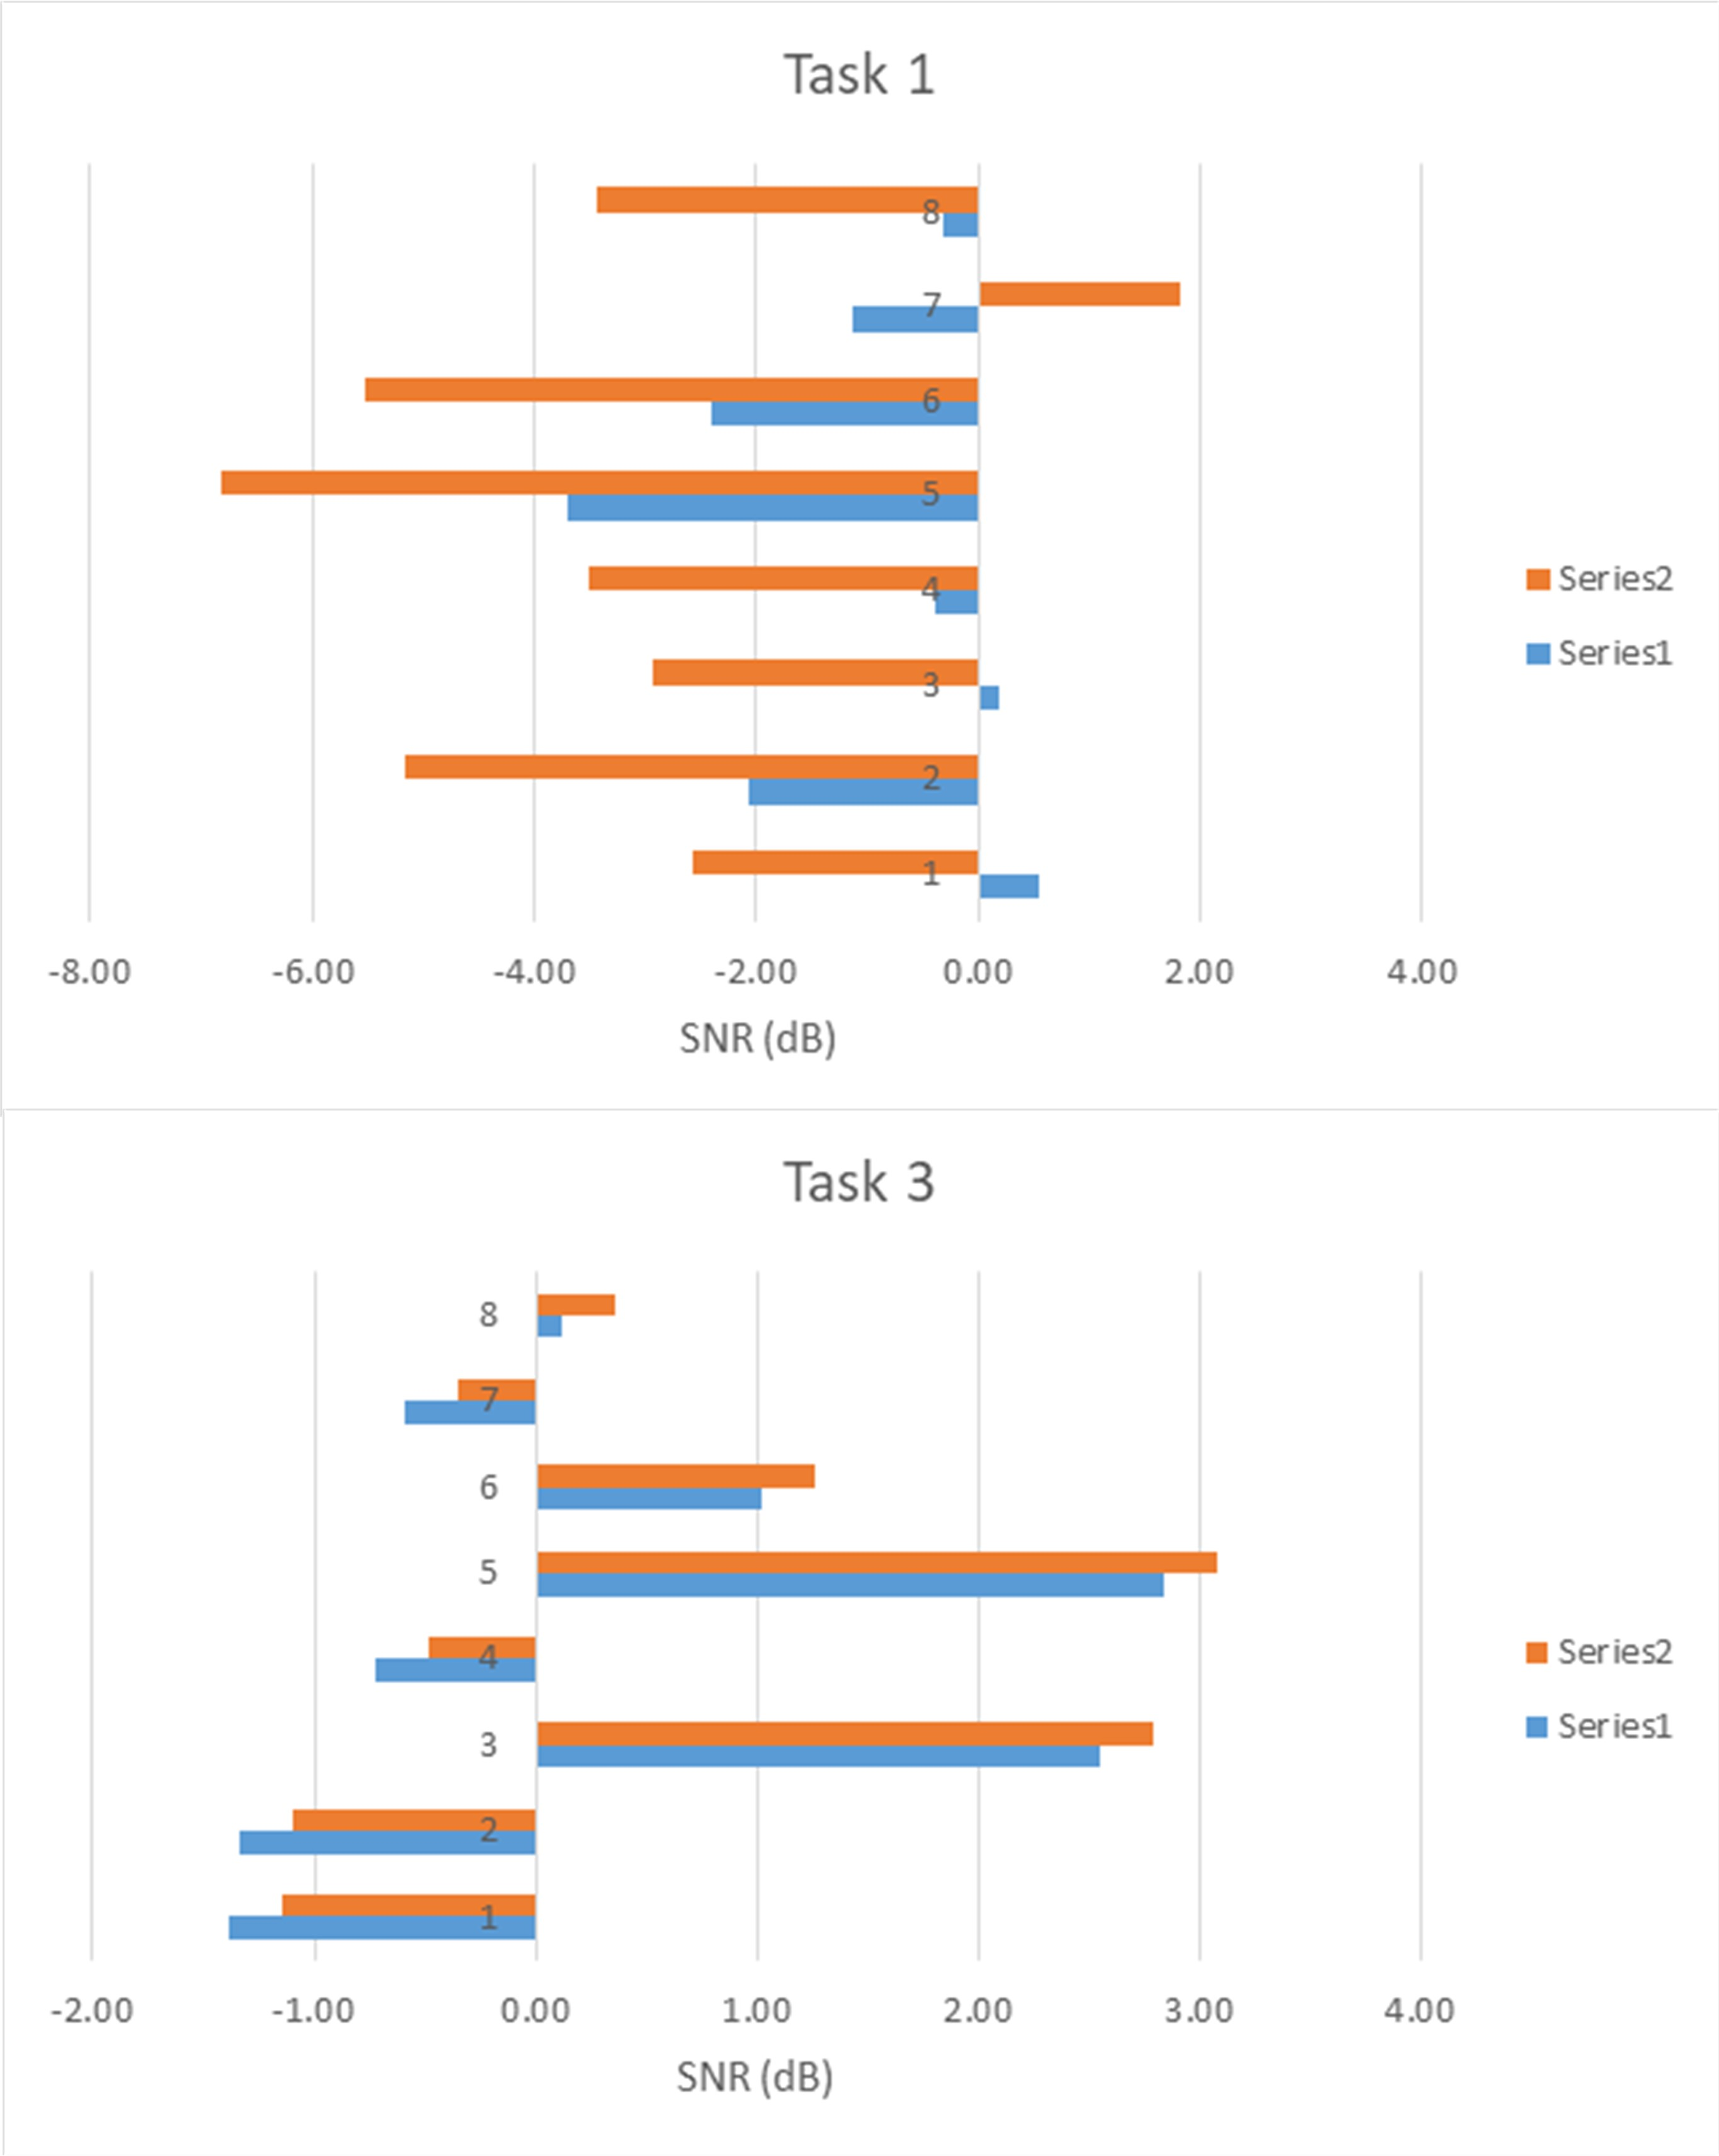
\includegraphics[width=\linewidth]{Figures/SNRchange.jpg} 
	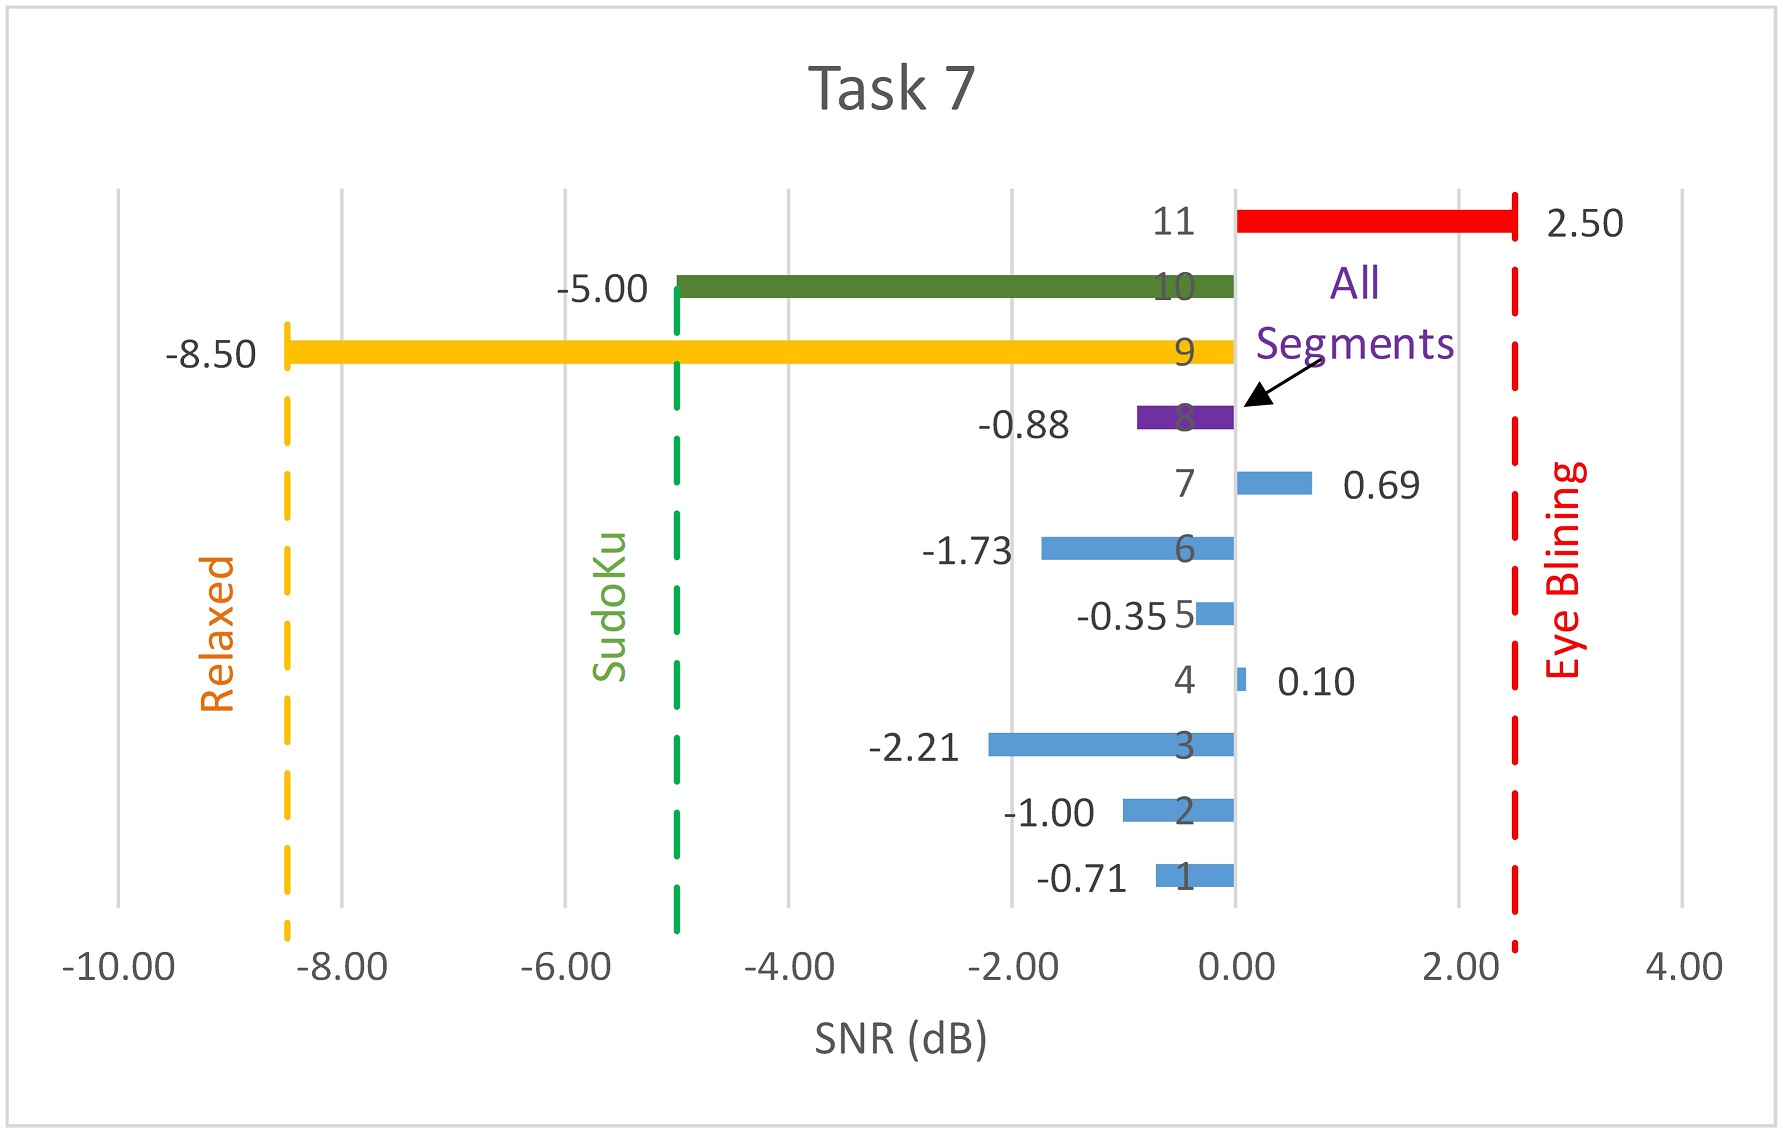
\includegraphics[width=10cm]{Figures/SNRtask7.jpg} 
	\caption{SNR for Task7.} 
	\label{SNR7} 
\end{figure}

From the SNR for all of the experiments it can be seen that the SNR values change between signal segments. For example for the case of Task 7, the SNR is equal to -0.71dB when the EEG recording is examined during the time interval from 4s to 5s (segment 1), while it is +0.69dB during the time interval from 7s to 8s. The worst case for Task7 occurs on the signal segment 3, where the SNR is -2.21dB. Each plot also shows the overall SNR for the Task, which corresponds to the EEG signal from 4s to 8s. The fact that the SNR is not the same between the various signal segments of the task is in accordance with the observation of the alpha band spectrum, where the peak of the 10Hz frequency was varying between signal segments. This variations of the SNR can be justified by the fact that when a person concentrates on performing a specific task, and this effort lasts many seconds, his attention can vary. In other words at some instances his effort is more intensive than in other instances. 

As far as the critical issue on whether the use of EEG signals obtained from a single electrode attached at position Fp1, is concerned, it can be observed that in all tasks and during all segment durations, the SNR achieved is higher than the SNR wall for the ‘relaxed’ and the ‘Sudoku’ case. Unlike the “eye blinking” case, where in almost all cases the SNR achieved is less than the SNR wall.
      
As a general conclusion, based on the EEG recordings available, it can be claimed that the proposed configuration of using EEG from the FP1 position only, can correctly detect the EEG signal and thus determine the intent of the subject. In the case of extreme noise, such as the eye blinking artefacts, once the artefact is detected, the BCI system can ignore the signal segment during the artefact, and thus avoid false detections.  




